% !TeX root = ../main.tex

\chapter{Juggler-ResNet:一种灵活高效的ResNet优化方法}

\section{引言}

近年来,残差网络(如\emph{resnets}、\emph{resnexts})在工业自动化控制和生成中得到了广泛的应用。图.\ref{NIDS}展示了\emph{resnets}在SDIN网络结构中的广泛使用范围。在控制平面上,为了保证SDIN的安全性和隐私性,目前主流的入侵检测系统 (IDS)采用\emph{resnets} \cite{masum2021transfer,song2020real,man2021residual}来检测各种网络恶意攻击,包括拒绝服务(DOS)、用户对根用户(U2R)、远程登录(R2L)等。在基础设施层面上,\emph{resnet}被用于解决许多常见的工业问题,包括故障诊断\cite{8850096}、服务质量(QOS)、自动控制\cite{9166726}、工业浮选过程\cite{9166726,FU2019183}等。与传统的机器学习解决方案 (如决策树、支持向量机)相比,\emph{resnets}在SDIN中的各种AI应用中显示出卓越的性能表现。除了对精度上的要求,推理速度在各种人工智能支持的SDIN和工业应用中也非常重要。以IDS为例,\emph{resnets}的过长的推断时延增加了每次网络监视之间的间隔,导致检测某些关键网络攻击失败。因此,无论是SDIN还是工业自动化生产和管理,在加快卷积神经网络的推理速度的同时并确保准确性具有重大意义,以保证低延迟服务\cite{8850096,9173723,9187678,9173697}。
\begin{figure}[ht]
	\centering
	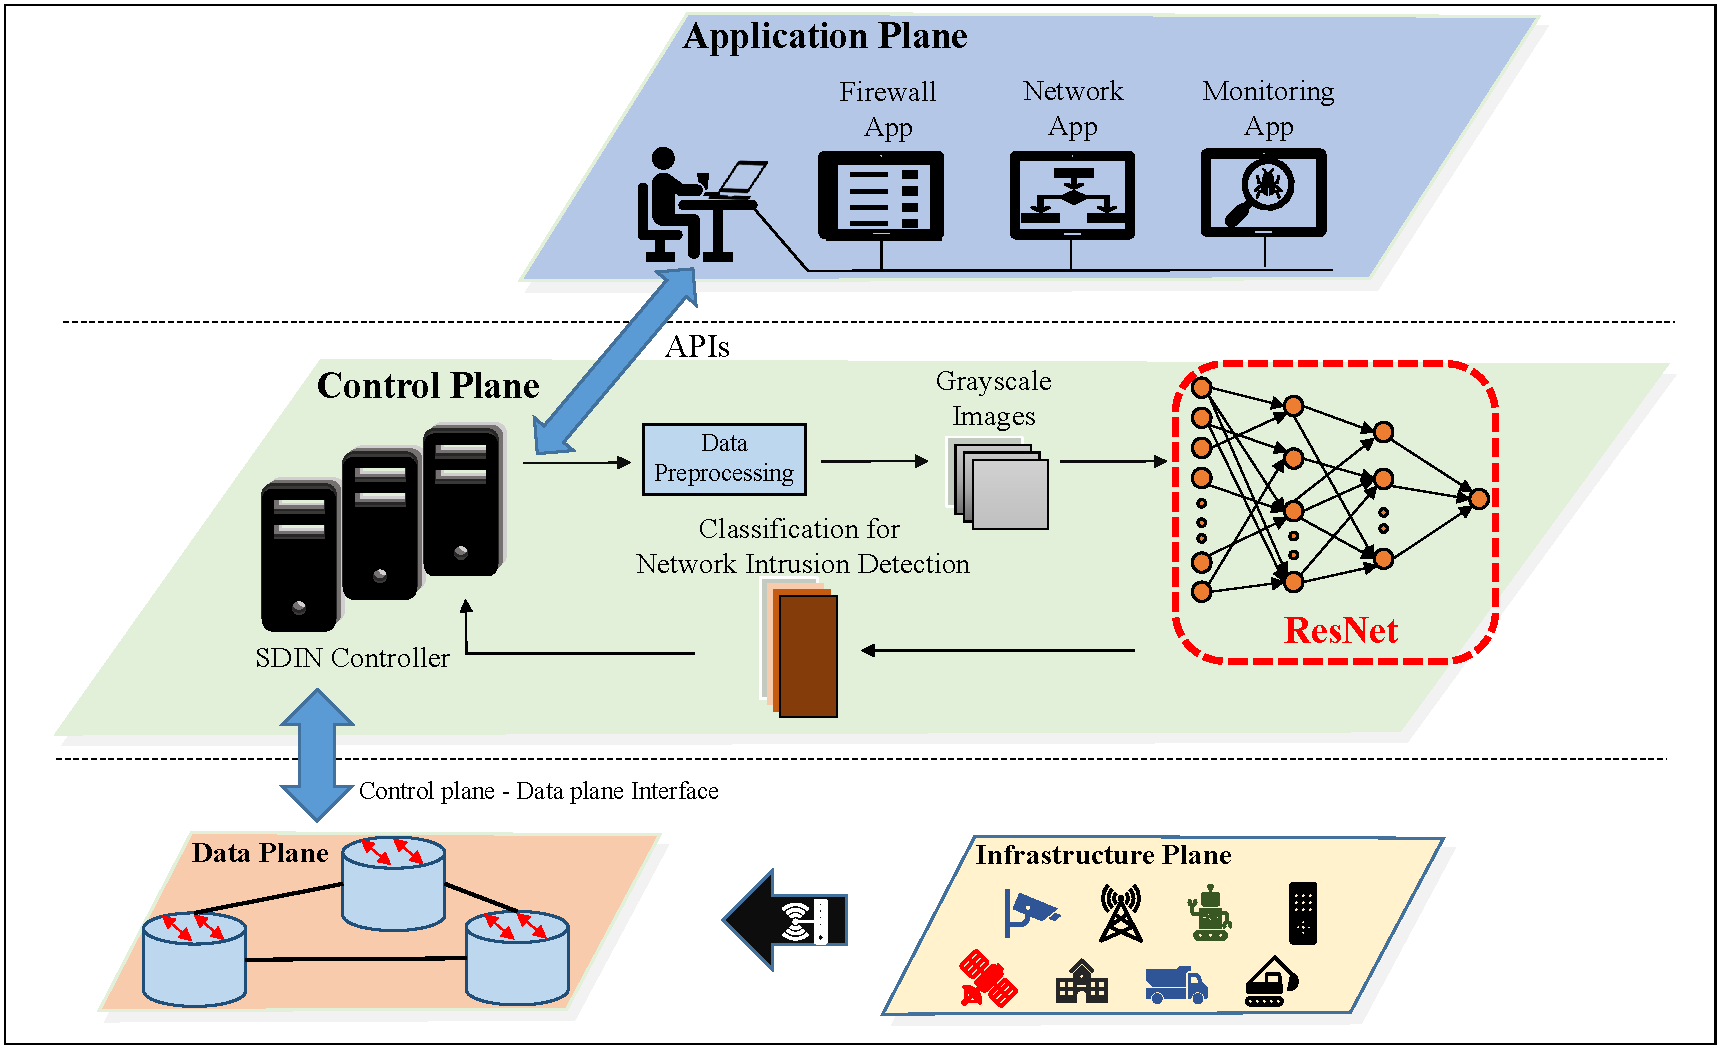
\includegraphics[width=1\textwidth]{figures/Jresnet/FIG1_TII-21-2603.pdf}
	\caption{An illustration of network intrusion detection for the SDIN.}
	\label{NIDS}
\end{figure}

并行化\cite{2020IOS,2018Optimizing,0OPTIMIZING}是提高推理效率的常用方法。以往的研究主要集中在两种最大化神经网络并行化的方法上。1)通过调度CNN算子提高并行性。TensorFlow\cite{2016TensorFlow}、PyTorch\cite{elmohamed}和TVM\cite{2018TVM}等深度学习框架通过对输入图执行贪婪的基于规则的操作来调度操作符并优化输入计算图,该操作在单个CNN操作符内并行化算术运算。Ding\textit{et al.}提出了IOS\cite{2020IOS}通过动态规划算法调度多个操作符以加速网络推理。2)转换计算图以增加CNN算子的粒度。Jia\textit{et al.}\cite{0OPTIMIZING}使用回溯搜索算法将匹配特定模式的多个CNN算子融合到更大的算子中,以提高并行性。TensorRT\cite{tensorRT}不仅融合了算子,而且还在操作系统层面上优化了推理速度,如内核自动调整和动态张量分配等。使用这些方法,可以减少内存访问和内核上下文切换的开销。然而,这些方法仅在计算图上执行优化 (即,在运行时使用解释器解释计算图),它们不会改变网络的总体架构。因此,计算图的优化仍然受到网络结构瓶颈的限制。

\begin{figure*}[!t]
	\centering
	
	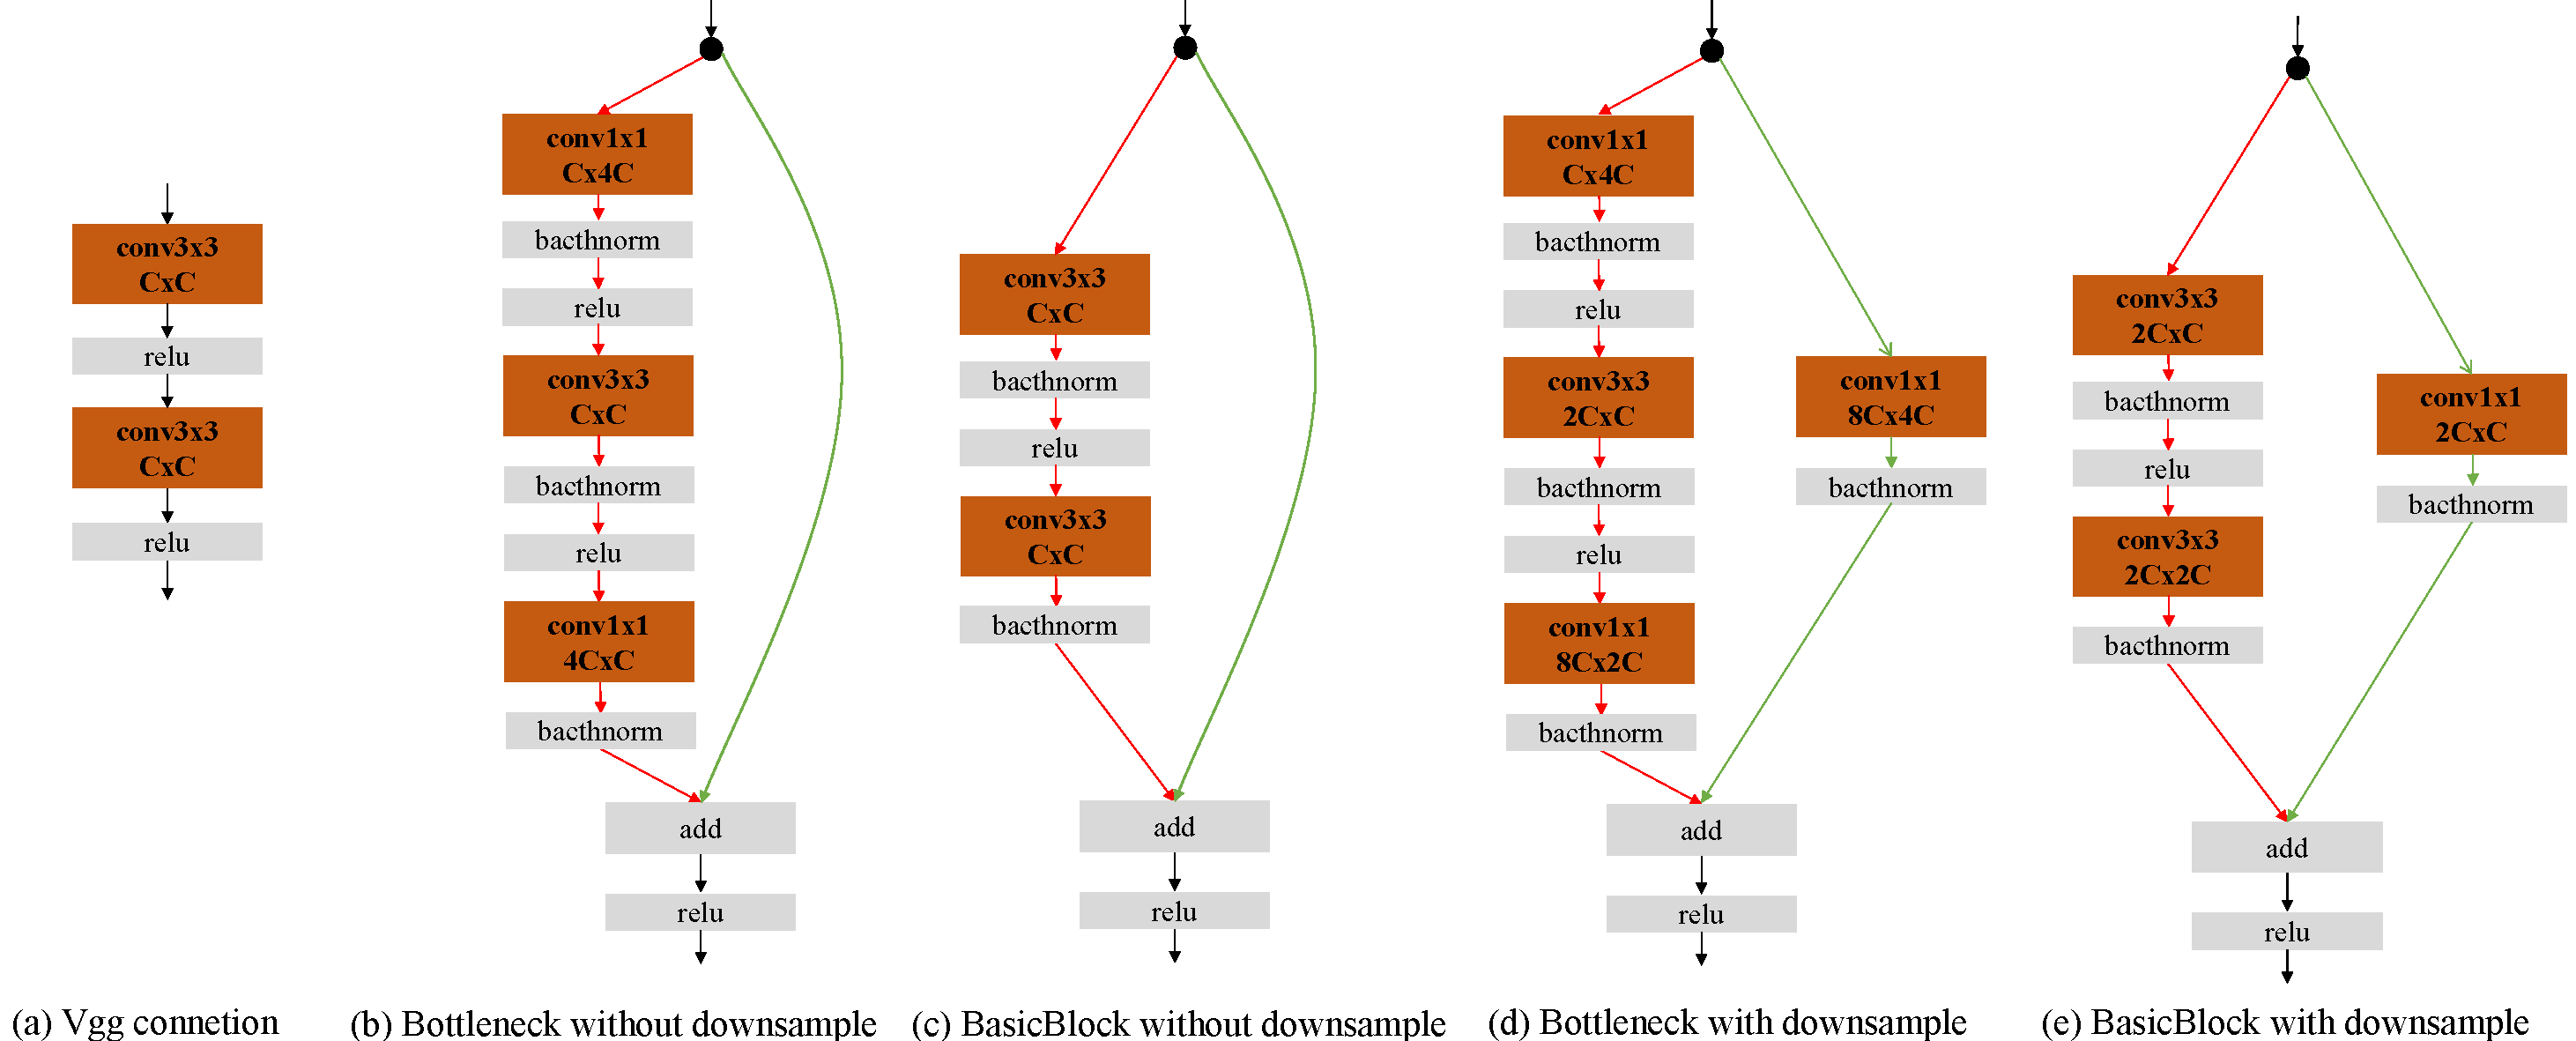
\includegraphics[width=1\textwidth]{figures/Jresnet/FIG2_TII-21-2603.pdf}
	\caption{\emph{vgg}和\emph{resnet}不同的网络连接。图. \ref{dataFlow}. (a) 展示了在vgg网络中最基础的模块。 图. \ref{dataFlow}. (b), (c), (d),和(e) 是在\emph{resnets18-152}中最常用的基础模块, 其中绿色和红色高亮了它们与\emph{vgg}模块不同的数据流。在卷积核上的字母 \emph{\textbf{C}}表示当前卷积核的通道数目。例如, \emph{\textbf{Cx2C}} 表示该卷积核的输入通道数是\emph{\textbf{2C}}, 输出通道数是\emph{\textbf{C}}。}
	\label{dataFlow}
\end{figure*}

多分支体系结构中的两个缺点使得其推理效率较低。1)多分支模型的复杂数据流(例如,\emph{resnet}中的两个分支和\emph{inception}中的分支串联)需要额外的内存空间来存储中间结果,这很容易导致更高的峰值内存使用率、较慢的推理速度和更低的内存利用率。2) 多个细粒度CNN算子的并行度较低。如图.\ref{dataFlow}所示,由于多分支架构具有多个细粒度CNN算子,其数据流比线性拓扑架构更复杂。相比之下,更简单的数据流和粗粒度的操作符使线性拓扑结构在推理中更有效。虽然线性拓扑结构在推理阶段有好处,但其最大的缺点是在训练阶段。线性拓扑结构无法避免训练中的梯度消失问题,这对采用线性拓扑结构的模型获得与多分支结构模型相同的精度提出了挑战。

由于线性拓扑结构有利于推理,而多分支结构有利于训练,因此所提出的变戏法ResNet既具有多分支结构的优点,又具有线性拓扑结构的优点。首先,它在训练阶段保留了具有可融合残差结构的多分支结构的特征提取能力。其次,它可以通过一组融合算子等价地转换为线性拓扑结构,从而在推理阶段充分利用线性拓扑结构的优点。在大范围工作负载下的实验结果表明,Juggler ResNet在SOTA级精度性能下,推理速度提高了2.08-4.4倍。

本章的剩余章节按如下方式组织。第二节介绍背景和动机。第三节介绍所提出的方法。第四节介绍了一些实验和讨论。第五节介绍了相关工作。最后,第六节对本章内容进行总结

\section{相关背景和动机}
本节介绍加速卷积神经网络相关的背景以及卷积神经网络在该领域面临的挑战。


\subsection{卷积神经网络的加速方法}
加快推理速度的一种方法是通过调度CNN算子以增加计算并行性。Tang\textit{et al.}\cite{2018Optimizing}提出了一种贪婪策略,直接在多核CPU上执行所有可用的CNN算子,以充分利用硬件。TensorFlow和PyTorch在单个运算符内并行执行算术运算。
另一种方法是转换卷积神经网络的计算图以优化CNN架构。Jia \textit{et al.} \cite{0OPTIMIZING} 将多个CNN算子合并成一个更大的操作符,以实现更多的并行性。然而,上述研究主要聚焦于对多分支架构的卷积神经网络进行优化。它们不会改变CNN的整体架构,即多分支架构在优化后保持不变。很少有工作关注于将推理阶段的网络结构与训练阶段解耦,以提高推理效率。

\subsection{多分支和单分支卷积神经网络的异同}
\subsubsection{分类精度表现}
ImageNet大规模视觉识别挑战赛 (ILSVRC) 是机器视觉领域最热门、最权威的学术竞赛之一\cite{ILSVRC}。本文从历年比赛中选取出了五个最具有代表性的卷积神经网络模型: \emph{alexnet} \cite{b18}, \emph{vgg} \cite{2014Very}, \emph{google net} \cite{2014Going}, \emph{resnet} \cite{2016Deep} 和 \emph{senet} \cite{2017Squeeze}。如表\ref{fivemodels}所示,存在有明显的趋势表明,更复杂的体系结构网络模型被设计出来用于在比赛中实现较高的图片分类精度性能。与基于线性拓扑结构的模型如\emph{vgg}和\emph{alexnet}相比,\emph{googlenet}采用了精心设计的多分支结构,并且\emph{resnet}提出了一种双分支跳层连接结构,并且\emph{senet}在\emph{resnet}中又引入了通道注意模块。\emph{Google net}, \emph{resnet}, and \emph{senet} 的图片分类准确度性能明显优于线性结构的\emph{alexnet}和 \emph{vgg}。出现这样现象的原因是因为随着网络层数的增加,线性拓扑结构无法避免梯度消失问题。因此,线性拓扑模型很难达到与多分支体系结构相当的图片分类精度性能。
\begin{table}[h]
	\caption{ \emph{alexnet}, \emph{vgg}, \emph{google net}, 和 \emph{resnet}的Top-5图片分类错误率。 Top-5的错误率测试结果是来自于ILSVRC比赛中的数据.}
	\centering
	\label{fivemodels}
	\begin{tabular}{lccccc}
		\hline
		& \textbf{AlexNet} & \textbf{VGG}   & \textbf{Google Net} & \textbf{ResNet}  & \textbf{SENet} \\ \hline
		Year        & 2012    & 2014  & 2014      & 2015    & 2017 \\ \hline
		Layers      & 8       & 19    & 22        & 152     & 152  \\ \hline
		Top-5 error & 15.4\%  & 7.3\% & 6.7\%     & 3.57\%  & 2.25\% \\ \hline
	\end{tabular}
\end{table}

\subsubsection{推理效率表现}
图.\ref{dataFlow} 显示了\emph{vgg}和\emph{resnets}之间基本模块的连接和CNN算子的差异。图.\ref{dataFlow}(a)展示了\emph{vgg}网络线性连接的架构。图. \ref{dataFlow}(b),(c),(d),(e)展示了在\emph{resnet}中使用到的残差结构。右侧的跳层连接 (即,shortcut连接) 减少了梯度返回的损失,避免了梯度消失。同样地,加法运算可以放大输入中的微小干扰,使网络训练收敛更快。


\begin{table}[]
	\caption{
		在 batch size = 32,通道数\emph{\textbf{C}} = 256和 输入图片分辨率resolution = 56的参数设置下,图. \ref{dataFlow}中展示的\emph{vgg}和\emph{resnets}模块在NVIDIA V100的实际推理时间。测试结果是在预热硬件后,取平均20次运行时间所得到的结果。'+'表示该模块是有下采样的。}
	\centering
	\label{infertime}
	\begin{tabular}{ccccc}
		\hline
		& {\textbf{Moudels}} & \begin{tabular}[c]{@{}c@{}}\textbf{Theoretical} \\  \textbf{FLOPs (B)}\end{tabular} & \begin{tabular}[c]{@{}c@{}}\textbf{Time}\\\textbf{usage (ms)}\end{tabular} &\begin{tabular}[c]{@{}c@{}}\textbf{Theoretical}
			\\ \textbf{TFLOPS (B)}\end{tabular} \\ \hline
		&\emph{vgg}          & 118.3            &   7.147         &  \textbf{16.55}                        \\
		&\emph{basicblock}   & 118.4            &  8.312          &  14.24                  \\ 
		&\emph{basicblock+}  & 92.16            &   9.793         &   9.41                 \\ 
		&\emph{bottleneck}   & 112.4            &   16.845        &   6.67                   \\ 
		&\emph{bottleneck+}  & 135.04           &   25.714        &   5.25                \\ \hline
		
	\end{tabular}
\end{table}

为了详细分析多分支和单分支网络在推理效率上的差异,本文在NVIDIA V100上进行了实验,以计算它们的运行时间。表\ref{infertime}显示了在NVIDIA V100 GPU上使用compute unified device architecture (CUDA)10.2测试的理论浮点运算次数(FLOPs)和实际运行的时间。如表\ref{infertime}所示 the theoretical FLOPs of \emph{vgg}, \emph{basicblock}, \emph{basicblock+}, \emph{bottleneck}, 和\emph{bottleneck+}的理论双精度浮点计算此处几乎是处于同一个水平。然而,线性拓扑结构的\emph{vgg}却有最高的理论每秒tera浮点运算(TFLOPS),这归因于线性拓扑结构网络没有额外的内存开销。此外,在相同的理论双精度浮点数操做次数下,它优于其他多分支体系结构模型,比其他四种模型快了17.6\%—165.3\%。因此,理论双精度浮点总操做次数和实际每秒双精计算次数之间的这种明显的差异可归因于两个重要因素:内存访问开销和并行度。在多分支模型中,内存访问开销占用了很大一部分时间,因为两个分支的\emph{resnets}需要存储两个独立特征副本来执行独立的计算过程(即 在图\ref{dataFlow}中用红色和绿色高亮的两个计算流)。相反,线性拓扑结构 (图.\ref{dataFlow}(a))将其唯一的前一层的输出作为输入,并将输出输出到其唯一的后一层,这样简单的计算流使得在整个计算过程中不需要任何额外的内存开销。值得注意的是,表\ref{infertime}表示出\emph{vgg}和\emph{basicblock}具有相同数量的双精度浮点操做次数。但是\emph{vgg}的实际每秒双精度计算次数高于\emph{basicblock},这表明该性能的提升是完全来得益于它的线性拓扑结构。另一方面,使用粗粒度CNN算子的模型可能比使用细粒度CNN算子的模型更快。以前的研究表明,粗粒度CNN算子更有利于硬件并行性。表\ref{infertime}显示\emph{vgg}和\emph{basicblock}具有最高的每秒双精度计算次数。它们都只有3x3卷积核,而其他模型有多个1x1卷积核。

\subsection{卷积核执行效率表现}
表\ref{channel}的第五列说明了卷积内核大小和通道数对双精度浮点数每秒操作数(TFLOPS)的影响。在所有不同通道数和大小的卷积核中,3x3卷积核的双精度浮点数每秒操作数最高,为6.60-6.87。1x1卷积核的执行效率最低,只有4.79-6.05。5x5卷积核和7x7卷积核TFLOP几乎处于同一水平,分别为6.06-6.41和6.30-6.41。值得注意的是,1x1卷积核太小,无法充分利用硬件并行能力,这导致它与其他大卷积内核(3x3,5x5,7x7)之间的TFLOPS存在着显著的差距。它比执行效率最高的3x3卷积核慢43\%。然而,3x3卷积核、5x5卷积核和7x7卷积核之间只有很小的区别。因此,我们可以得出结论,大尺寸卷积核可以充分利用硬件并行能力。

笔者认为,3x3卷积核在执行效率上的优势与3x3卷积核的优化和填充有关。对于优化,Winograd\cite{LavinG16}是一种用于加速3x3卷积核的经典算法,该算法已经在cuDNN(NVIDIA CUDA深度神经网络库)中得到充分的实现。例如标准F(2x2,3x3)Winograd,3x3卷积核的浮点乘法操做数量是原始乘法数量的4/9。另一方面,为了确保特征图的尺寸在经过卷积核运算后不会发生改变,一种常用的做法是在特征的图周围填充0。而较大的特征图需要更多的0来填充。因此,conv5x5和conv7x7执行的无用计算比conv3x3多。

表\ref{channel}的第三列还说明了通道数对双精度浮点操做总次数的影响。双精度浮点操做总次数随着通道数的增加而增加。双精度浮点操做总次数的实际增长模式符合Eq.\ref{parameters}。值得注意的是,通道数目为2048的7x7卷积核的双精度浮点操做总次数超过了NIVIDIA V100理论计算能力上限,因此与通道数目为1024的conv7x7相比,执行效率反倒还降低了1.69\%。综上所述,当双精度浮点操做总次数小于硬件计算能力的峰值时,卷积核的执行效率总是随着双精度浮点操做总次数的增加而增加的。

\begin{equation}
\begin{aligned}
\label{parameters}
Parameters &= \sum_{i=0}^n Inc_i \times Outc_i \times KernelSize_i^{2}
\end{aligned}
\end{equation}
$i$表示一个卷积核, $n$表示一个结构中卷积核的总数目。$Inc_i$和$Outc_i$是卷积核$i$的输入输出通道数,$KernelSize$是卷积核$i$的尺寸大小。

\begin{table}[h]
	\caption{
		卷积核在不同尺寸大小和不同通道数目下设置下,输入图像分辨率为56x56,禁用cuDNN优化在NVIDIA V100上的推理时间。结果是硬件预热后20次推理时间的平均值。}
	\label{channel}
	\centering
	\begin{tabular}{cccccc}
		\hline
		\textbf{Kernel Size} & \textbf{Channel} & \textbf{FLOPs(B)} & \textbf{Time(ms)} & \textbf{TFLOPS(B)} \\
		\hline
		\multirow{3}{*}{1x1}
		&512	&26.35 &5.50	&4.79	\\
		&1024	&105.28	&18.47	&5.70	\\
		&2048	&421.12	&69.55	&6.05	\\
		
		\hline
		\multirow{3}{*}{3x3}
		&512	&236.82	&36.46	&6.49	\\
		&1024	&947.24	&141.66	&6.69	\\
		&2048	&3788.48	&550.25	&6.88	\\
		
		\hline
		\multirow{3}{*}{5x5}
		&512	&657.62	&108.51	&6.06	\\
		&1024	&2630.72	&412.73	&6.37	\\
		&2048	&10522.88 &1639.18	&6.42	\\
		
		\hline
		\multirow{3}{*}{7x7}
		&512	&1288.96	&204.51	&6.30	\\
		&1024	&5156.16	&804.13	&6.41	\\
		&2048	&20624.64 &3271.01	&6.30	\\
		
		\hline
	\end{tabular}
\end{table}

\subsection{卷积核参数膨胀}
\label{para_expan}
重参数化\cite{2019ACNet,2021Diverse}允许将训练中获取的参数注入新的网络架构,从而利用网络架构优点,转变卷积网络计算模式。最近,Ding\textit{et al.}提出了ACNet\cite{2019ACNet},它使用非对称的1x3卷积核和3x1卷积核来提高3x3卷积核在训练中的性能,并将它们合并到部署中的3x3卷积核中以实现性能的提升。Diverse Branch Block \cite{2021Diverse}提出了一种通用的Inception块结构来代替Inception网络中原始的卷积核。然而,这种技术严重依赖于网络模型的原始体系结构。在没有适当设计的情况下直接将该技术应用于网络体系结构可能会导致卷积核参数膨胀的问题,致使其计算成本开销可能超过转换网络体系结构所带来的收益。

\begin{figure}[ht]
	\centering
	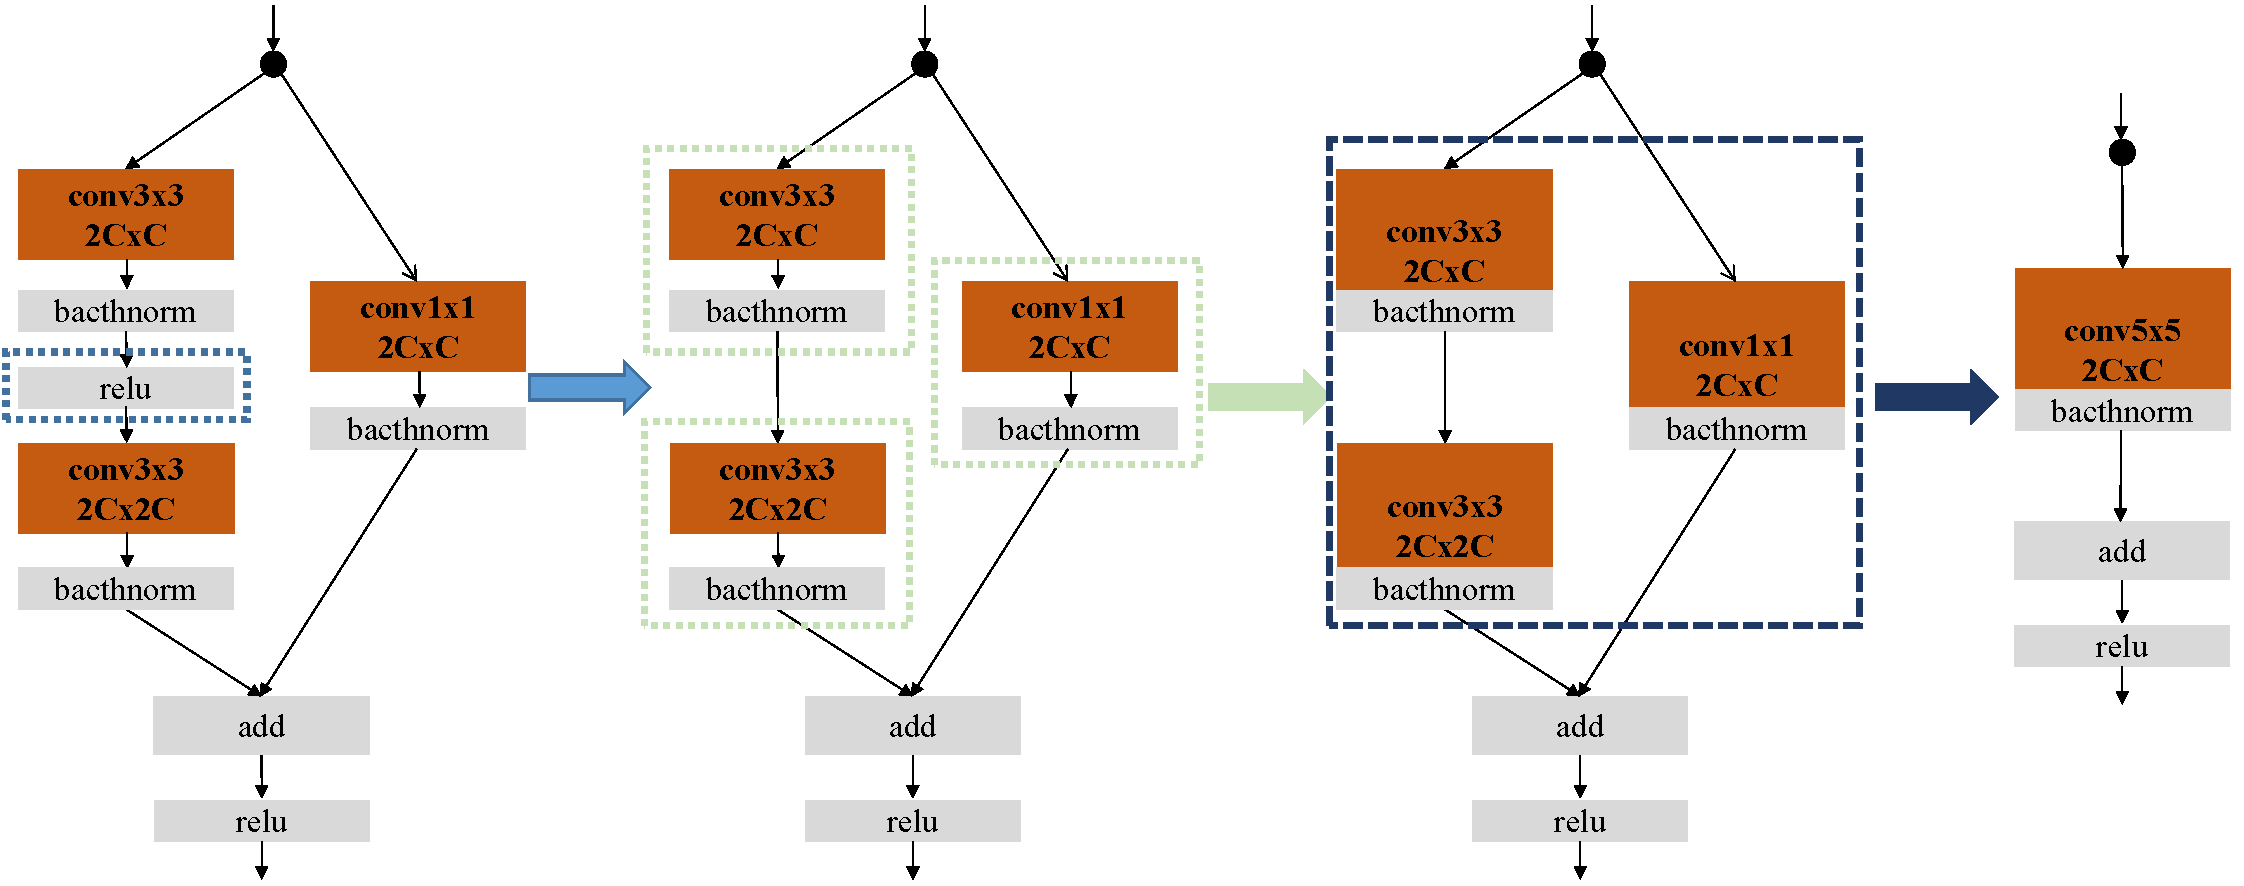
\includegraphics[width=1\textwidth]{figures/Jresnet/FIG3_TII-21-2603.pdf}
	\caption{An illustration of converting \emph{Basicblock} into liner-topology architecture.}
	\label{basic_block_merge}
\end{figure}
例如,将\emph{basicblock}和\emph{bottleneck}等效地转换为线性拓扑结构会导致参数膨胀的问题。具体地来说,图.\ref{basic_block_merge}展示了将\emph{basicblock}转换为线性拓扑结构的过程。首先,它需要删除两个卷积层之间的relu层。接下来,将batchnorm层融合到卷积层中以合并两个卷积层。最后,两个3x3卷积核可以等效地转换为一个5x5卷积核\cite{2016Rethinking}。但是,5x5卷积核的双精度浮点操做总次数明显大于两个3x3卷积核的总操作次数之和。Eq.\ref{parameters}展示了合并后的5x5卷积核的参数比两个3x3卷积核的总参数之和还多1.4倍。 同样地,\emph{bottleneck}也存在同样的问题。Eq.\ref{parameters}显示将\emph{bottleneck}结构转换为线性拓扑结构后,参数扩展了2.76倍。在这种情况下,影响推理效率的最主要因素是双精度浮点操做总次数。我们在NVIDIA V100上的结果表明,参数膨胀的问题会将推理延迟增加12.5-20.7\%。总的来说,直接转换\emph{bottleneck}和\emph{basicblock}结构为线性拓扑结构会显著增加参数量,覆盖了转换为线性拓扑结构的所带来简化计算流的收益。

\subsection{结论}
实验表明,在推理阶段,线性拓扑比多分支结构更有效。这表明更简单的数据流和更粗粒度的运算符有利于推理。此外,线性拓扑结构不需要存储中间结果,因此减少了内存访问和内核上下文切换开销。

\section{Juggler-ResNet优化方法}

\subsection{概述}
基于以上结果,我们的分析表明1)线性拓扑结构比多分支结构更有效。在双精度浮点操做次数相同的情况下,大而CNN算子比小而碎的CNN算子计算效率更高;2) 线性拓扑结构很难实现与多分支结构相同的精确性能。\emph{resnet}中的快捷连接减少了梯度返回的损失,避免了梯度的消失;3) 将resnet中的残差结构直接转换为线性拓扑结构会导致参数膨胀的问题,这会覆盖转换为线性拓扑所带来简化计算流的收益。


\subsection{Juggler ResNet}


\begin{figure}[h]
	\centering
	\subfigure[Fusible residual structure
	]{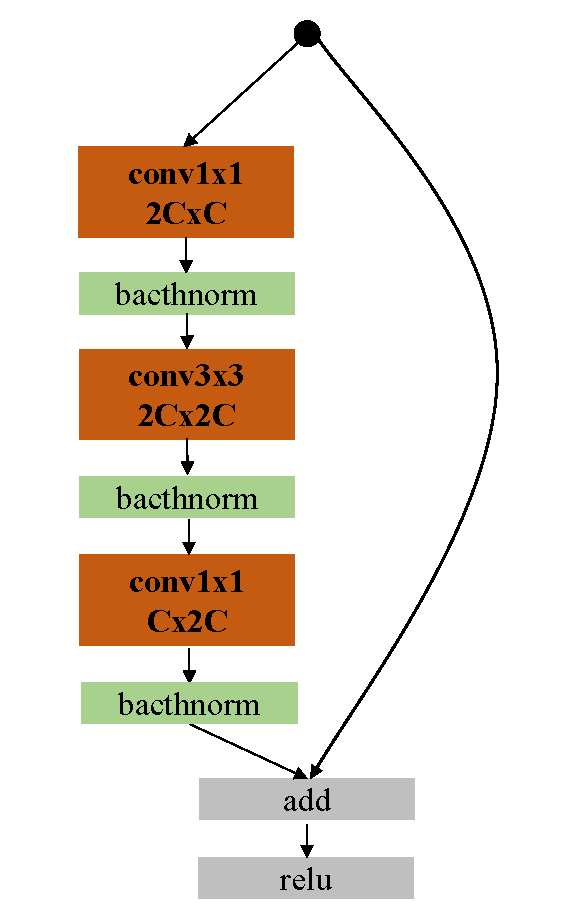
\includegraphics[width=0.45\textwidth]{figures/Jresnet/FIG4(a)_TII-21-2603.pdf}
		\label{fuse_1}}
	\subfigure[Fusible residual structure with downsample]{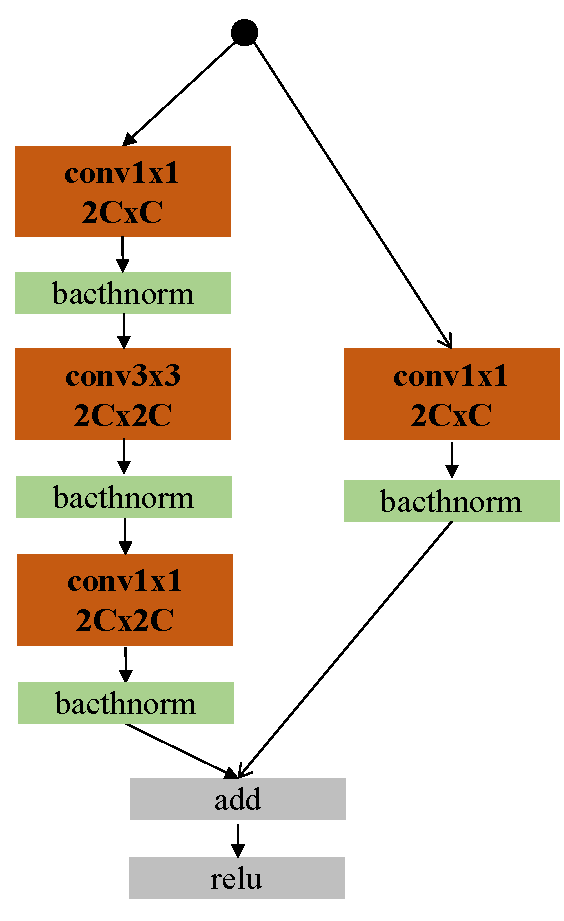
\includegraphics[width=0.45\textwidth]{figures/Jresnet/FIG4(b)_TII-21-2603.pdf}
		\label{fuse_2}}
	\caption{The design of fusible residual structure in Juggler-Resnet.}
	\label{our_fusible_multibranch}
\end{figure}

为了克服上述所提到的各个挑战,我们提出了一种全新的残差结构,名为Juggler ResNet,如图所示\ref{our_fusible_multibranch}。它由8层网络和4种不同的运算符组成,包括\emph{convolution}、\emph{batchnorm}、\emph{relu}和\emph{add}层。值得注意的是,我们的结构同样也采用了两个分支的跳层连接,用以减少卷积神经网络在训练时梯度消失的问题。“双分支”的跳层连接在两个互不相邻的图层之间添加具有权重的交叉链接。其中,带有下采样的残差结构在跳层连接上还有一个\emph{convolution}和\emph{batchnorm}层。\emph{add}操作可以放大输入中的轻微干扰,使网络训练收敛更快。同时,还移除\emph{convolution}和\emph{convolution}层之间的\emph{relu}层以保证两个\emph{convolution}层的等价融合,但保留最后一个\emph{relu}层以确保结构级别的非线性关系。Juggler ResNet和原始\emph{ResNet}之间的主要区别在于\emph{convolution}层的设计。


如第节\ref{para_expan}所讨论到的,原始\emph{resnet}模型中的参数膨胀问题阻止了残差结构的等价合并:1)在\emph{basicblock}中的3x3卷积核参数将膨胀增加至原来的1.39倍;2)在\emph{bottleneck}(图. \ref{dataFlow} (b),(d))的通道膨胀问题将使得参数增加2.76倍。基于这一观察,我们采用两个1x1卷积核和一个3x3卷积核替换这些结构。因为两个1x1卷积核和一个3x3卷积核可以等效地融合为一个3x3卷积核,而参数量保持不变。对于通道扩展问题,我们将1x1卷积核的输入通道数修改为C,将输出通道数修改为2C。与\emph{bottleneck}中的通道数相比,我们选择在3x3卷积核处扩大通道数而不是减少通道数的原因如下:1)它仅用于训练阶段,在推理阶段只部署等价的线性结构以加速推理。因此,计算量的增加并不会影响推理阶段。2) 在3x3卷积核处加宽通道数目可减少因移除relu层而导致的图片分类精度降低的问题。总之,增加3x3卷积核的通道数确实会增加训练期间的计算量,但它也可以在训练阶段提取更多的特征信息。可融合的残差结构的等效线性结构的参数大小约为\emph{bottleneck}和\emph{basicblock}的1.12倍。


\subsection{等价转换策略}
基于Juggler-ResNet,我们提出了三种可以等价将残差结构转换为线性结构的算子:1)卷积层和批量归一化融合算子2)卷积层垂直融合算子3)卷积层水平融合算子
。
\subsubsection{卷积核和批归一化融合算子}
\label{sub1}
为了为后续合并两个直接相连接的卷积核,我们首先需要将batchnorm层融合到卷积内核层中。幸运的是,可以将batchnorm层融合到卷积内核层中,而无需任何额外开销和损失。将卷积内核层的输出作为输入输入到batchnorm层,如下公式所示:
\begin{equation}
\begin{aligned}
\label{BN_eq}
BN(Conv(X)) &= \gamma * \frac{WX + b - mean}{\sqrt{var}} + \beta \\
&= \frac{\gamma * WX}{\sqrt{var}} + \frac{\gamma * (b - mean)}{\sqrt{var}} + \beta
\end{aligned}
\end{equation}
$X$是输入参数矩阵。$W$和$b$分别是权重矩阵和偏置矩阵。$mean$和$var$分别是输入参数矩阵的$X$平均值和方差,$\gamma$和$\beta$分别表示在正则化层中的比例因子和偏置注意到Eq.\ref{BN_eq}其实是卷积核层的表达方式,于是我们令:
\begin{equation}
\begin{aligned}
&W_{fused} = \frac{\gamma * W}{\sqrt{var}} &B_{fused} = \frac{\gamma * (b - mean)}{\sqrt{var}} + \beta \\
\end{aligned}
\end{equation}
其中$W_{fused}$和$B_{fused}$ 分别是融合后的参数矩阵和偏置矩阵, $Conv_{fused}$是将批归一化层融合到卷积核层之后的表达式。然后,我们就有了下列批归一化层和卷积核层的等价表示:
\begin{equation}
\begin{aligned}
Conv_{fused}(X) &= BN(Conv(X)) \\
&= W_{fused}X + B_{fused}
\end{aligned}
\end{equation}
因此,构造一个卷积核层等价于一个卷积核后跟一个batchnorm层是可行的。



\subsubsection{卷积核层垂直合并算子}
\label{sub2}
将batchnorm层融合到卷积核层后,图.\ref{our_fusible_multibranch}(a,b)中的每个卷积核层就会直接连接,这意味着每个卷积核层将其前一个卷积核层的输出作为输入,并将输出馈送到其唯一的下一个卷积核层。因此,有如下公式成立:
\begin{equation}
\begin{aligned}
Conv_2(Conv_1(X)) &= W_2(W_1X+b_1) + b_2 \\
&= W_2W_1X + W_2b_1 + b_2 \\
&= (W_2W_1)X + (W_2b_1 + b_2)
\end{aligned}
\label{eq4}
\end{equation} 
注意到 Eq(\ref{eq4})实际上是卷积核层的表示,于是我们令:
\begin{equation}
\begin{aligned}
&W_{fused} = (W_2W_1) &b_{fused} = (W_2b_1 + b_2)
\end{aligned}
\end{equation}
然后,我们有以下两个直接项链卷积核层的等价表示:
\begin{equation}
\begin{aligned}
Conv_{fused} &= W_{fused}X + b_{fused}
\end{aligned}
\end{equation} 

\begin{figure}[h]
	\centering
	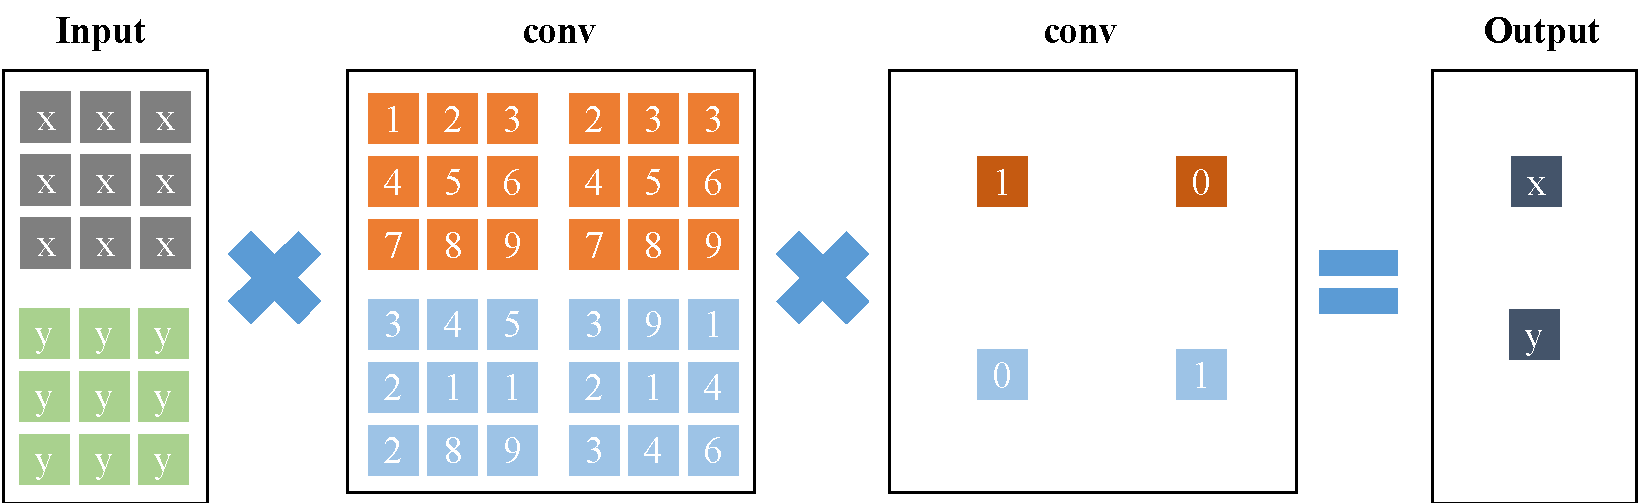
\includegraphics[width=1\textwidth]{figures/Jresnet/FIG5_TII-21-2603.pdf}
	\caption{Illustrations of fusing conv3x3 and conv1x1.}
	\label{fuse_131}
\end{figure}
为了进一步解释,将特征映射[1,2,3,3]作为输入,并将其输入到直接相连的1x1卷积核和3x3卷积核层,输出为[1,2,1,1]。实际计算过程如图所示。这可以看作是将3x3卷积核的参数作为输入并输入到1x1卷积核,并使用输出作为参数对输入进行卷积操做。

\subsubsection{卷积核水平融合算子}
\label{sub3}
卷积层水平融合算子可以将在图\ref{our_fusible_multibranch}(b)中所示跳层连接上1x1卷积核融合,从而消除多分支结构。要进行水平合并,首先需要将1x1卷积核扩展到3x3卷积核以使它们之间的尺寸大小相匹配。1x1卷积核可以看作是3x3卷积核的一个特例,这意味着它可以用3x3卷积核表示。如图\ref{conv1_expand}所示,1x1卷积核可以通过在卷积核周围填充零来扩展到3x3卷积核。然后,通过将3x3卷积核添加到扩展后的3x3卷积核的中心点,便可以将两个卷积核3x3水平合并为一个3x3卷积核。

\begin{figure}[h]
	\centering
	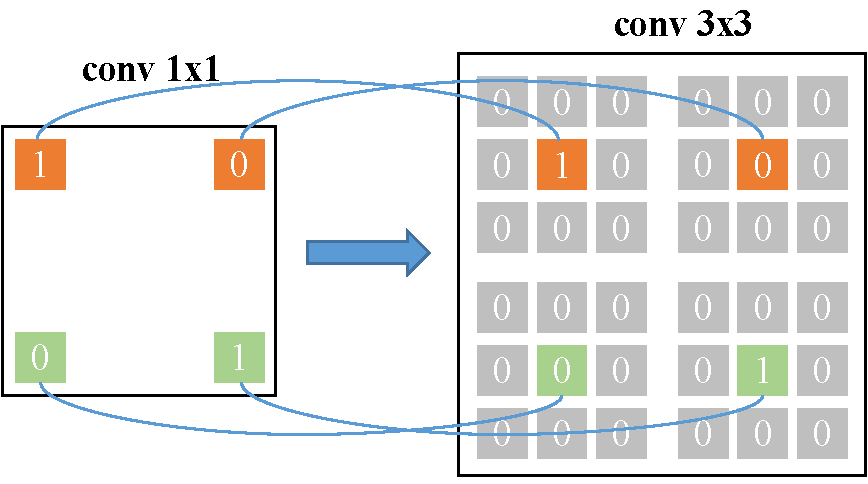
\includegraphics[width=1\textwidth]{figures/Jresnet/FIG6_TII-21-2603.pdf}
	\caption{Equivalent conv3x3 representation of conv1x1 convolution kernel.}
	\label{conv1_expand}
\end{figure}


\begin{algorithm}[H]
	\caption{Convert Juggler-ResNet into liner-topology architecture}
	\SetKwFunction{Unio}{Union}
	\SetKwInOut{Input}{input}
	\SetKwInOut{Output}{output}
	
	\Input{A multi-branch architecture Juggler-ResNet $G_0$, a list of fusible residual structure $\{g_{1},g_{2},g_{3}......g_{n}\}$ of Juggler-ResNet and each $ g_{i}$ has convolution kernels layers $L =$ $\{conv_{1},conv_{2},conv_{3},sconv_{4}\}$, three fusion operator $F_{batch}(.)$ in \ref{sub1}, $F_{conv}(.)$ in \ref{sub2} and $F_{expand}(.)$ in \ref{sub3}.}
	\Output{Liner-topology architecture Juggler-ResNet $G_1$.}
	\BlankLine
	// $sconv_{4}$ represent the convolution kernel on the shortcut\; 
	// connection in a fusible residual structure $ g_{i}$ with downsampling\;
	\For{$i=1,\cdots,n$}{
				$g_i = F_{batch}(g_i)$\;
				$Conv_{m} = F_{conv}(g_i.conv_{1},g_i.conv_{2})$\;
				$Conv_{m} = F_{conv}(Conv_{m},g_i.conv_{3})$\;
				\If{$g_i.sconv4 \neq \emptyset$}{
					$Conv_{e} = F_{expand}(g_i.sconv4)$\;
					$Conv_{m} = Conv_{m}+Conv_{e}$\;
				}
			    $g_i.L =Conv_{m}$\
	}
	\label{alm11}
\end{algorithm}

使用上述定义到的三种融合算子,我们可以将Juggler ResNet转换为线性结构进行推理。如算法\ref{alm11}所示,其主要流程如下:
\begin{itemize}
	\item 遍历所有可融合的残差结构,使用卷积层和批量归一化融合算子将批量归一化层合并为一个卷积核层。 
	\item 然后使用卷积层垂直融合算子对卷积核进行一个接一个的融合。
	\item 对于带有下采样的易融合残差结构,使用卷积层水平融合算子将跳层连接上的1x1卷积核扩展为3x3卷积核。然后,将扩展后的3x3卷积核的中心点添加到3x3卷积核上。
\end{itemize}


\section{实验结果}

\subsection{实验设置}

\begin{table}[h]
	\caption{Configuration of the experiment}
	\centering
	%\setlength{\tabcolsep}{0.2mm}{
	\begin{tabular}{ccc}
		\hline
		& \textbf{Server}                            & \textbf{NVIDIA Tx2}                      \\ \hline
		\textbf{OS}  & Ubuntu 16.04 Xenial               & Ubuntur 18.04 bionic           \\ 
		\textbf{CPU} & 2*Intel Xeon E5-2620 v4     &Quad ARM A57 \\ 
		\textbf{GPU} & 2*NVIDIA Tesla V100               & NVIDIA Pascal 256 CUDA cores   \\ 
		\textbf{RAM} & 256GB DDR4                        & 8GB 128-bit LPDDR4             \\ \hline
	\end{tabular} %} 
	\label{configuration}
\end{table}


\textbf{平台设置}: 我们在嵌入式平台NVIDIA Tx2和配备有NVIDIA V100 GPU的服务器上部署测试Juggler ResNet。实验机器的详细配置如表\ref{configuration}所示。

\textbf{模型和数据集}: 实验采用五个原始的\emph{resnet}模型(即\emph{resnet-18}、\emph{resnet-34}、\emph{resnet-50}和\emph{resnet-101})来比较它们与Juggler-ResNets的准确性和推理性能。训练和验证数据集为CIFAR-100和CIFAR-10,这两个数据集被广泛用于测试CNN模型。
%
\textbf{深度学习平台框架}: 为了全面评估Juggler-ResNets和\emph{ResNets}在收敛速度和图片分类精度方面的差异,\textbf{\emph{Pytorch}}被用作训练框架。为了比较Juggler-ResNets和\emph{resnet}在不同框架上的推理性能,使用\textbf{\emph{TensorRT}}和\textbf{\emph{Pytorch}}作为推理计算框架\cite{2009learning}。

\begin{figure*}[!t]
	\centering
	\subfigure[resnet18的训练误差]{
		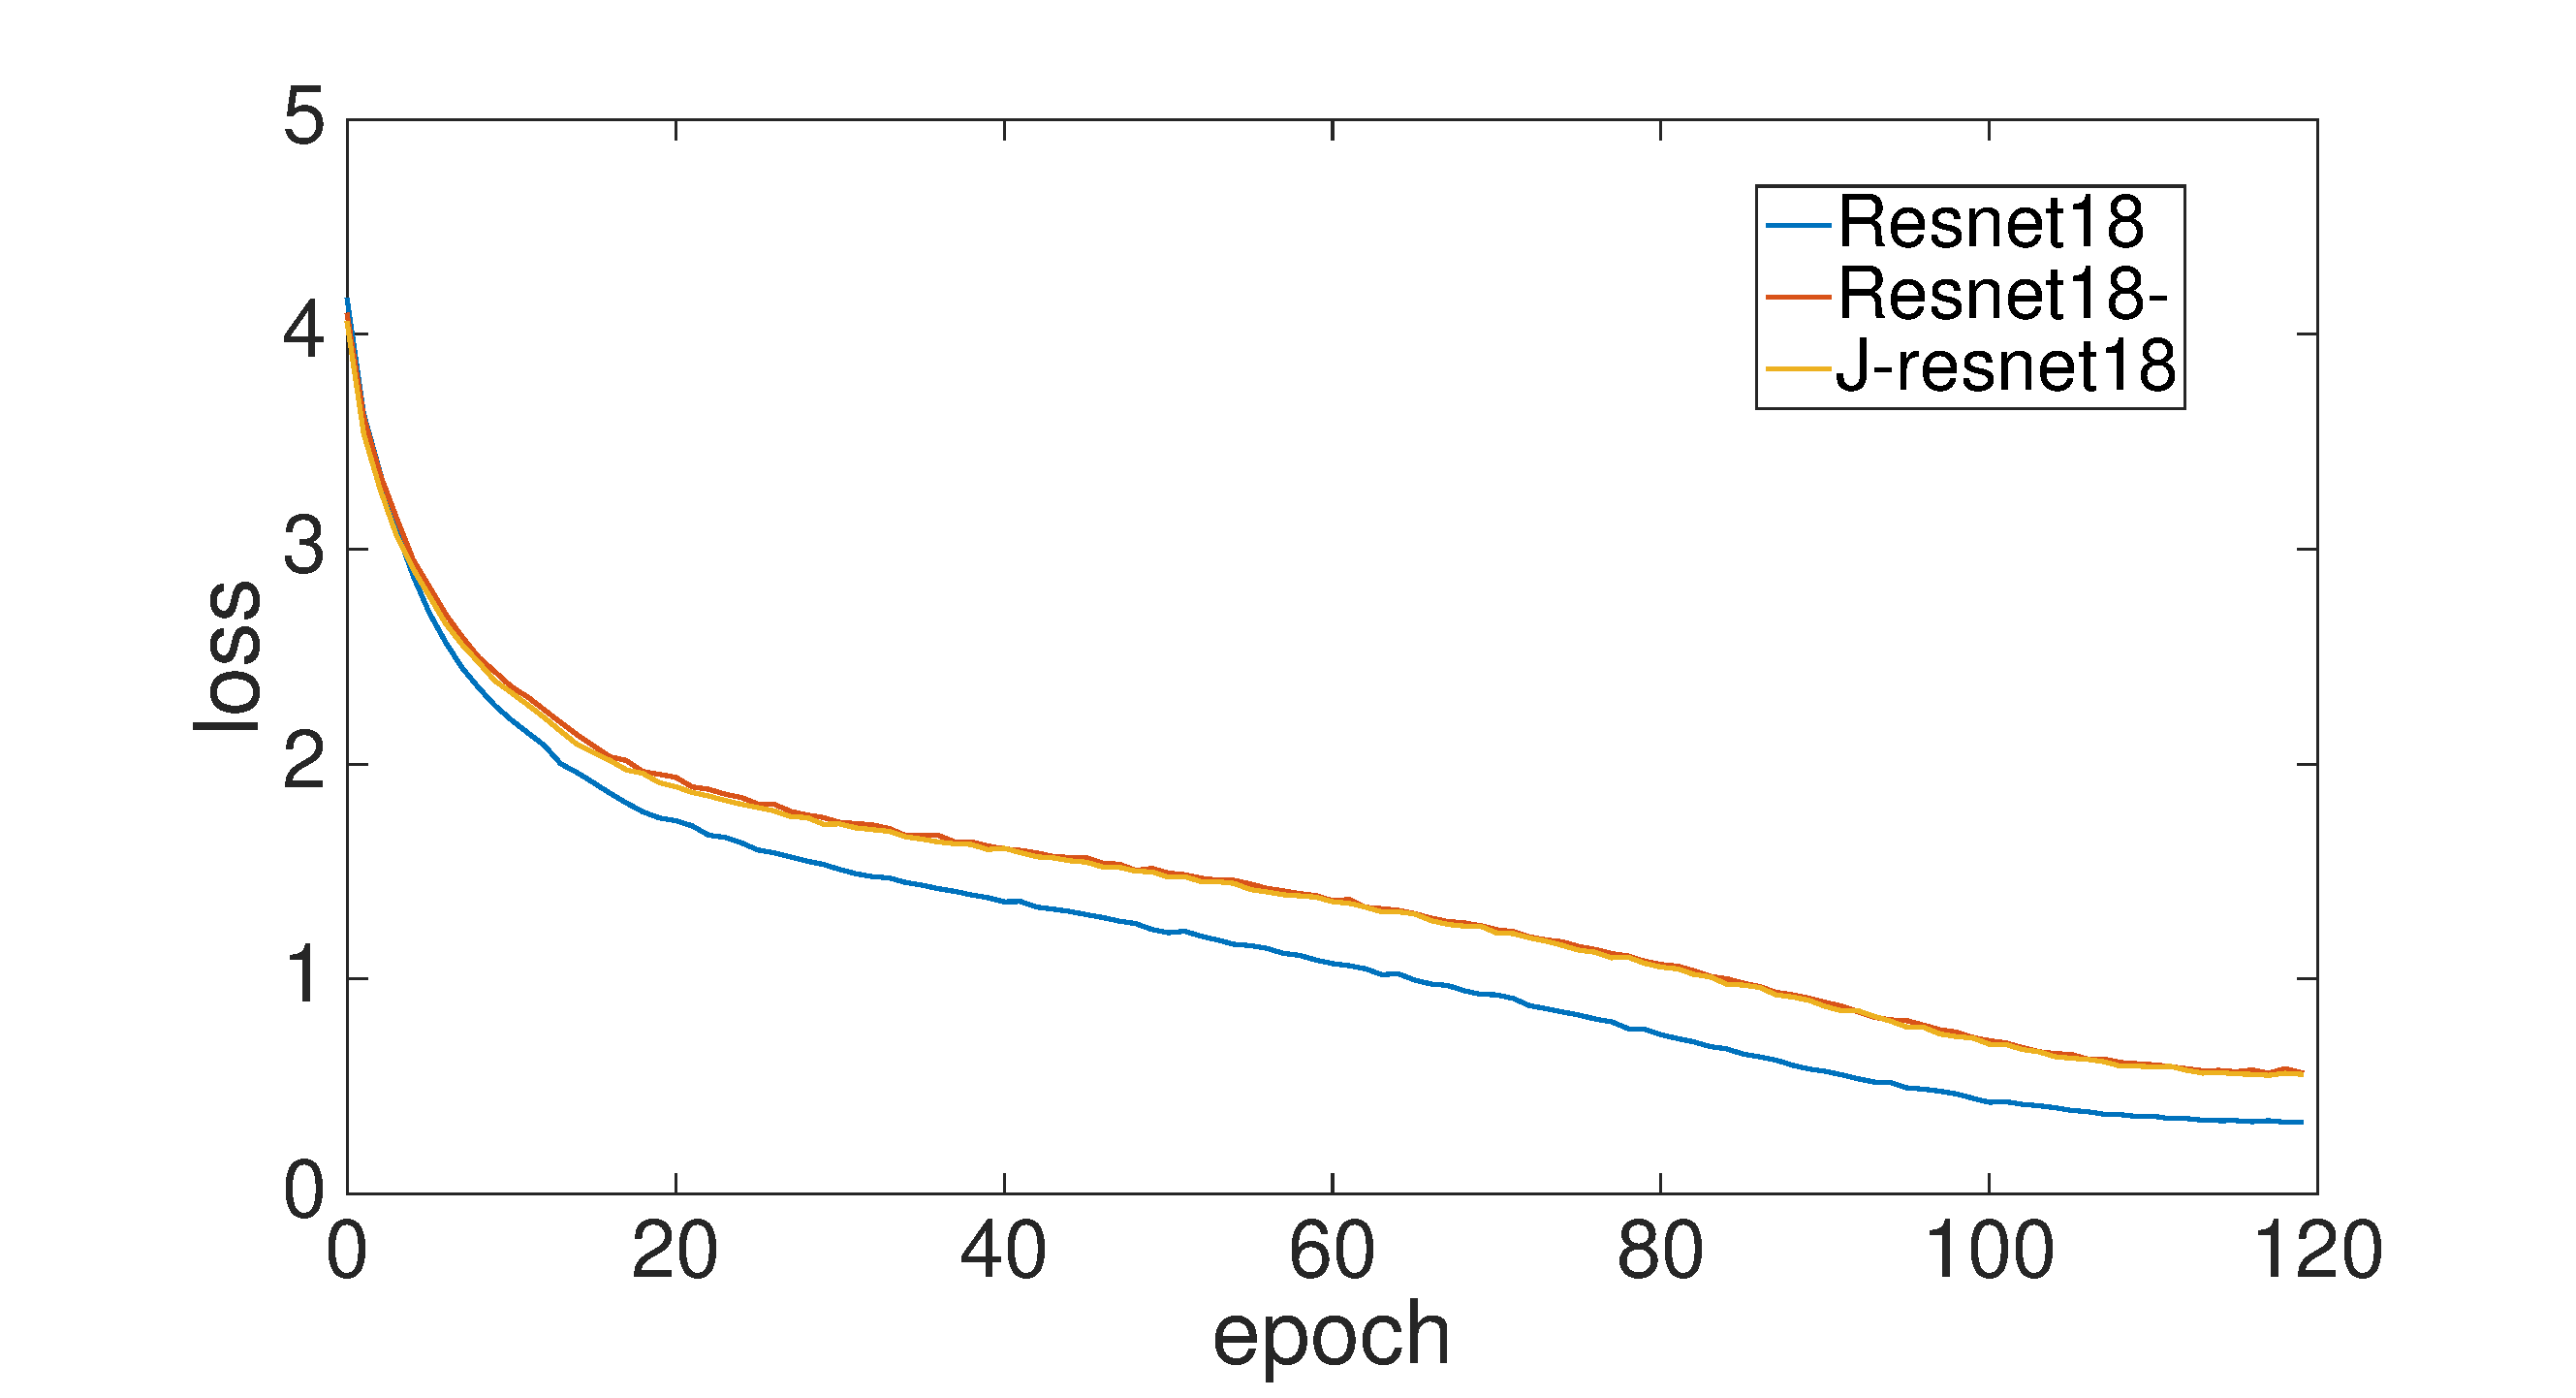
\includegraphics[width=0.45\textwidth]{figures/Jresnet/FIG7(a)_TII-21-2603.eps}
		\label{a}
	}
	\subfigure[resnet18的验证误差]{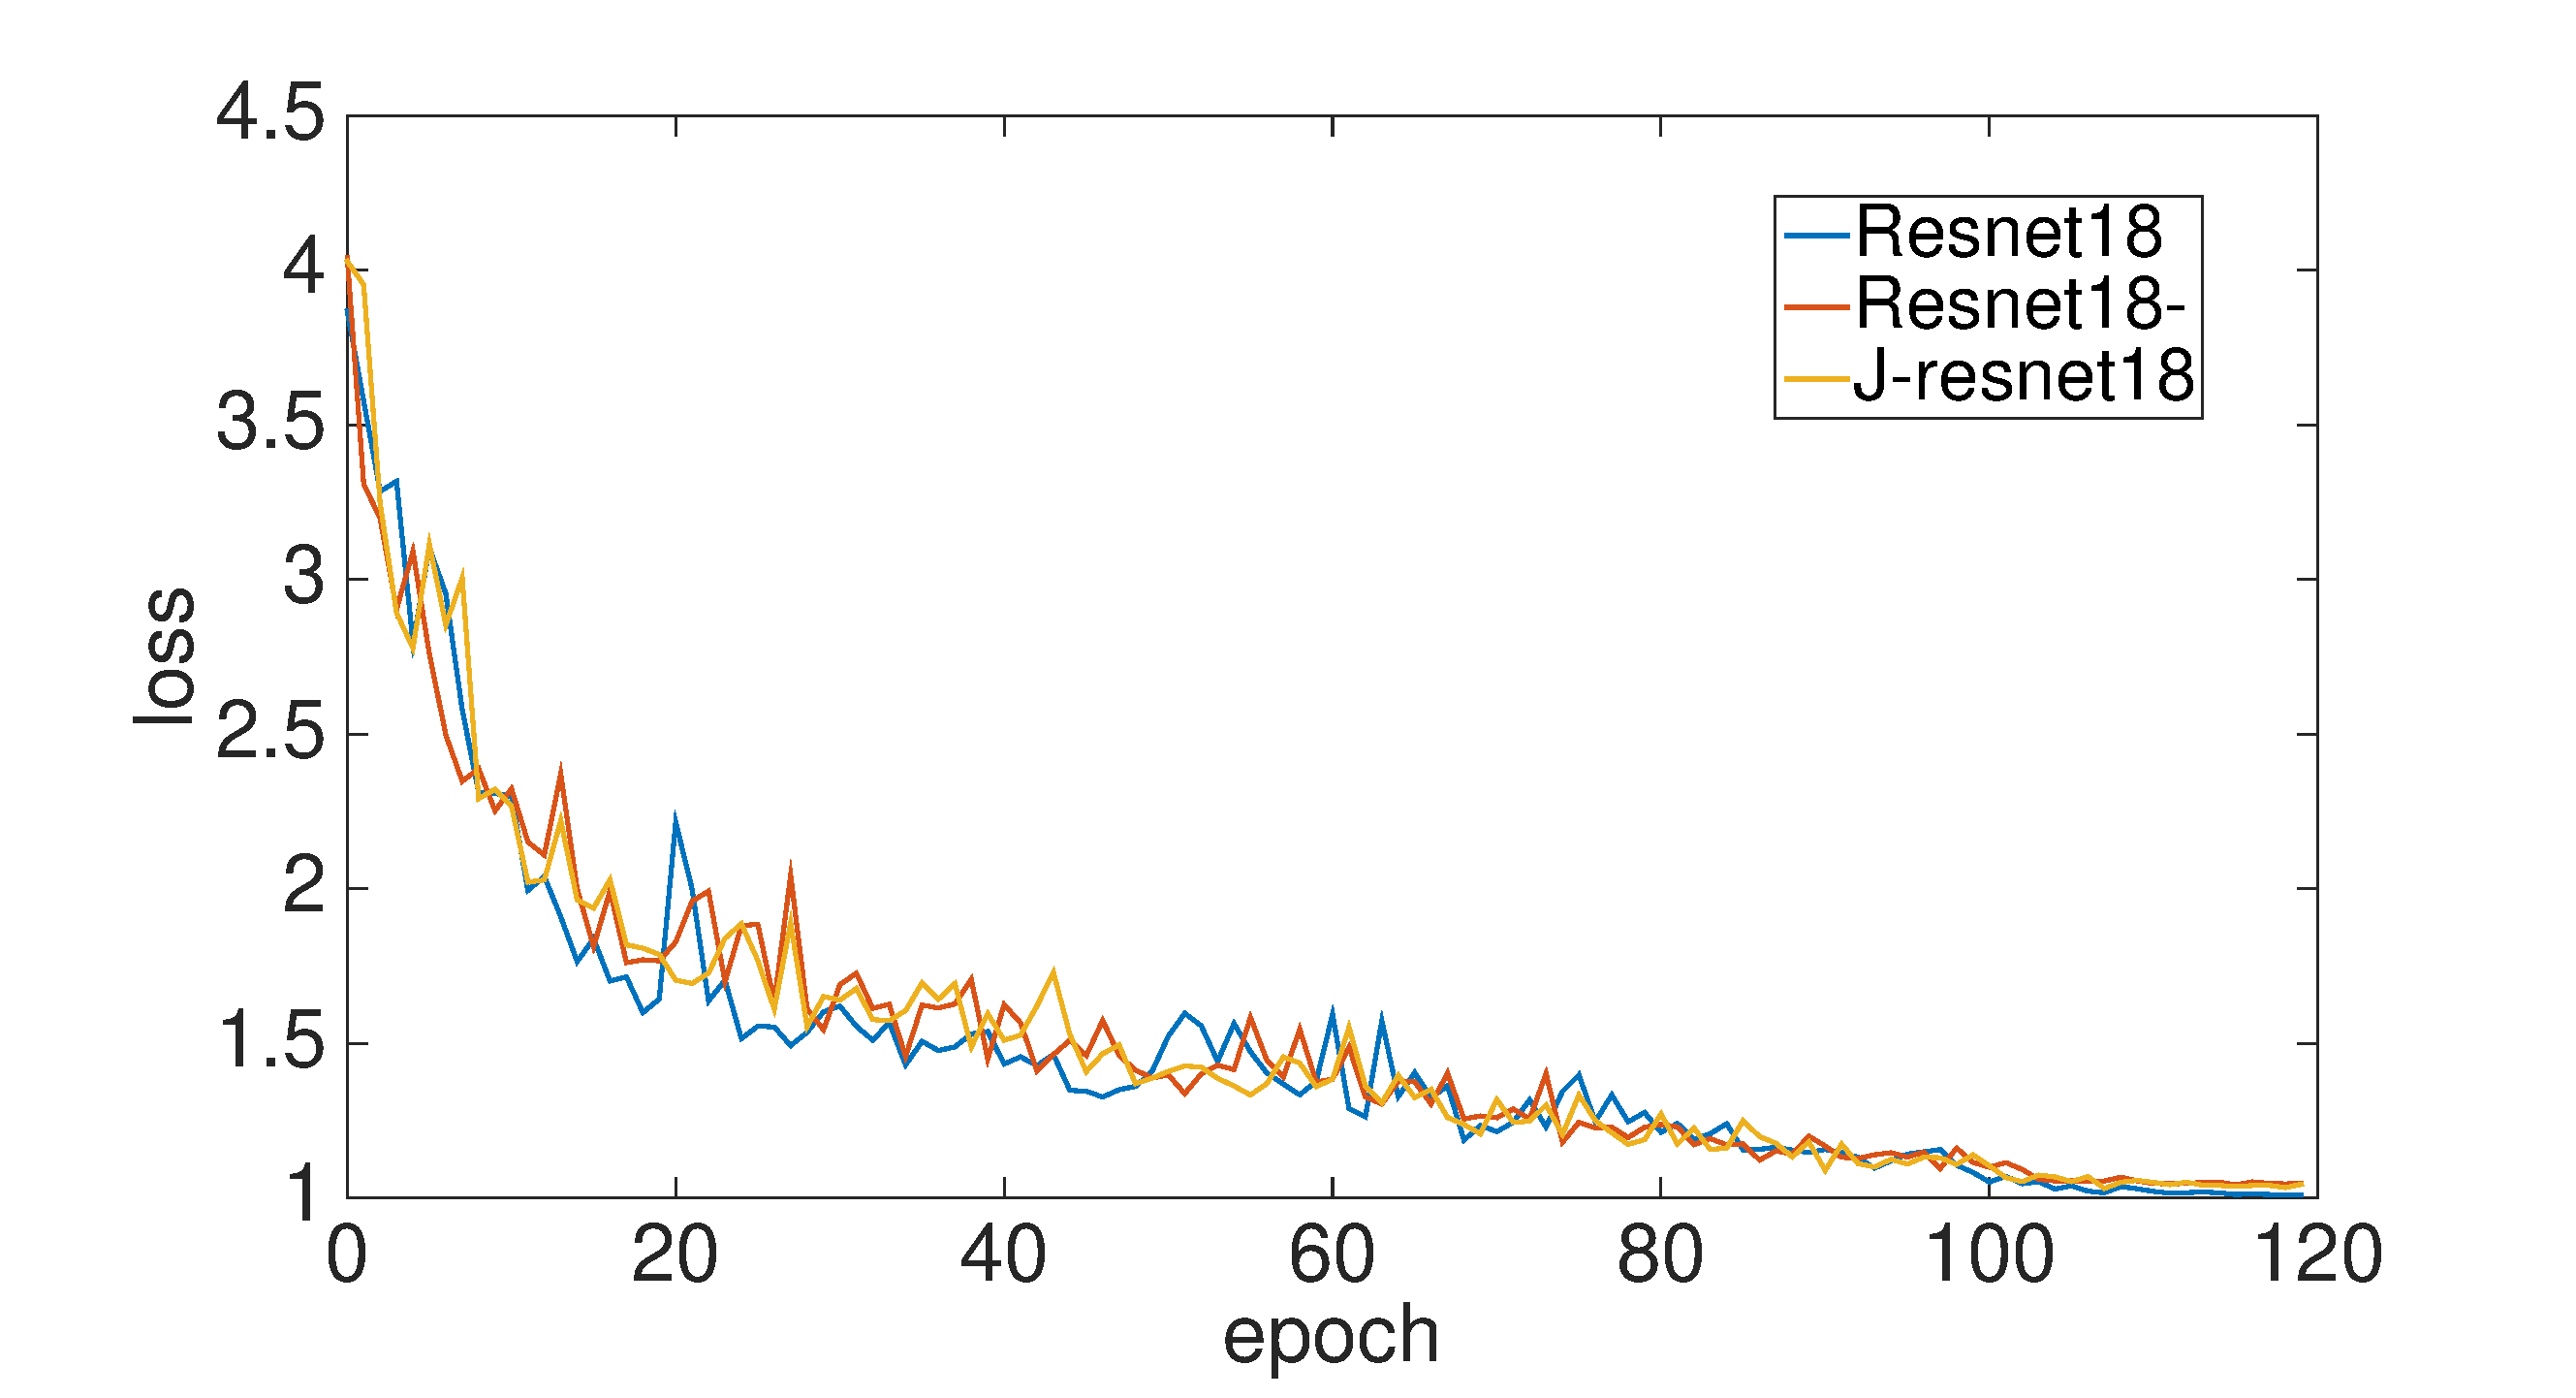
\includegraphics[width=0.45\textwidth]{figures/Jresnet/FIG7(b)_TII-21-2603.eps}
		\label{b}}
	
	\subfigure[resnet18的训练准确率]{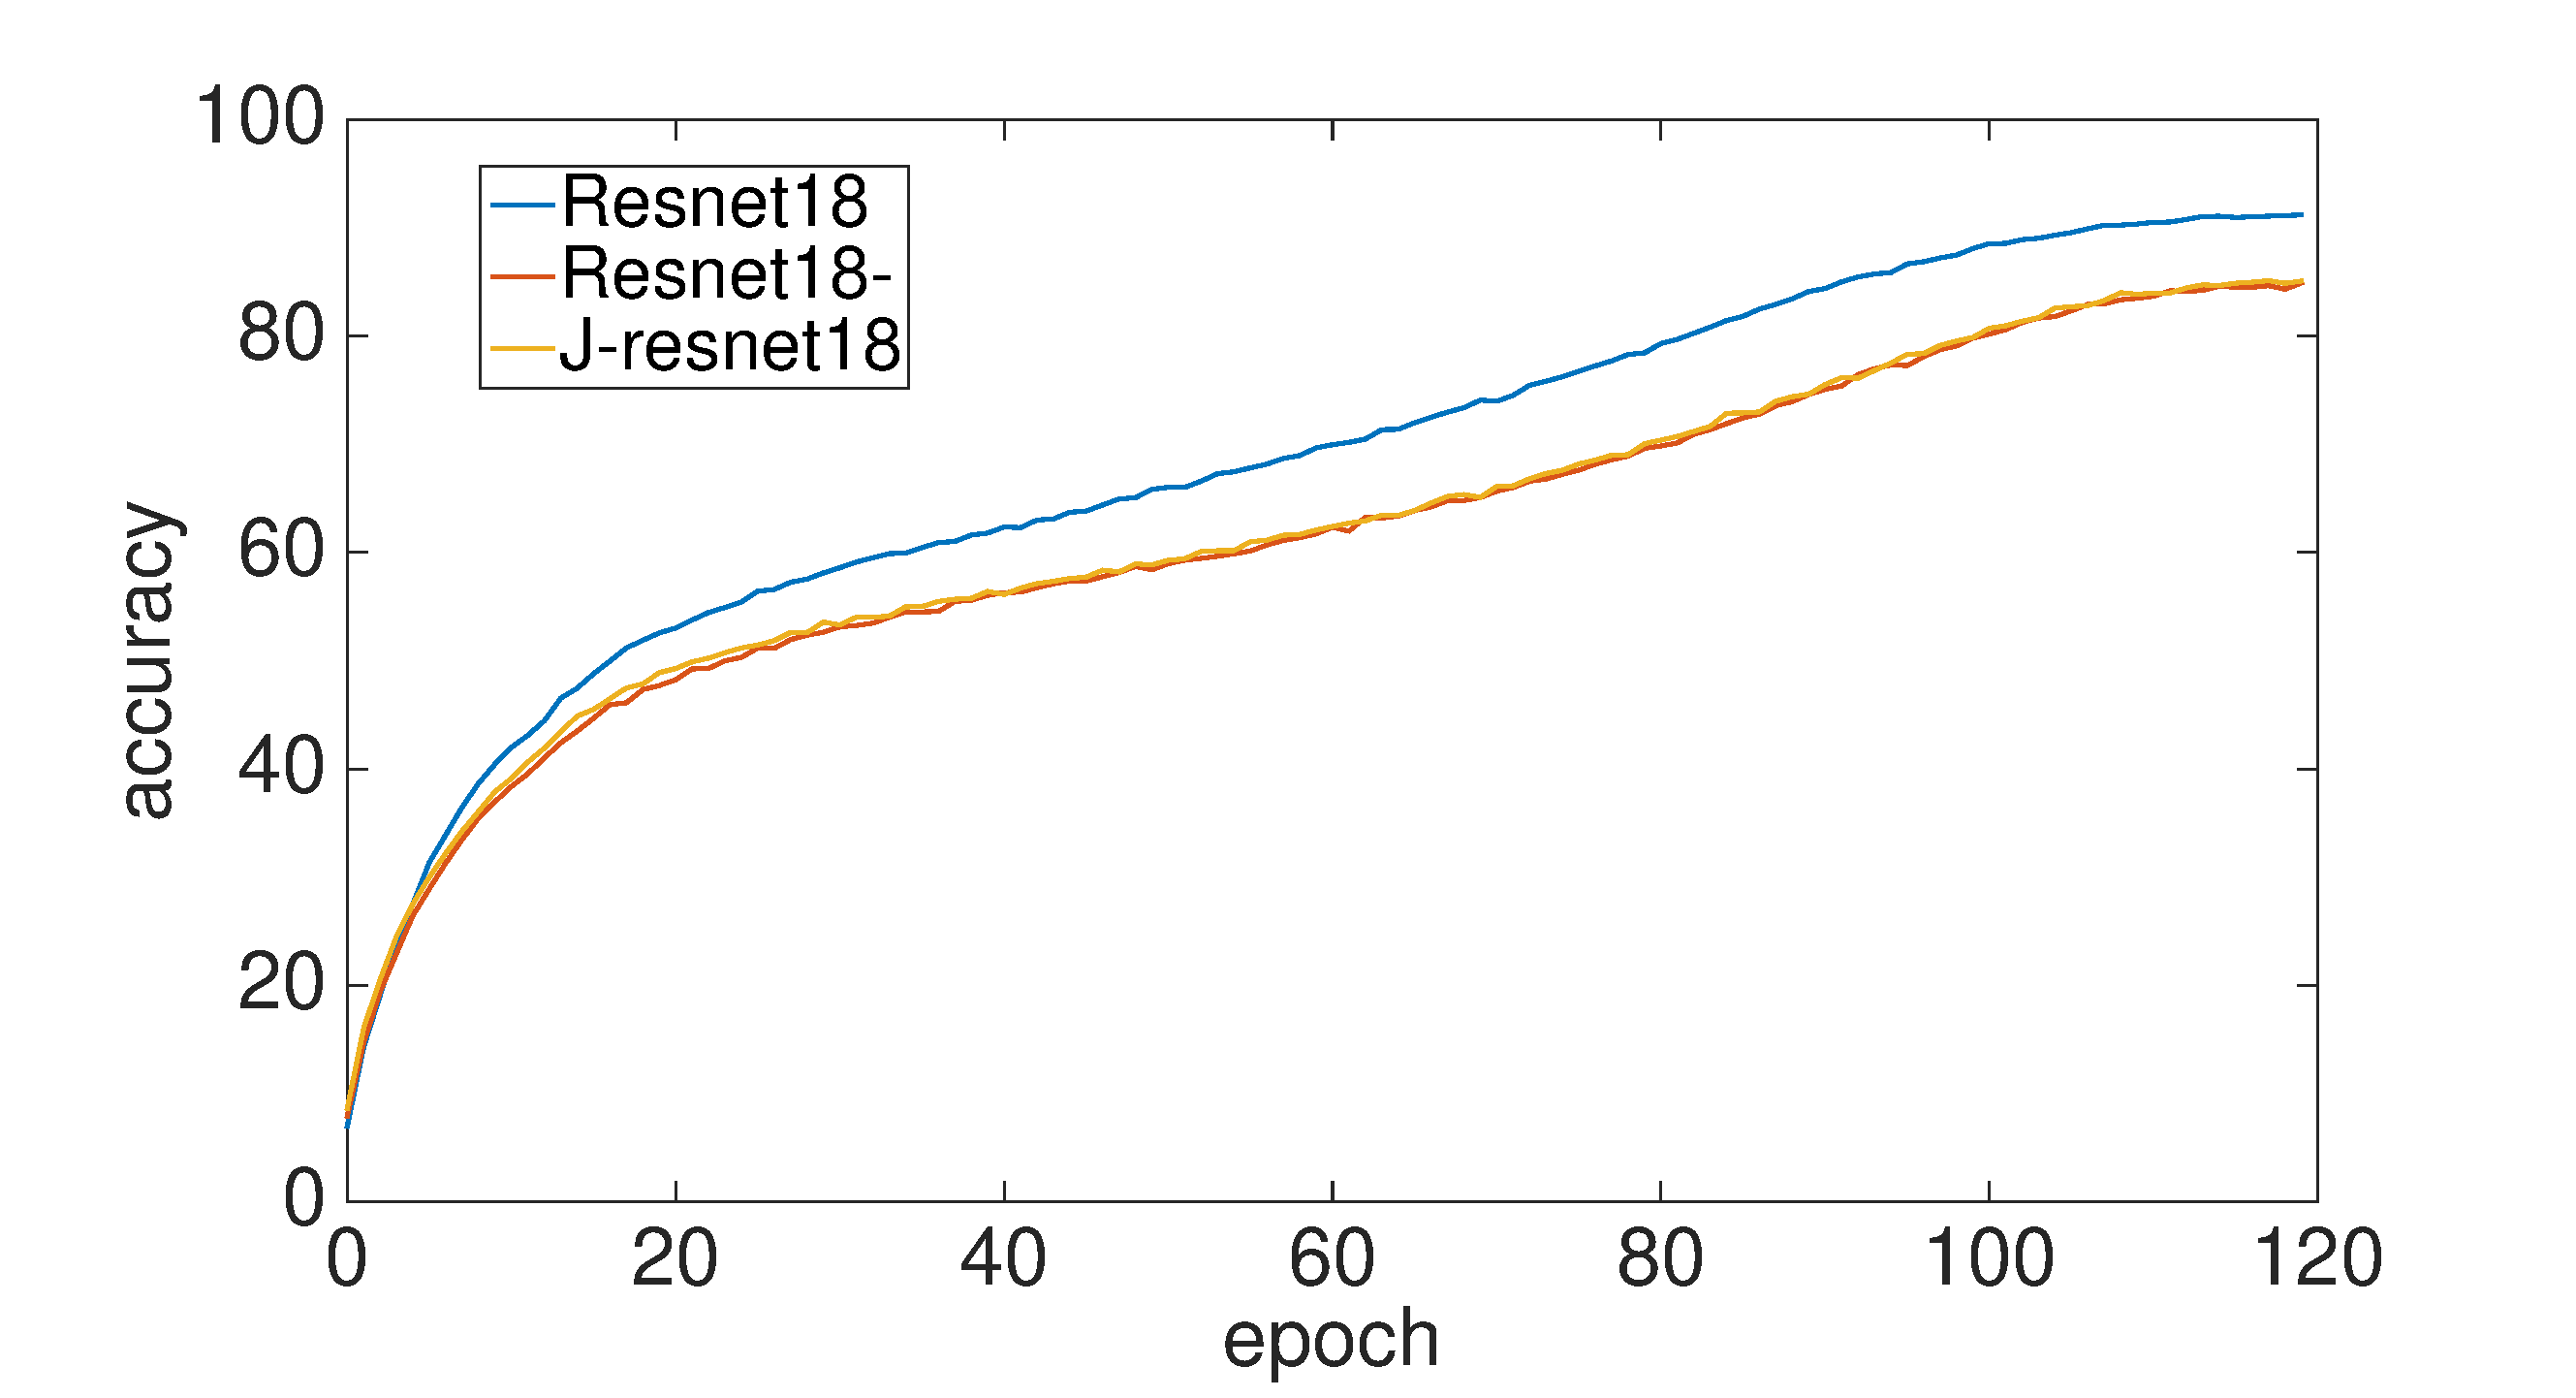
\includegraphics[width=0.45\textwidth]{figures/Jresnet/FIG7(c)_TII-21-2603.eps}
		\label{c}}
	\subfigure[resnet18的验证准确率]{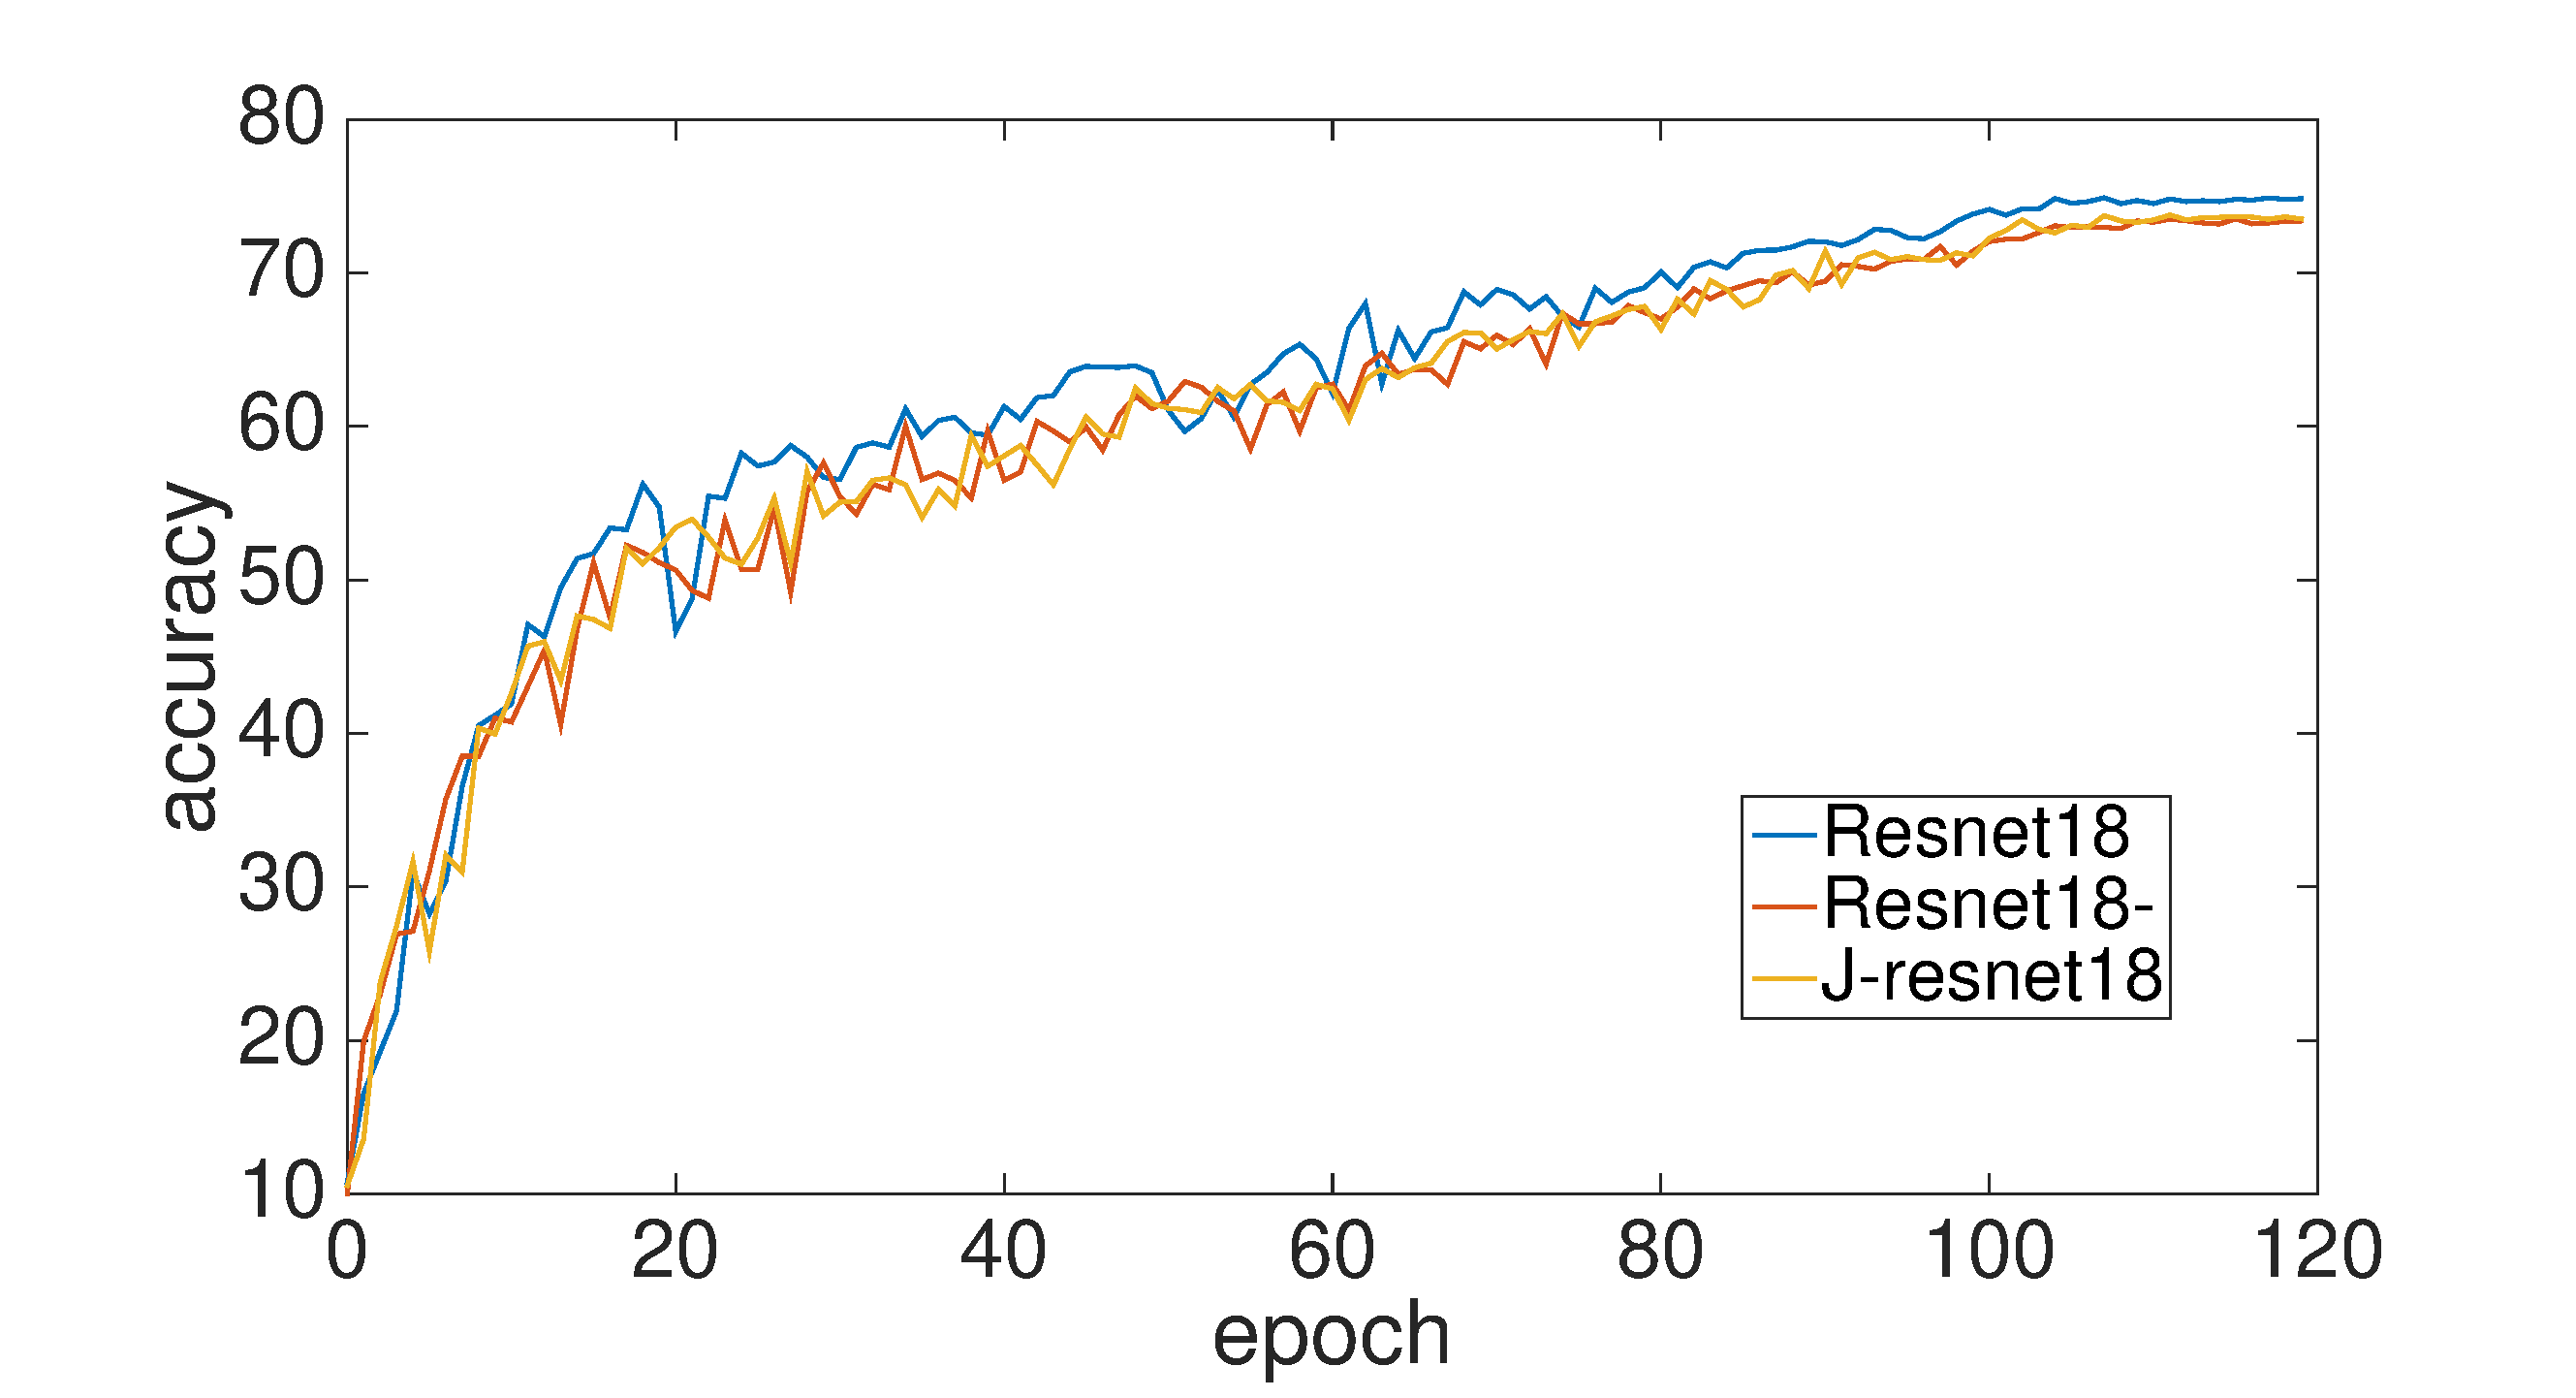
\includegraphics[width=0.45\textwidth]{figures/Jresnet/FIG7(d)_TII-21-2603.eps}
		\label{d}}
	
	\hfil
	
	\subfigure[resnet50的训练误差]{
		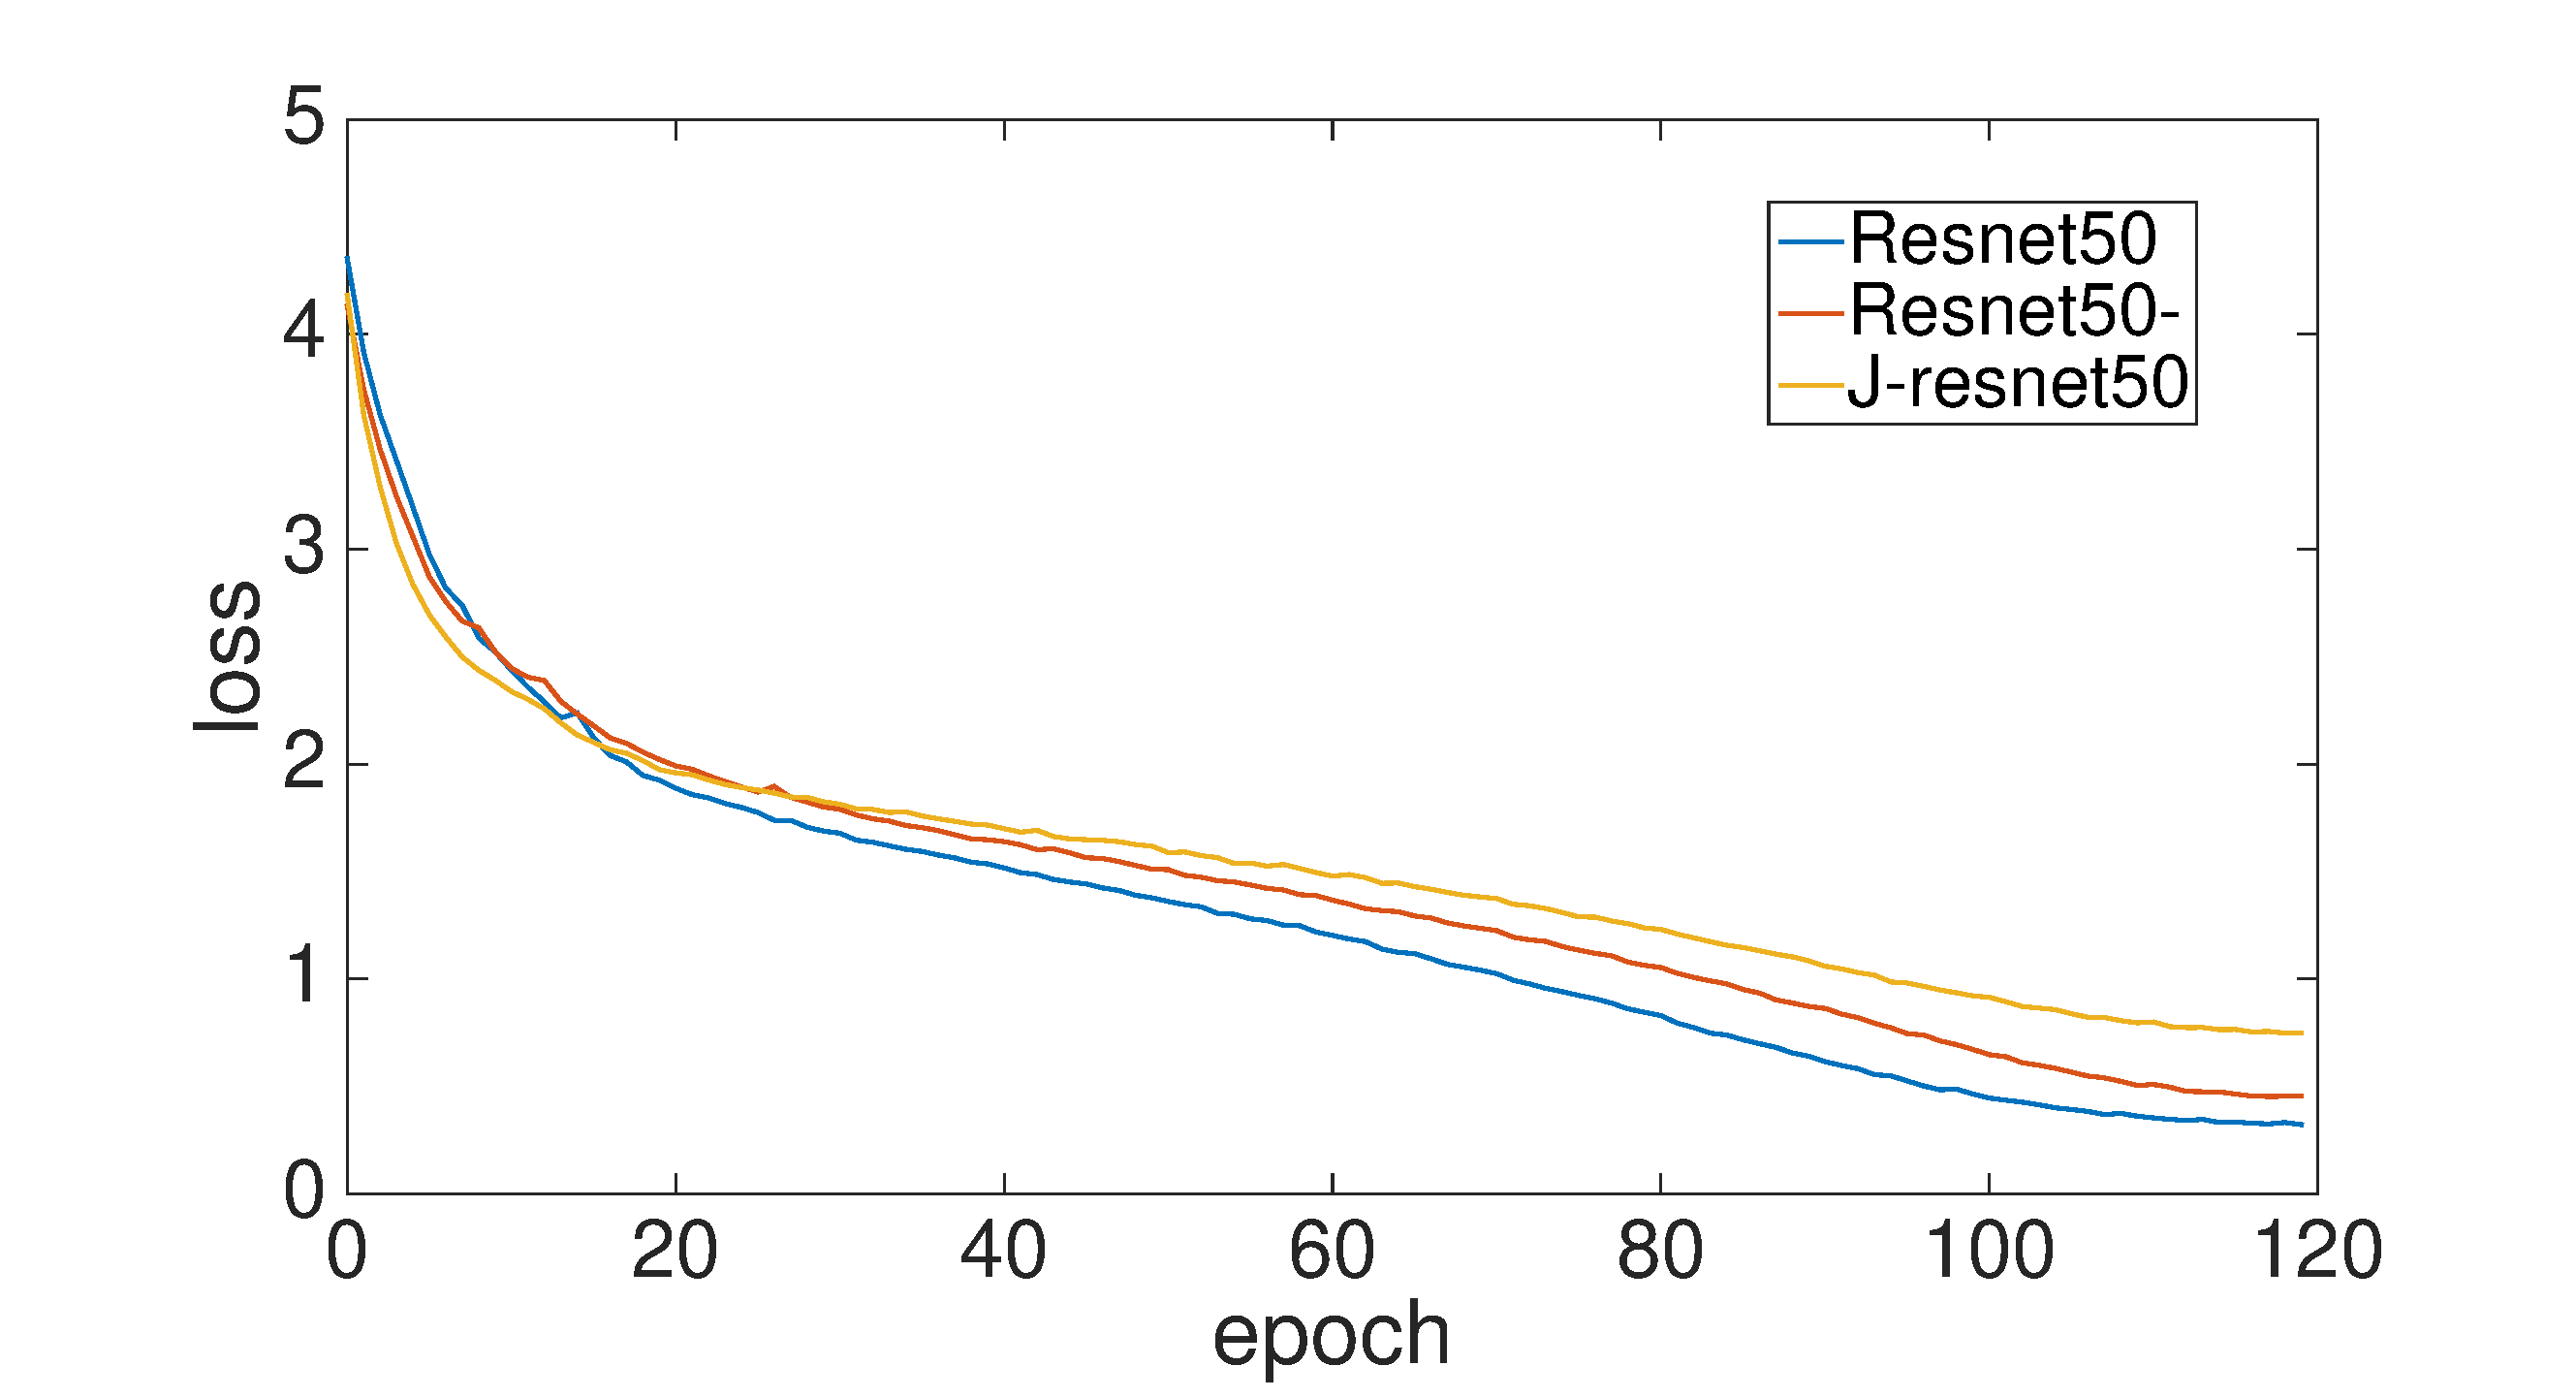
\includegraphics[width=0.45\textwidth]{figures/Jresnet/FIG7(e)_TII-21-2603.eps}
		\label{e}
	}
	\subfigure[resnet50的验证误差]{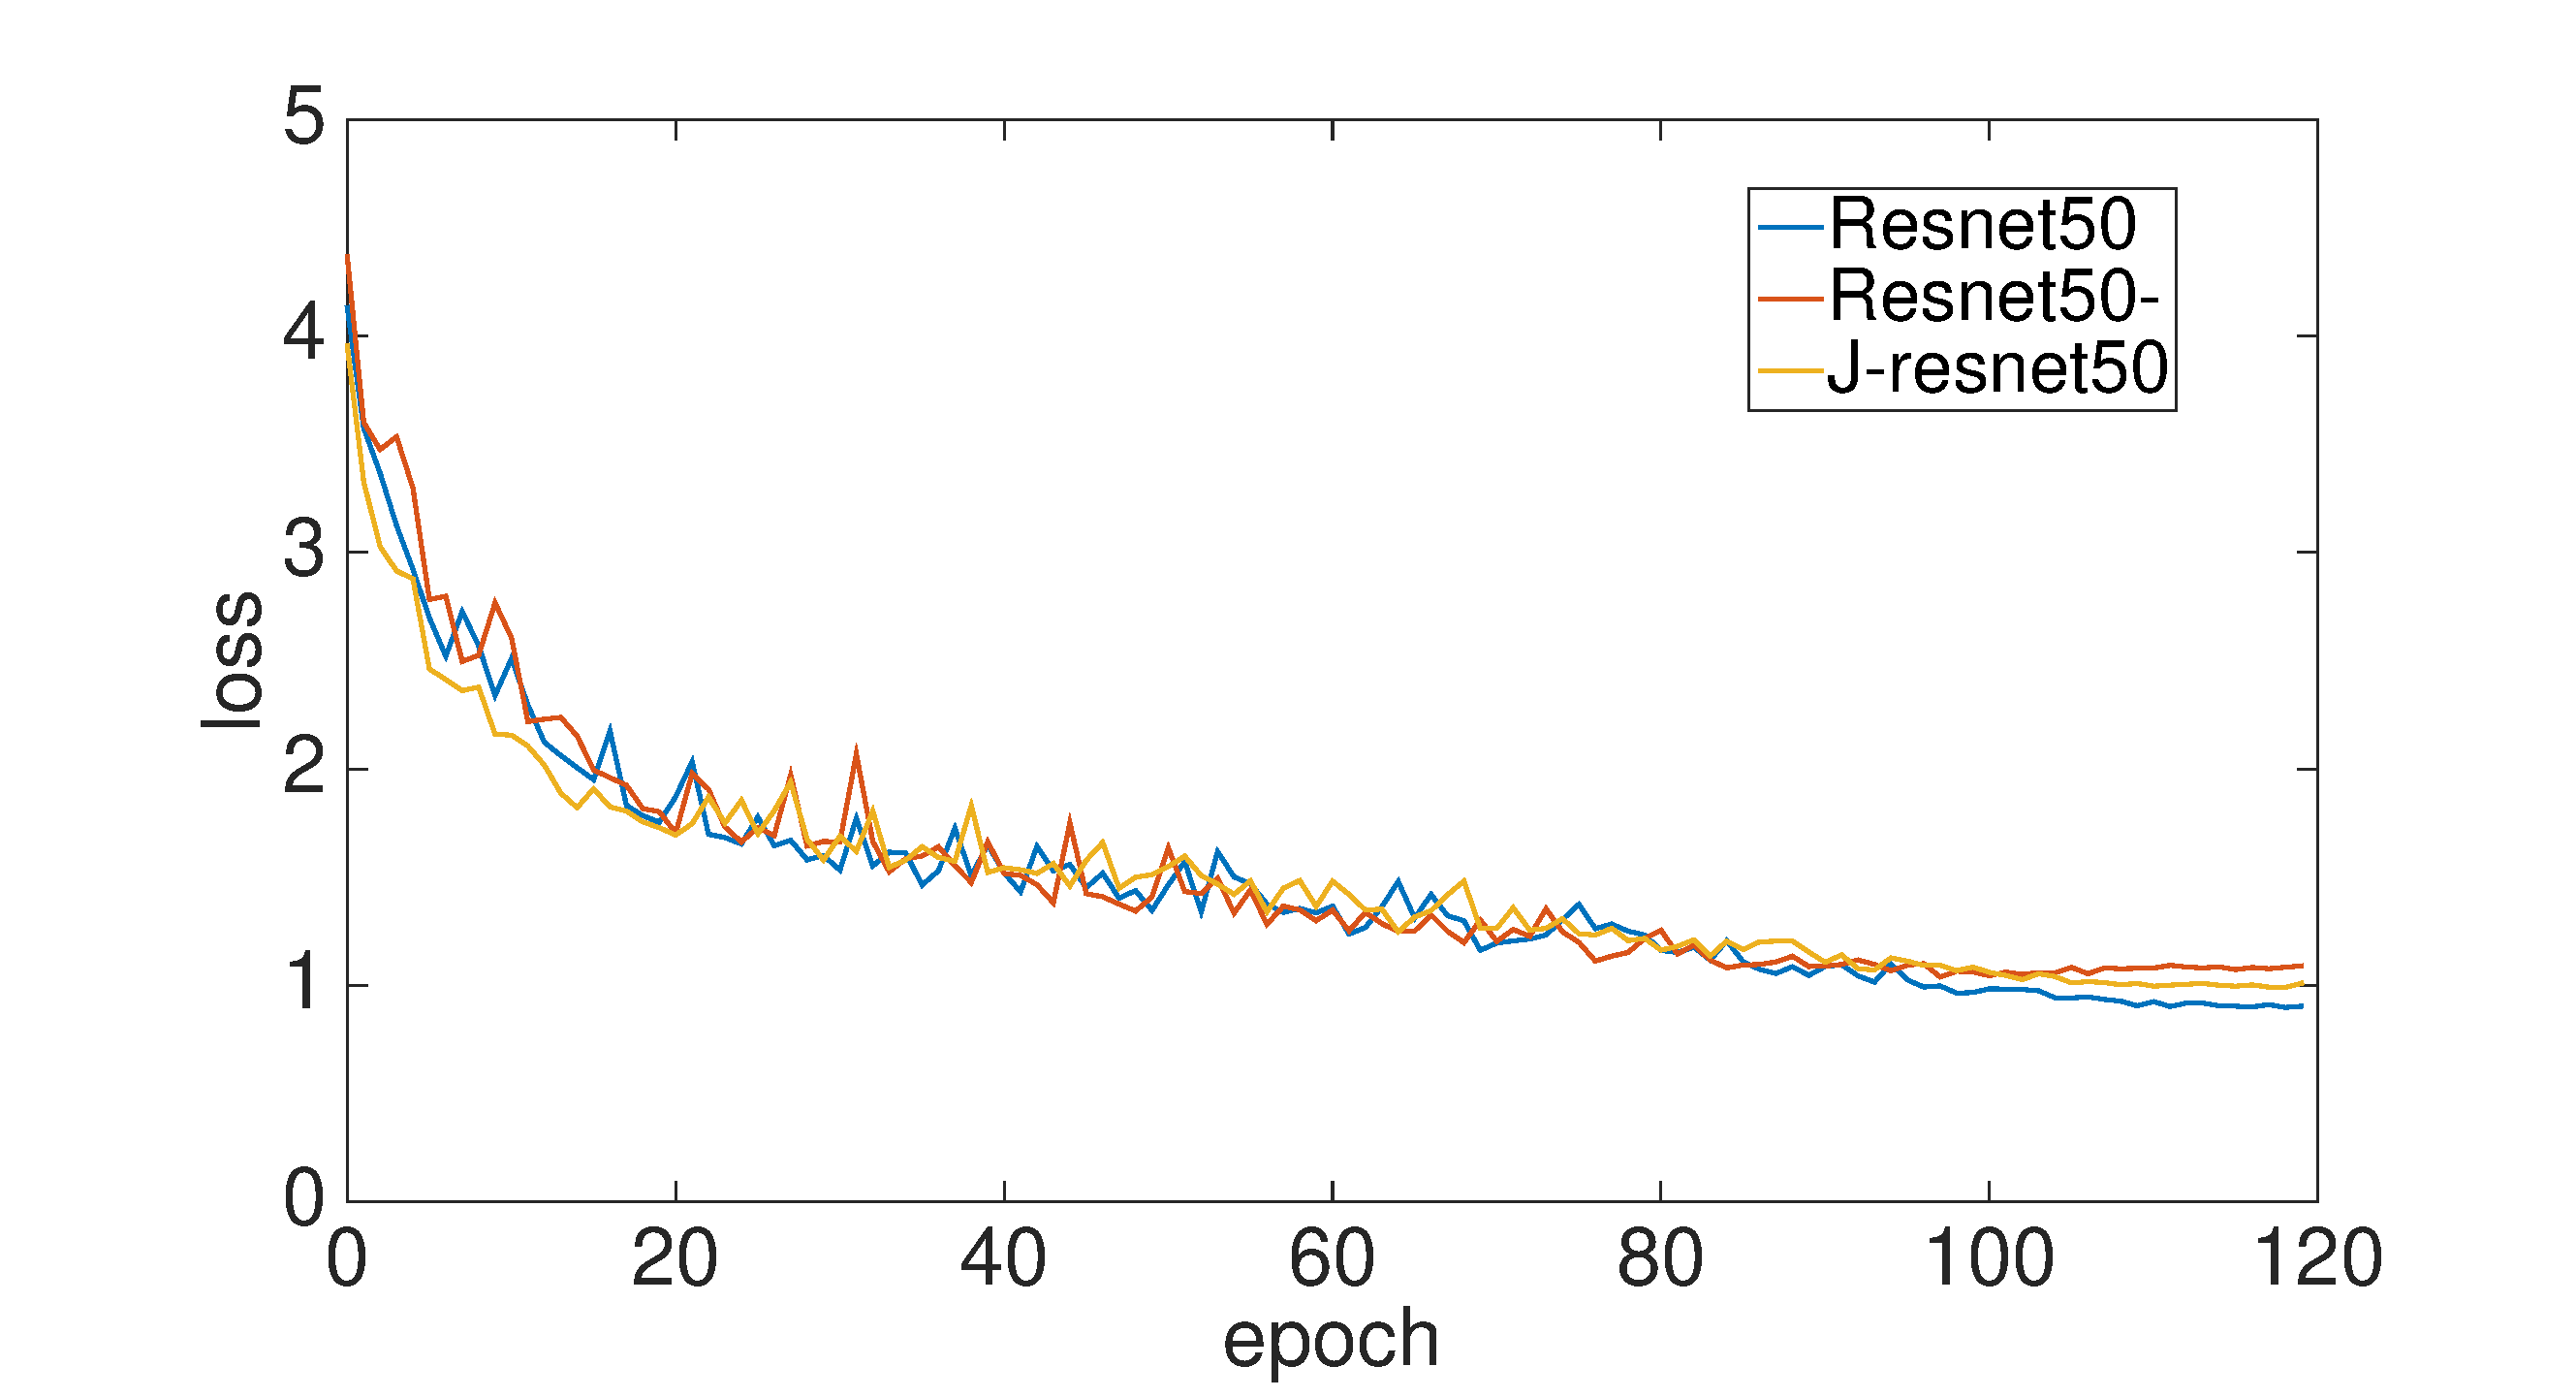
\includegraphics[width=0.45\textwidth]{figures/Jresnet/FIG7(f)_TII-21-2603.eps}
		\label{f}}
	
	\subfigure[resnet50的训练误差]{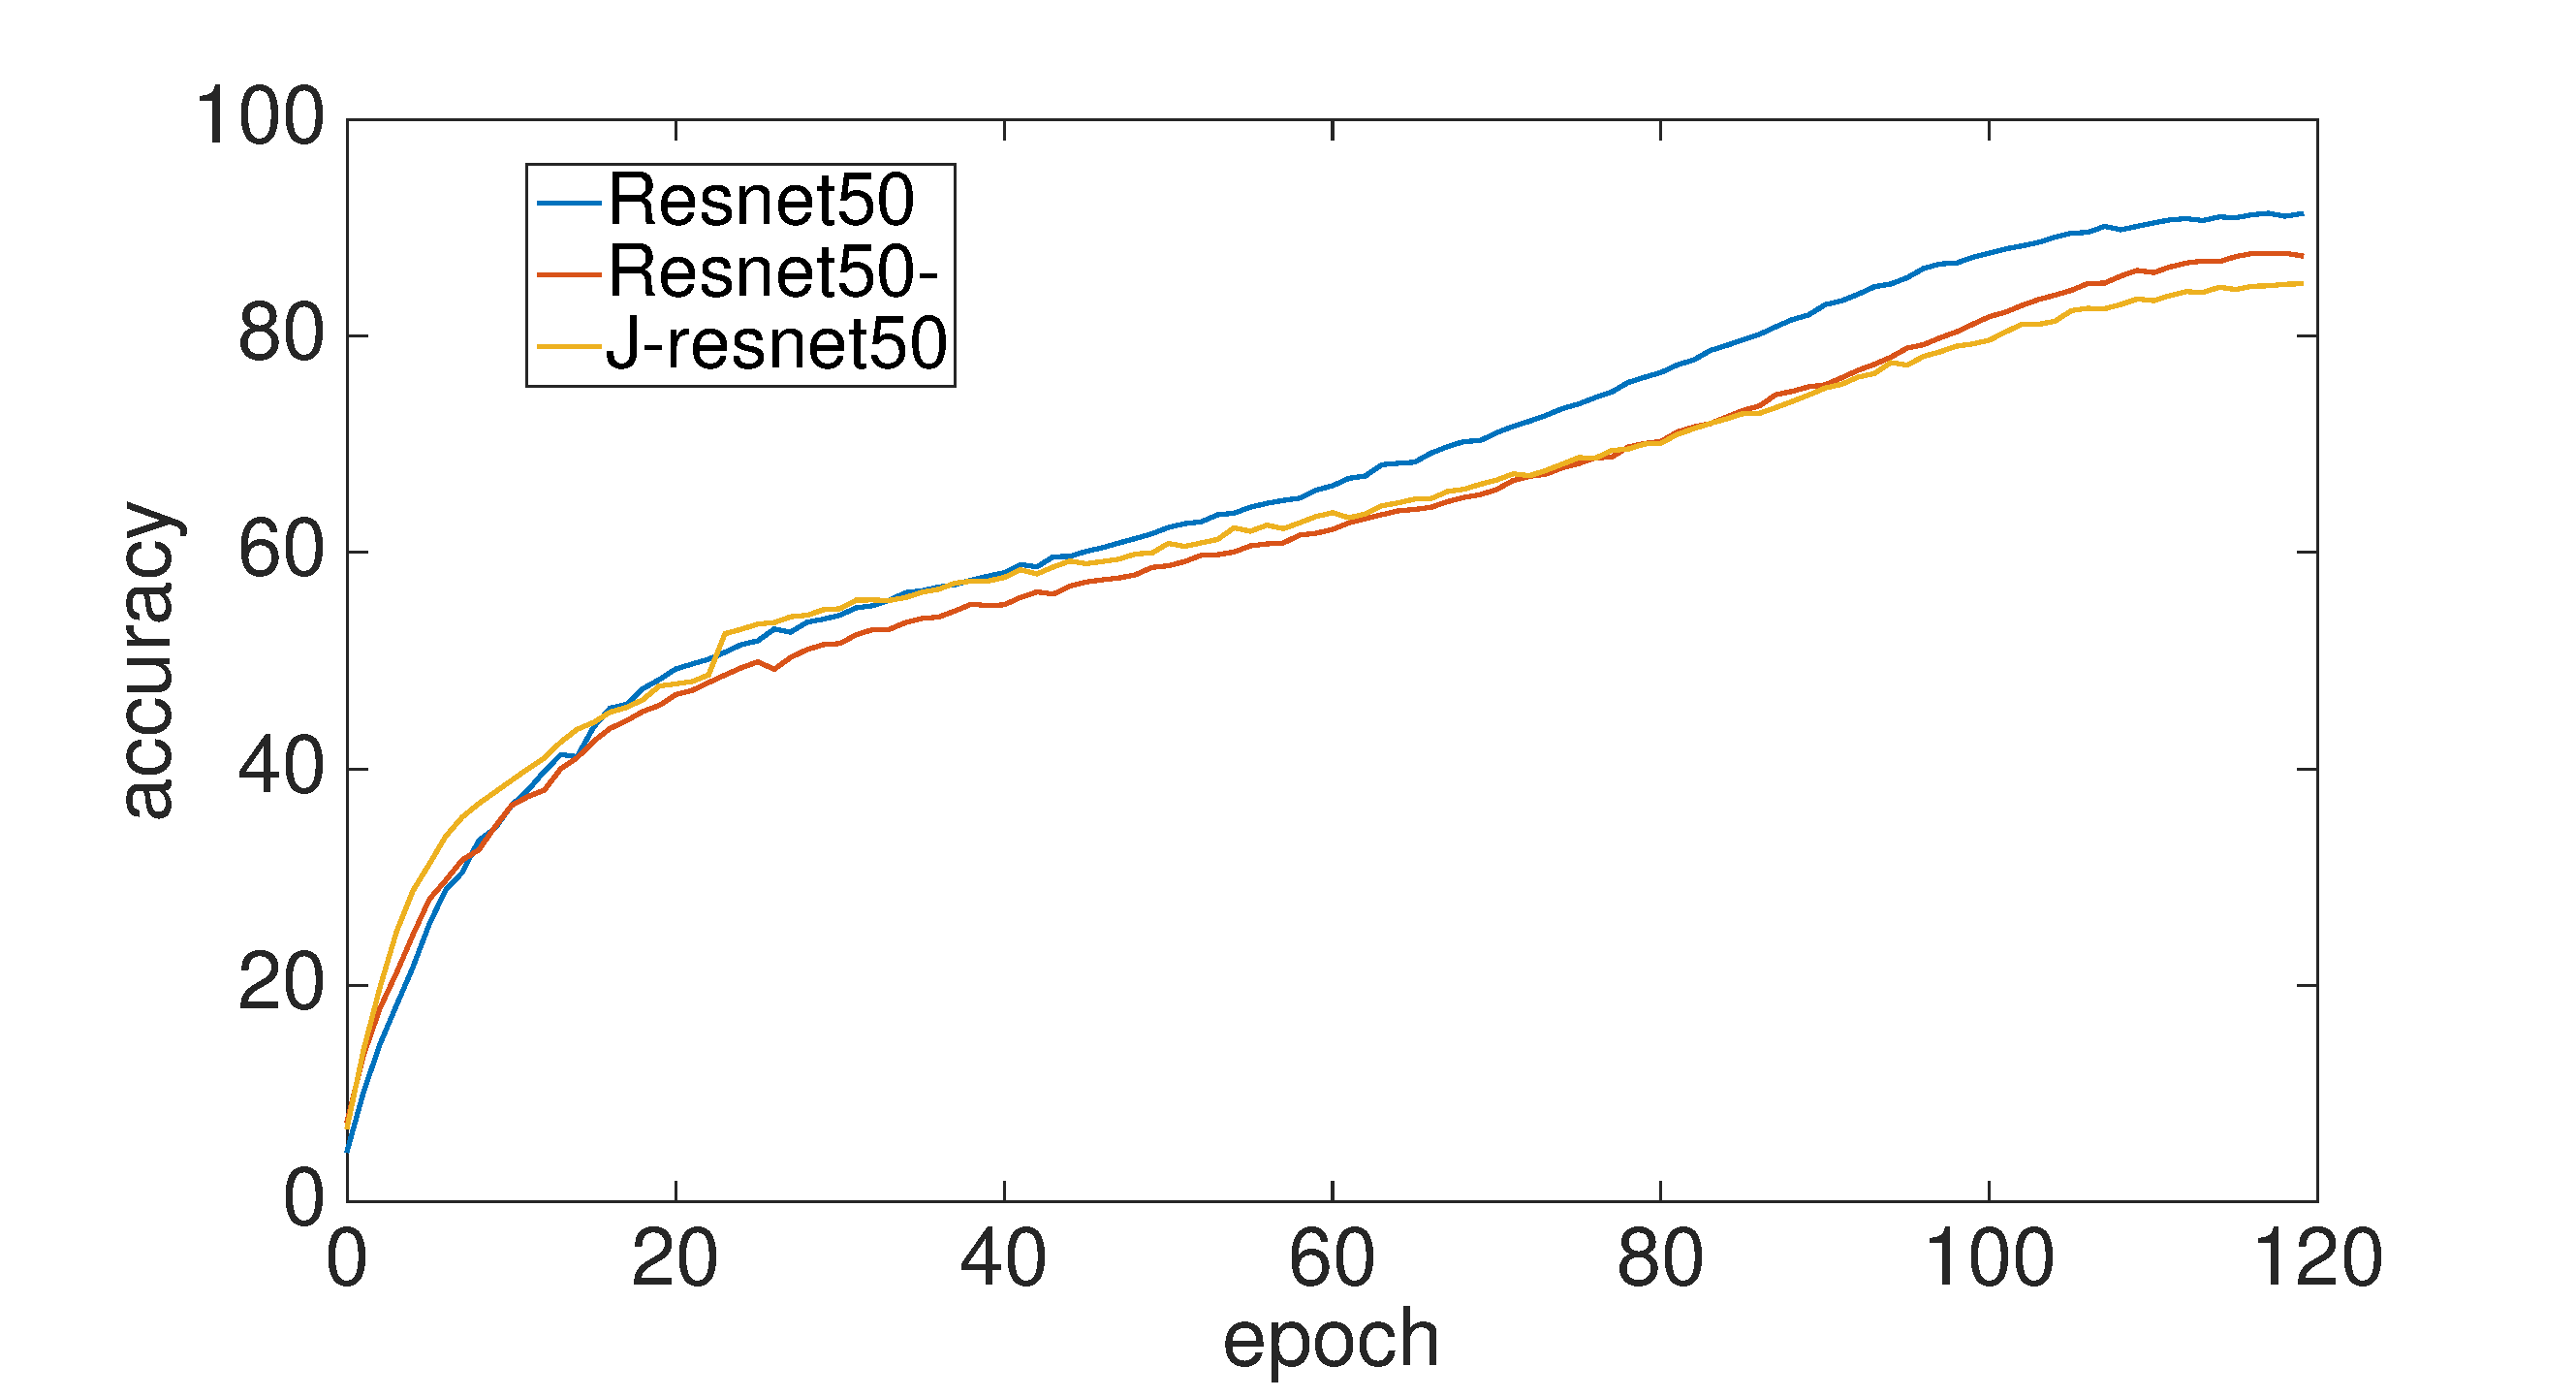
\includegraphics[width=0.45\textwidth]{figures/Jresnet/FIG7(g)_TII-21-2603.eps}
		\label{g}}
	\subfigure[resnet50的验证准确率]{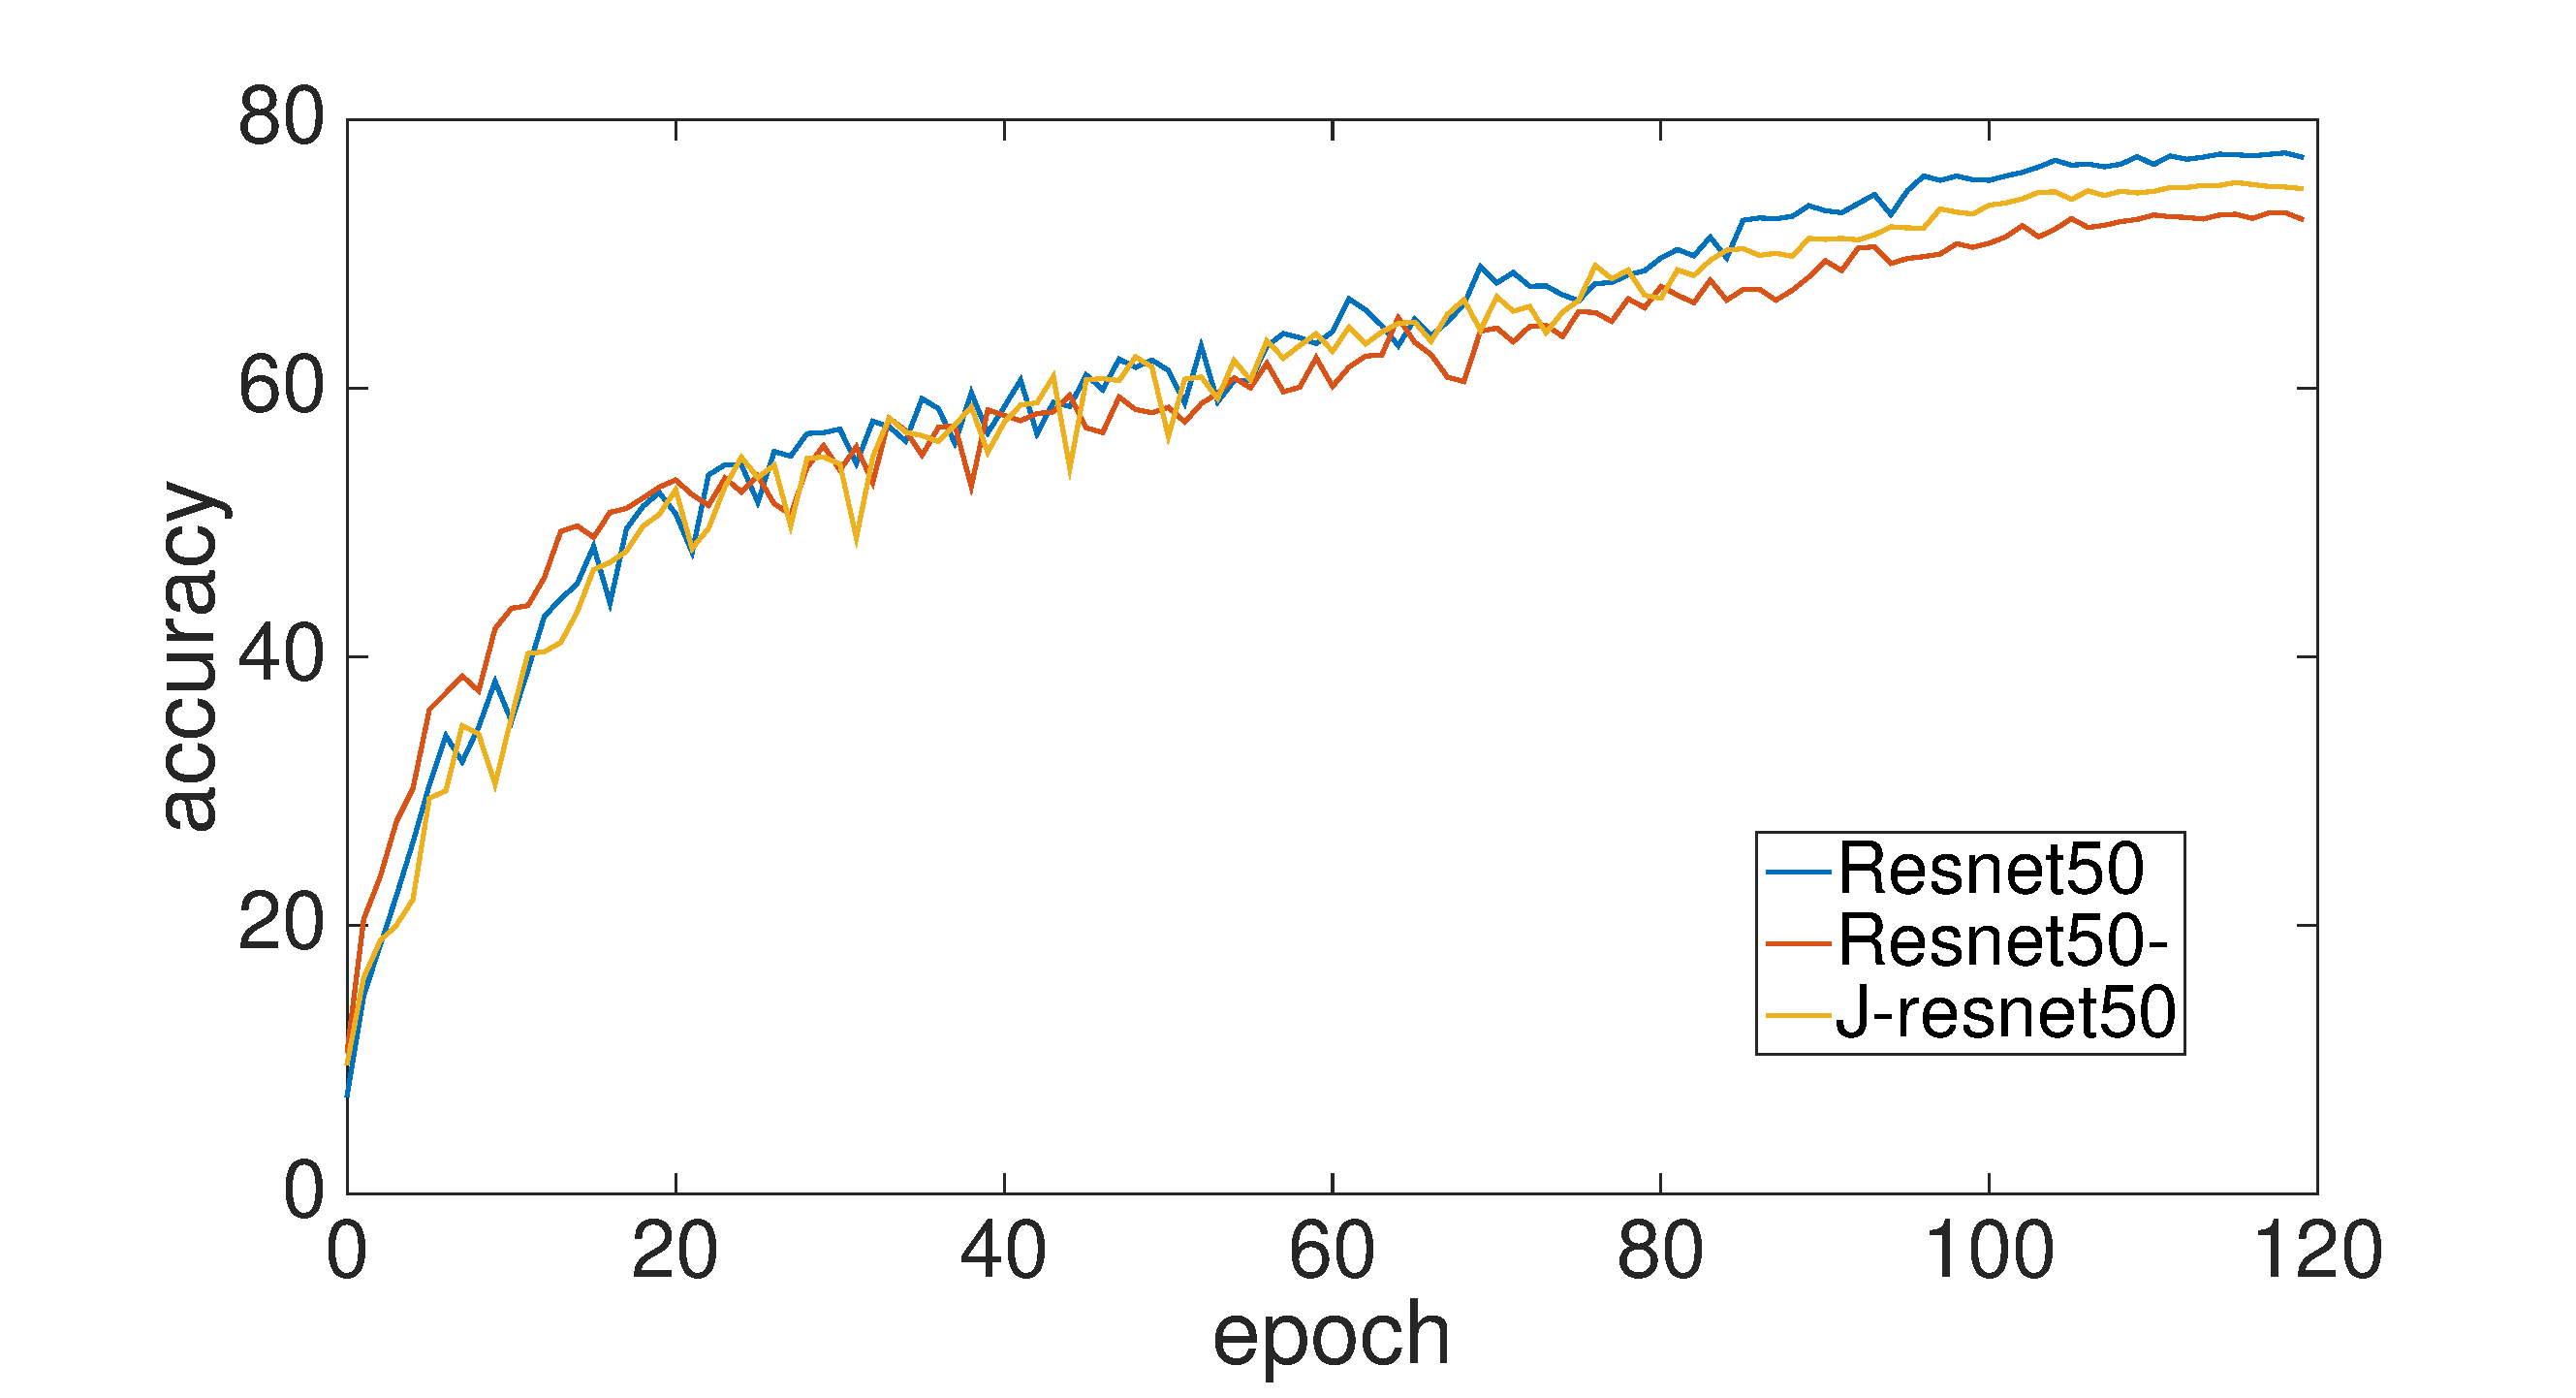
\includegraphics[width=0.45\textwidth]{figures/Jresnet/FIG7(h)_TII-21-2603.eps}
		\label{h}}
	
	\caption{
		Resnet和Juggler Resnet在\emph{CIFAR-100}数据集上,以学习率=0.1、批量大小=256、动量系数=0.9的标准SGD,在5个epoch余弦退火的预热后,120个epoch的实验训练结果。\emph{J-resnet$_i$}表示不同深度的Juggler-Resnet,\emph{Resnet$_i$-} \emph{resnets} 表示两个相邻卷积核之间没有relu层插入的网络。 Train loss和 validate loss分别是在训练集和验证集上的误差。}
	\label{train_results}
\end{figure*}

\subsection{实验结果}
\subsubsection{训练表现}
图\ref{train_results}(a),(b),(e),(f)的训练结果表明,Juggler-ResNet可以应用于不同深度的\emph{ResNet},并且收敛速度几乎相同。图 \ref{train_results}(c),(g),(d),(h) 表明Juggler-ResNet的图片分类准确度略有下降,比原来的\emph{ResNet}低约1.4\%-1.79\%。\emph{这种精度下降可以通过增强训练数据来解决,这超出了本文的讨论范围}. 此外,与没有relu层的\emph{ResNet}相比,Juggler-ResNet的图片分类精度大约高出0.7\%-0.9\%百分点(即 在图中用'-'标识出来的)。这表明,在3x3卷积核处加宽通道数可以减少因移除relu层而导致的精度降低问题。值得注意的是,在相同训练次数的参数设置下,\emph{resnet}在训练集上比Juggler-ResNet获得更高的准确率,在\emph{resnet18}上高6.11\%,在\emph{resnet50}上高12.03\%。训练集和验证集之间的这一巨大精度差距表明,在相同的训练次数设置下,Juggler-ResNet比\emph{ResNet}具有更好的泛化能力。

为了进一步验证Juggler ResNet在不同数据集和不同深度的\emph{ResNet}上的图片分类准确率性能,我们比较了Juggler-ResNet和\emph{ResNet}在不同深度范围 (从\emph{resnet18}到\emph{resnet152})上的图片分类准确率。表\ref{Cifar10_Cifar100}显示图片分类精度随深度的增加而降低。Juggler-ResNet和\emph{ResNet}之间的精度差距在\emph{resnet152}达到最大值,在CIFAR-10数据集上约为1.41\%,在CIFAR-100数据集上约为1.91\%。Juggler-ResNet的优异性能来自以下贡献。1)随着深度的增加,relu层可以通过将部分参数设置为零来减少参数之间的依赖性。2) CIFAR-100数据集的分类类别比CIFAR-10数据集更复杂。然而,Juggler-ResNet在CIFAR-10和CIFAR-100数据集上的平均性能仍然优于其他基于线性拓扑结构的模型,如vgg和alexnet,图片分类准确率分别高出10.9\%和39.78\%。结果表明,与基于线性拓扑结构的模型相比,Juggler-ResNet保留了多分支结构的特征提取能力,达到了SOTA级别的图片分类精度性能。
\begin{table}[h]
	\caption{The comparison results on \emph{Cifar10} and \emph{Cifar100} trained in 120 epochs. The \emph{Acc1} denotes the top-1 accuracy on validate dataset.}
	\label{Cifar10_Cifar100}
	\centering
	\begin{tabular}{lcccc}
		\hline
		\textbf{Model} & \textbf{CIFAR-10 Acc1}  &\textbf{\ Gap} & \textbf{CIFAR-100 Acc1}  &\textbf{\ Gap} \\
		\hline
		Resnet18   & 94.49\%     &\multirow{2}{*}{0.97\%}    & 73.92\%       &\multirow{2}{*}{1.40\%}   \\
		J-resnet18  & 93.52\%    &     & 72.52\%        &   \\
		\hline
		Resnet34   & 94.63\%    &\multirow{2}{*}{1.51\%}     & 75.86\%       &\multirow{2}{*}{1.01\%}   \\
		J-resnet34  & 93.12\%   &      & 74.85\%        &   \\
		\hline
		Resnet50   & 94.90\%     &\multirow{2}{*}{1.48\%}    & 76.52\%       &\multirow{2}{*}{1.79\%}   \\
		J-resnet50  & 93.42\%    &     & 74.73\%       &    \\
		\hline
		Resnet101  & 94.73\%     &\multirow{2}{*}{1.11\%}    & 76.85\%       &\multirow{2}{*}{1.38\%}   \\
		J-resnet101 & 93.62\%    &     & 75.47 \%     &     \\
		\hline
		Resnet152  & 94.36\%      &\multirow{2}{*}{1.41\%}   & 77.52\%        &\multirow{2}{*}{1.91\%}  \\
		J-resnet152 & 92.95\%    &    & 75.61\%      &     \\
		\hline
	\end{tabular}
\end{table}





\subsubsection{推理加速}
为了全面评估Juggler ResNet的性能表现,我们通过在不同的推理计算框架和硬件平台上部署Juggler ResNet来测量它的加速效果。

\begin{figure*}[!t]
	\centering
	\subfigure[在NVIDIA V100上的实验结果]{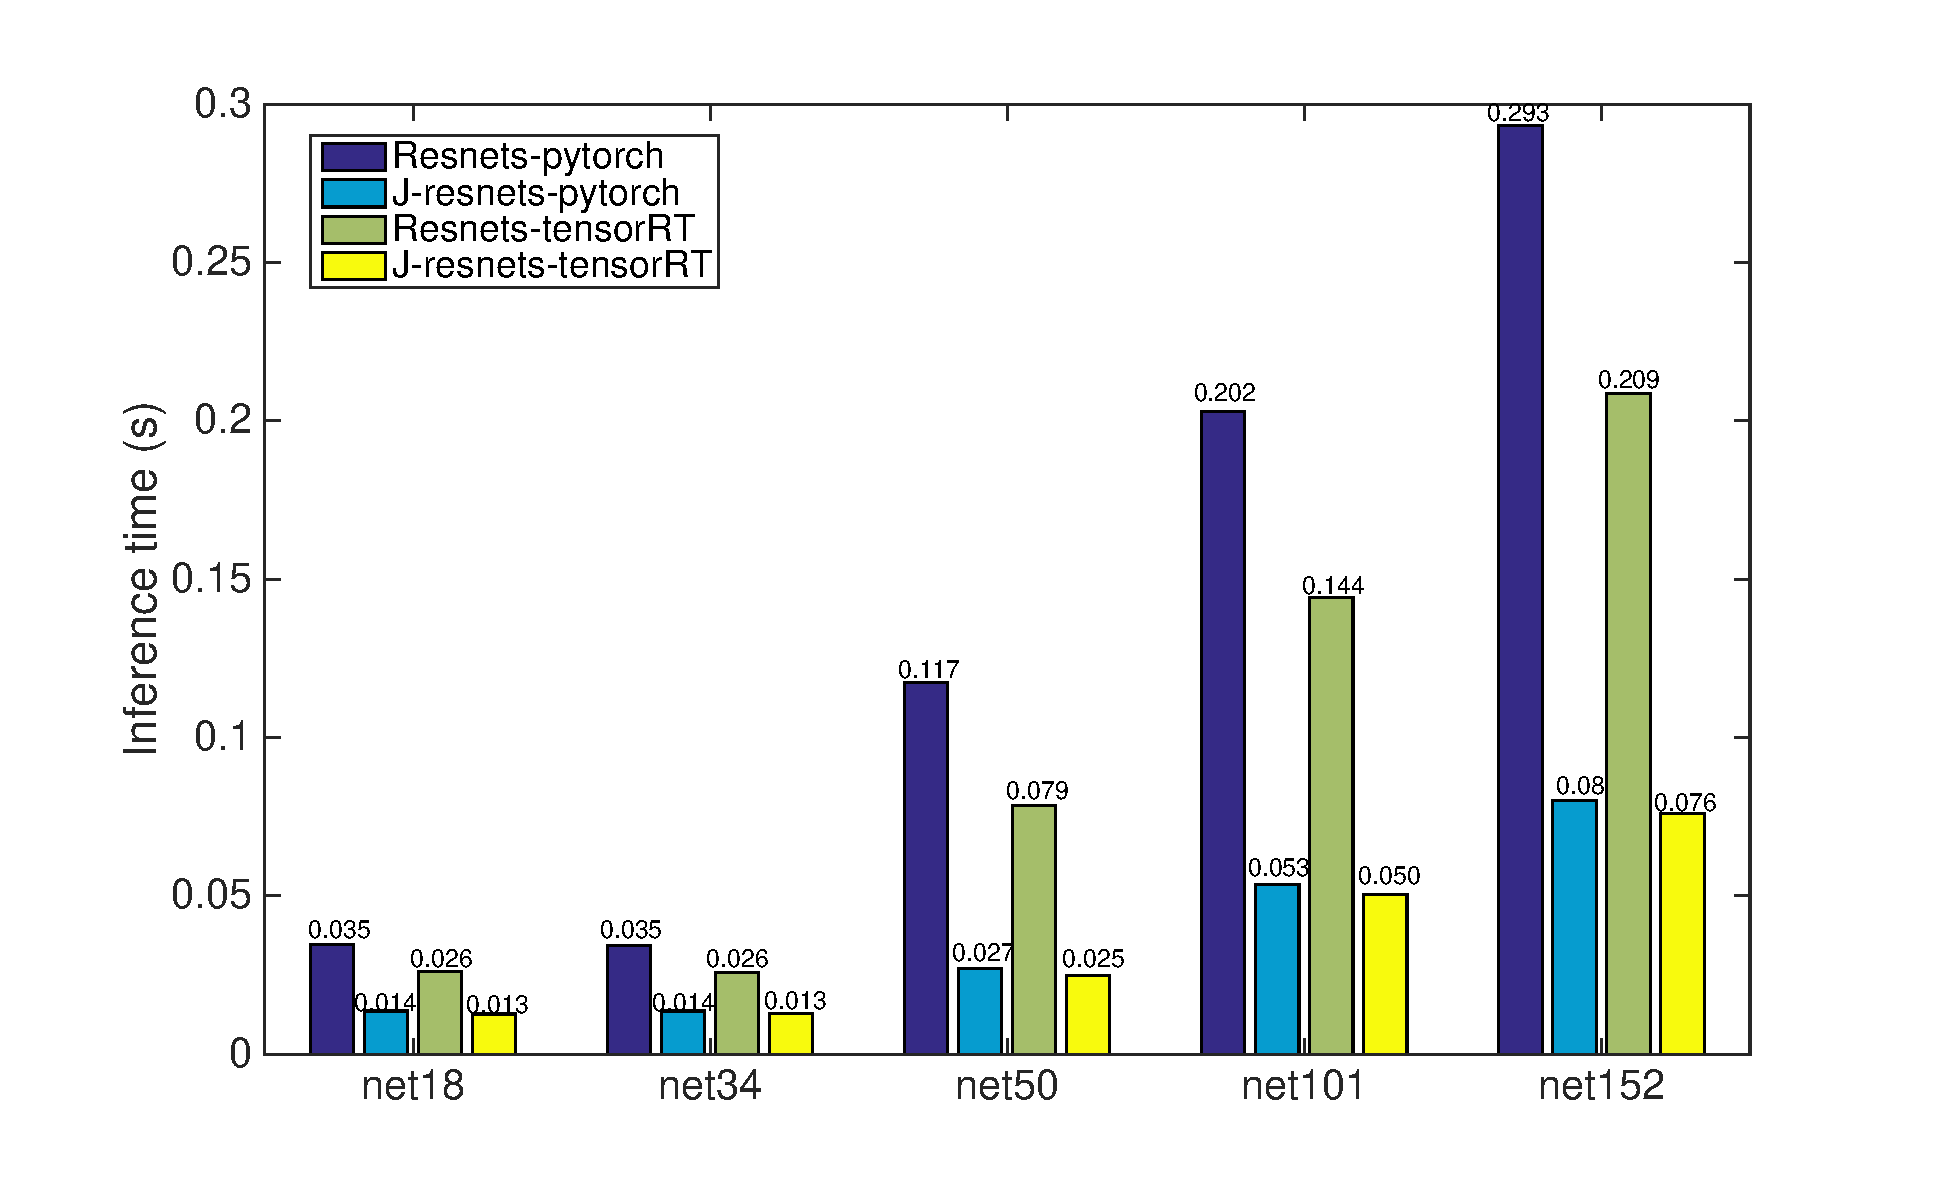
\includegraphics[width=1\textwidth]{figures/Jresnet/FIG8(a)_TII-21-2603.eps}
		\label{fig_first_case}}
	
	\subfigure[在NVIDIA Tx2上的实验结果]{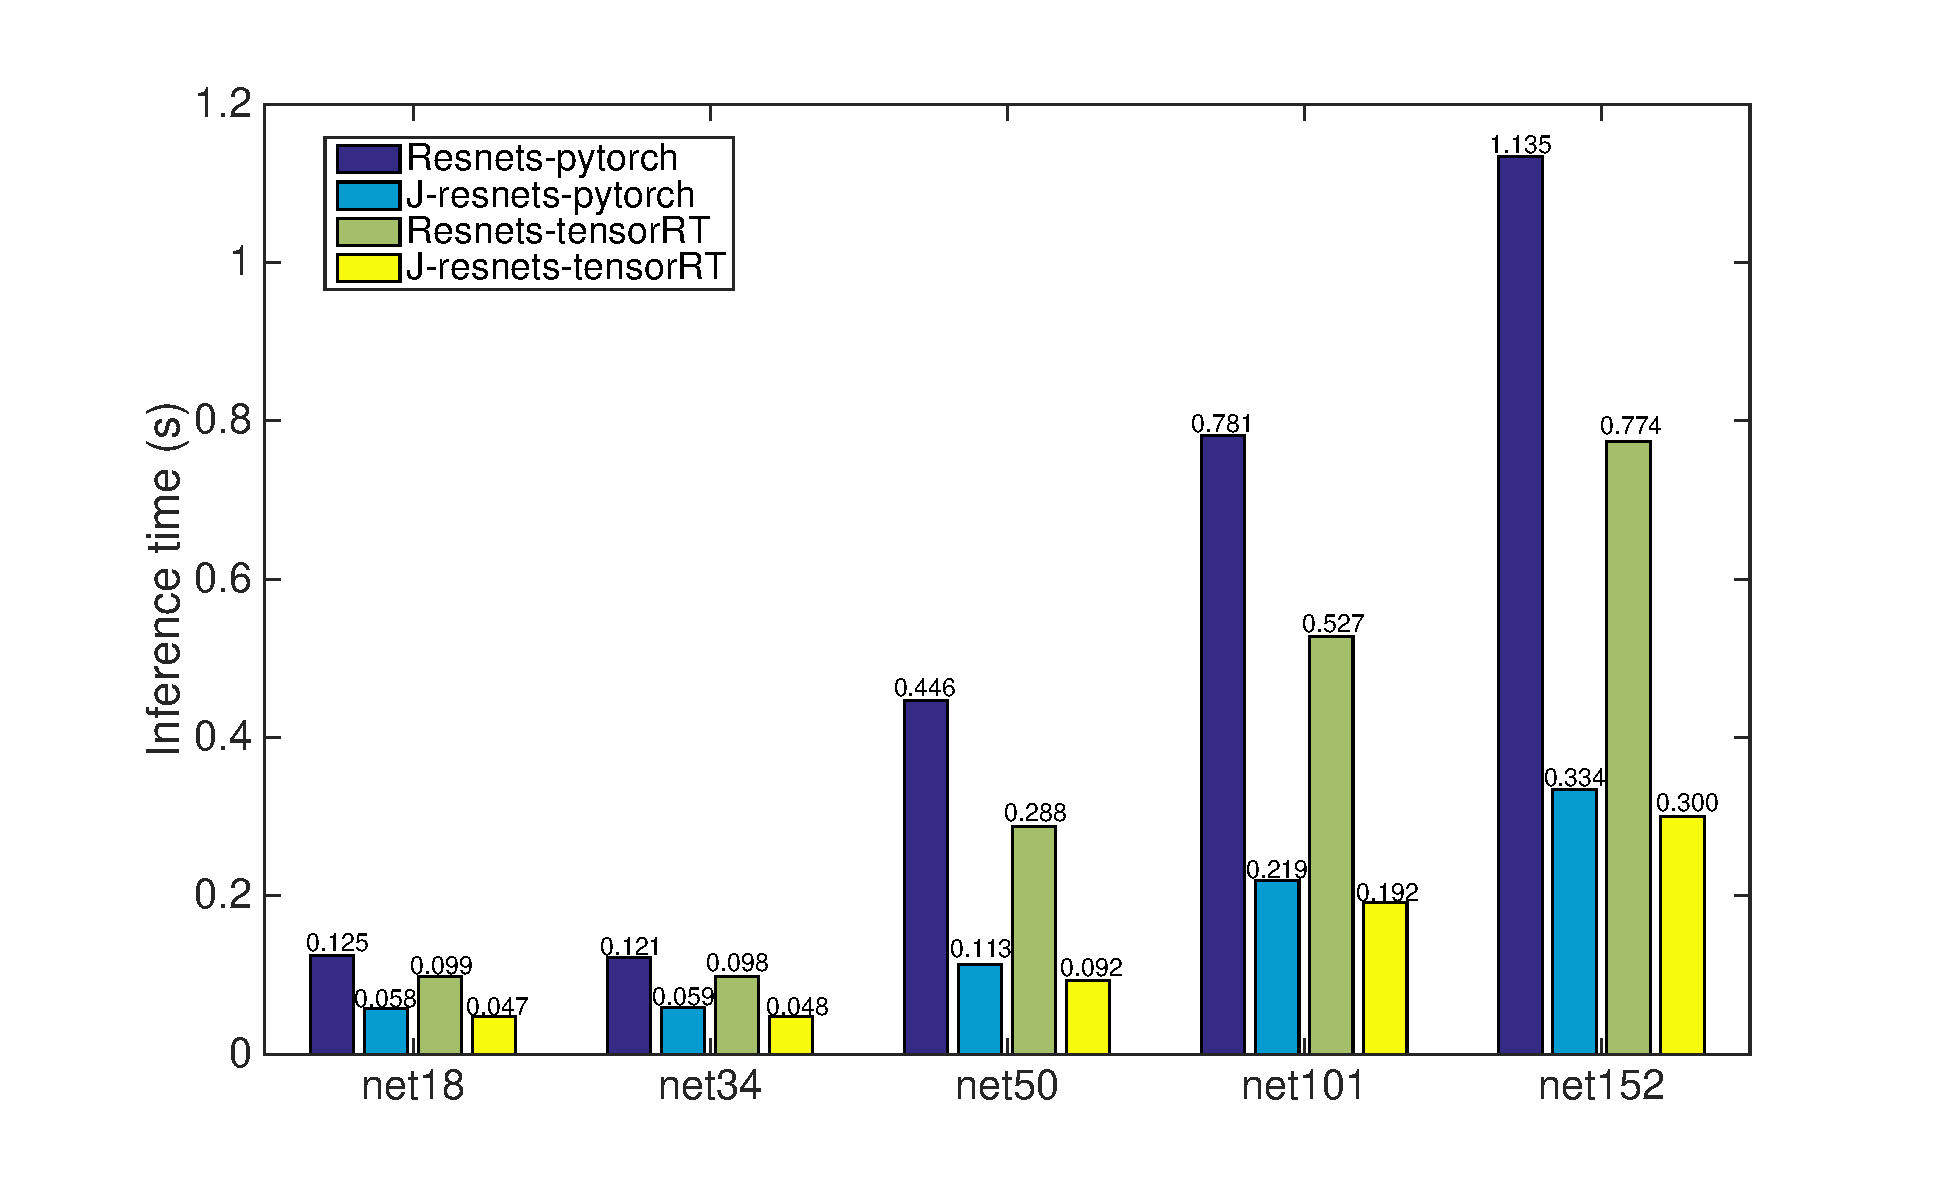
\includegraphics[width=1\textwidth]{figures/Jresnet/FIG8(b)_TII-21-2603.eps}
		\label{fig_second_case}}
	\caption{不同推理计算框架和不同硬件平台下\emph{Juggler ResNet}和\emph{ResNet}的推理性能比较。在预热硬件后,使用3通道256分辨率的输入图像,平均运行100次的实验结果。在Tx2上的参数设置batchsize = 1,在NVIDIA V100 GPU上的参数设置batchsize = 8。}
	\label{speed}
\end{figure*}


图\ref{speed}(a),(b)显示与原始\emph{ResNet}相比,Juggler-ResNet在NVIDIA Tx2上可实现3.95倍的加速,在NVIDIA V100上可实现4.31倍的加速。 这些结果表明,Juggler ResNet的加速效果不仅适用于硬件资源有限的平台,而且也适用于硬件资源丰富的平台。值得注意的是,加速效果随着网络深度的增加而增加。因为网络越深,内存访问、内核系统调用和上下文切换开销就越高。因此,与原始\emph{resnets}相比,线性拓扑结构的简单数据流在深度网络中的优势变得更加明显。

此外,Juggler ResNet在不同的推理计算框架上都实现了不同程度的加速效果,如图.\ref{speed}(a),(b)所示。 在不同的硬件条件下,它在\emph{Pytorh}框架上的加速最为显著,比原来的\emph{resnet}快2.05-4.31倍。即使在主流的推理加速框架TensorRT上,Juggler-ResNet的性能也比原始的\emph{resnets}高出3.17倍。值得注意的是,对比Juggler ResNet对Pytork和Tensorrt框架的加速效果,Tensorrt仅比Pytork快1.06-1.22倍,这与Pytork的推理速度几乎相同。因为所有推理计算框架在执行之前都会执行基于规则的图转换优化。这一结果表明,由于性能的提高实际上来自于它的线性拓扑结构,所以Juggler-ResNet的优化空间很少。 

\subsubsection{Throughput}

鉴于resnet152的参数量最多,这既可以显示优化性能的极限和硬件计算能力的拐点。因此,我们选择它作为比较模型。如图.\ref{throughput}所示,随着batchsize大小的增加,两个网络的曲线具有几乎相同的上升趋势。然而,Juggler-ResNet152在较大batchsize的大小设置下上的吞吐量明显优于ResNet152。在Tx2上,Juggler-ResNet152的峰值吞吐量是ResNet152的1.38倍。这种差距在V100上更为明显,V100上的Juggler-ResNet152的峰值吞吐量是ResNet152的3.22倍。

在图\ref{throughput}中,可以观察到Juggler-ResNet152能够在不同的硬件平台上快速达到峰值吞吐量。例如,在V100上,具有线性拓扑结构的Juggler-ResNet152分别在$batchsize=10$和$batchsize=36$时达到V100和Tx2硬件平台的峰值吞吐量。然而,多分支resnet152在$batchsize=64$和$batchsize=48$时达到峰值吞吐量。此外,我们观察到,当$bathsize=2^n+2$时,resnet152的吞吐量会显著出现一个下降。例如,在Tx2上,$bathsize=18$对比$bathsize=16$的吞吐量减少9.93\%,在V100上,$bathsize=18$对比$bathsize=16$的吞吐量减少6.51\%。这使得图中resnet152的吞吐量曲线呈现出明显的锯齿状上升趋势。然而,在$bathsize=2^n+2$设置下,Juggler-ResNet152的总体曲线更平滑,吞吐量没有明显下降。因此,当batchsize增加时,Juggler-ResNet152比ResNet152更快地达到最佳吞吐量,并且增长更稳定。

\begin{figure*}[t]
	\centering
	\subfigure[在NVIDIA V100上的吞吐量]{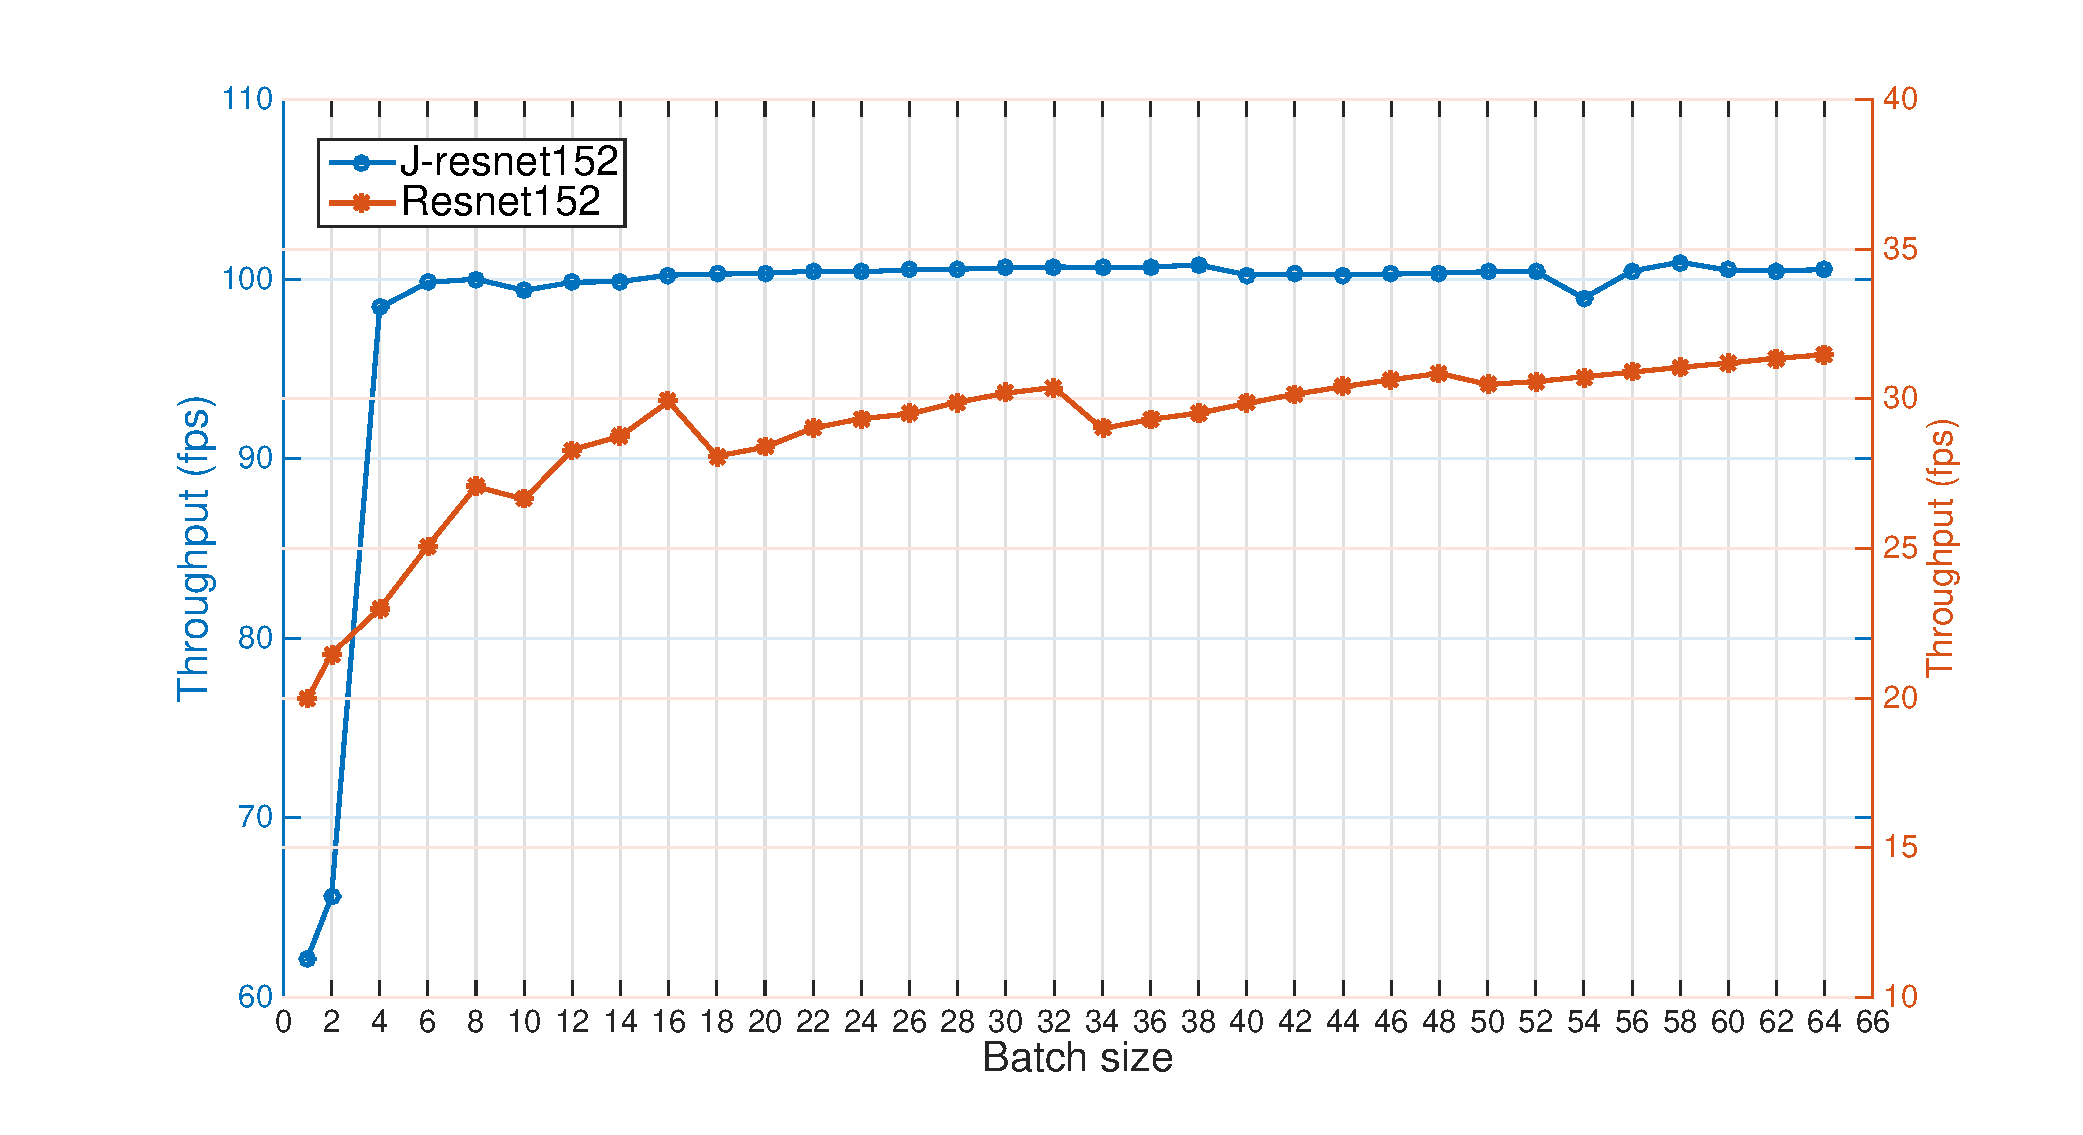
\includegraphics[width=1\textwidth]{figures/Jresnet/FIG9(a)_TII-21-2603.eps}
		\label{first_case}}
	\subfigure[在NVIDIA Tx2上的吞吐量]{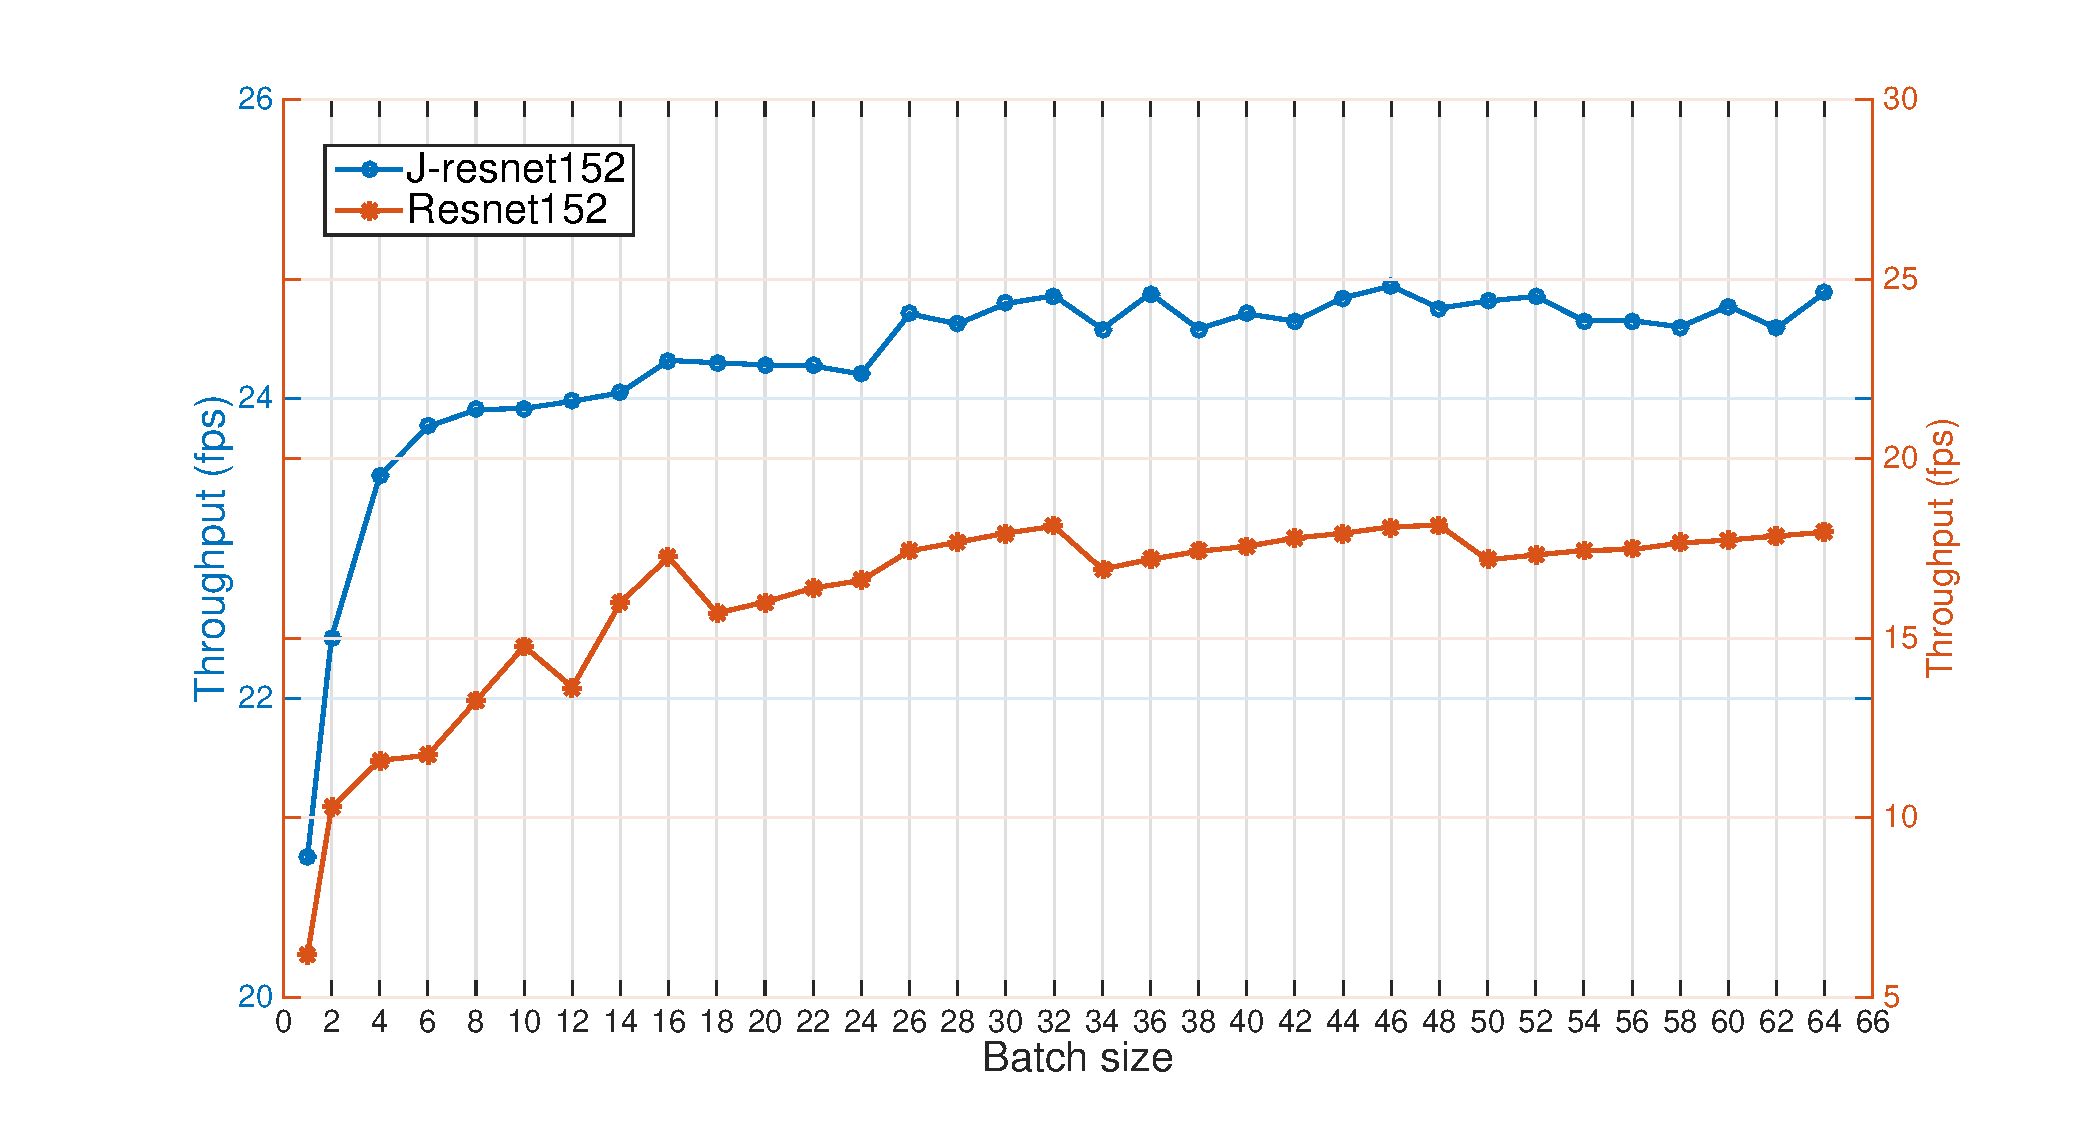
\includegraphics[width=1\textwidth]{figures/Jresnet/FIG9(b)_TII-21-2603.eps}
		\label{second_case}}
	\caption{在不同的批大小设置下,不同硬件平台上的Juggler-ResNet152和ResNet152的吞吐量。在预热硬件后,平均运行100次的实验结果。在Tx2上的输入图像是3通道56分辨率, 在V100上的输入图像是3通道256分辨率。}
	\label{throughput}
\end{figure*}

\begin{figure}[h]
	\centering
	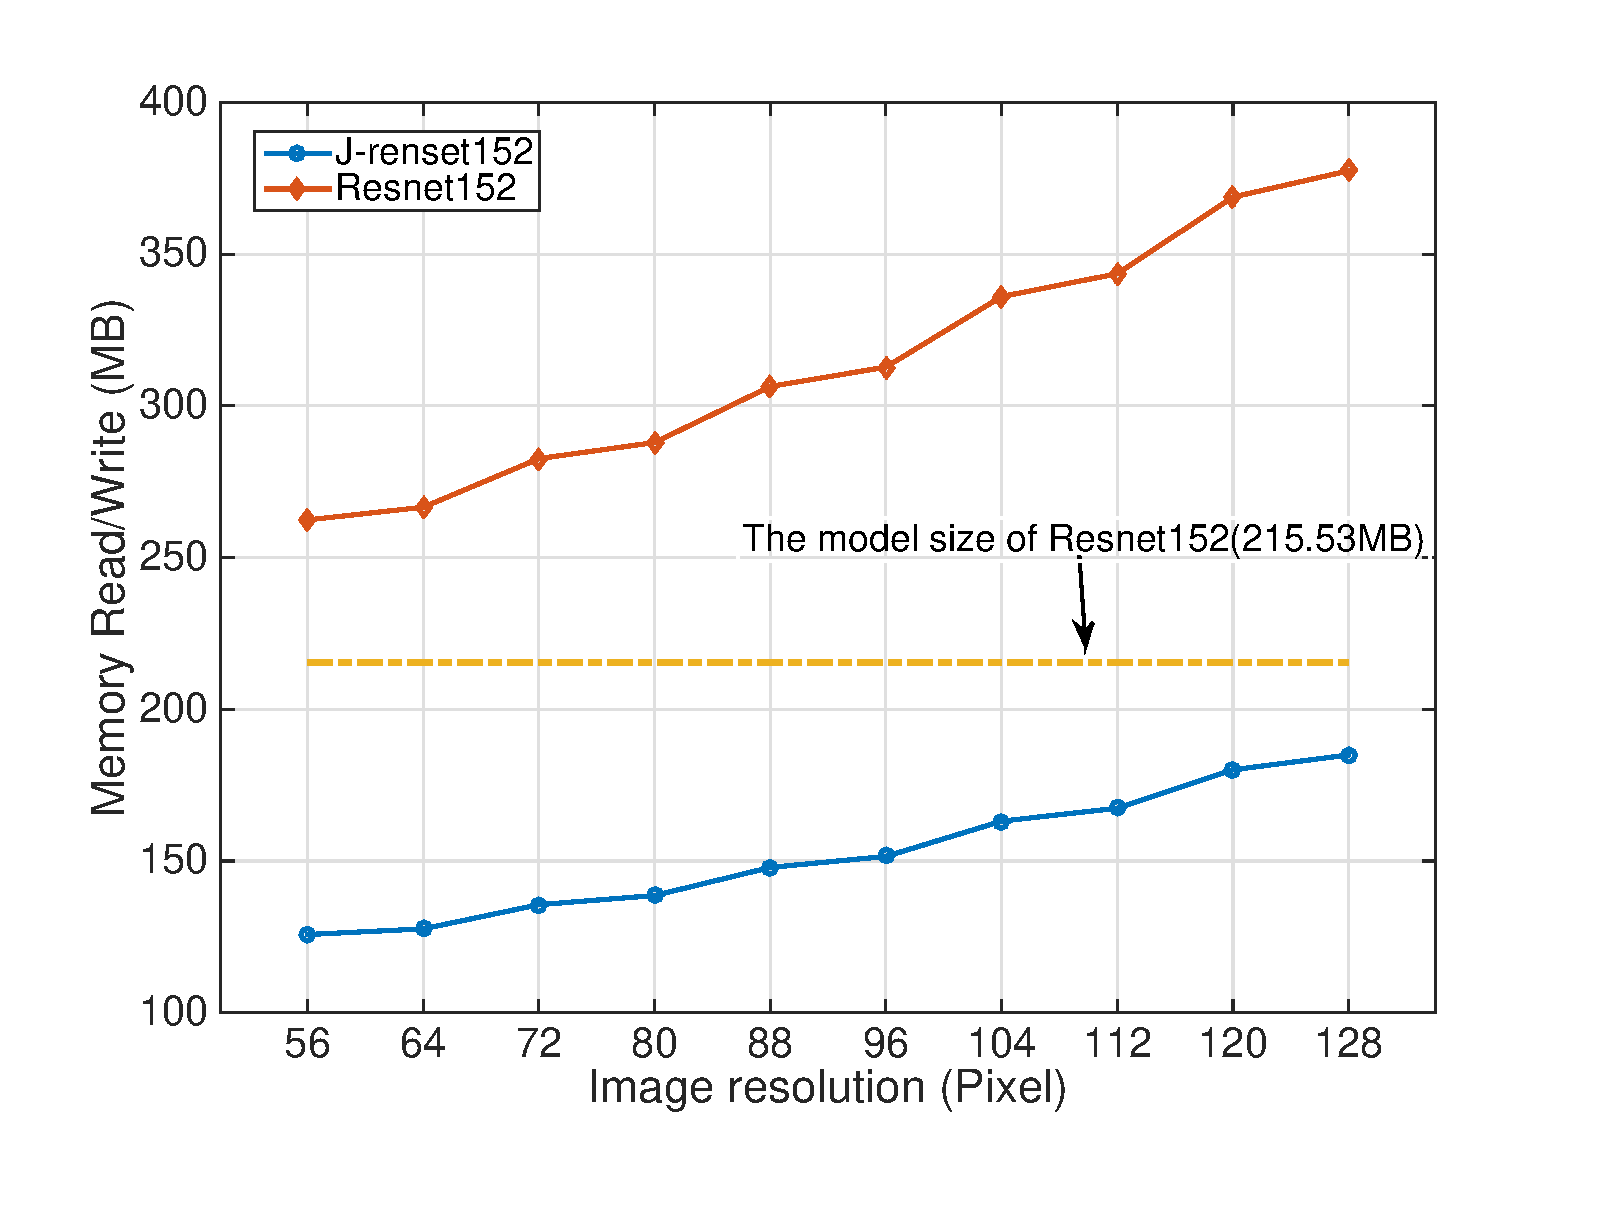
\includegraphics[width=1\textwidth]{figures/mem_WR.eps}
	\caption{内存读写量。}
	\label{memWR}
\end{figure}


%
%	\begin{algorithm}[H]
%		\caption{Convert Juggler-ResNet into liner-topology architecture}
%		\label{alm}
%		\begin{algorithmic} 
%			\Require A multi-branch architecture Juggler-ResNet $G_0$, a list of fusible residual structure $\{g_{1},g_{2},g_{3}......g_{n}\}$ of Juggler-ResNet and each $ g_{i}$ has convolution kernels layers $L =$ $\{conv_{1},conv_{2},conv_{3},sconv_{4}\}$, three fusion operator $F_{batch}(.)$ in \ref{sub1}, $F_{conv}(.)$ in \ref{sub2} and $F_{expand}(.)$ in \ref{sub3}.
%			\Ensure Liner-topology architecture Juggler-ResNet $G_1$.
%			
%			\State // $sconv_{4}$ represent the convolution kernel on the shortcut // connection in a fusible residual structure $ g_{i}$ with downsampling. 
%			\For{$i=1,\cdots,n$}
%			\State $g_i = F_{batch}(g_i)$
%			\State $Conv_{m} = F_{conv}(g_i.conv_{1},g_i.conv_{2})$
%			\State $Conv_{m} = F_{conv}(Conv_{m},g_i.conv_{3})$
%			\If{$g_i.sconv4 \neq \emptyset$}
%			\State $Conv_{e} = F_{expand}(g_i.sconv4)$
%			\State $Conv_{m} = Conv_{m}+Conv_{e}$
%			\EndIf
%			\State $g_i.L =Conv_{m}$
%			\EndFor
%			\State \Return $G_1$
%		\end{algorithmic}
%	\end{algorithm}
%

%\section{动态网络}
%
%深度神经网络已经广泛应用在计算机视觉、自然语言处理等领域,并且取得了较大的成功。近年来,越来越强大、越来越高效的神经网络模型设计(如 AlexNet[1] , VGG[2] , GoogleNet[3] , ResNet[4] , DenseNet[5] 以及 SENet[] 等)层出不穷,而近几年开始发展的NAS网络架构搜索技术[7],[8] 也在不断寻找强大高效的网络结构。然而,大多数当前流行的深度网络是静态的,具有相同的静态推理范式:一旦模型完成训练,网络的结构和参数在测试阶段都始终保持不变,这一定程度上限制了网络模型的表征能力、推理效率和可解释性[9],[10],[11],[12] 。
%
%如前所述,动态网络则可以在推理阶段根据输入样本的不同,自适应地调节自身的结构或参数,从而拥有诸多静态网络无法享有的良好特性。动态网络的优势有:
%
%\begin{itemize}
%    \item [1)] 
%    推理效率:很多动态网络可以通过选择性地激活模型中的模块(如网络层[10] ,卷积通道[13] 或子网络[14])来实现计算资源的按需分配,从而在更容易识别的样本上或信息量更少的区域位置(时间或空间)上节约冗余计算,提升推理效率。
%    \item [2)]
%    表达能力:通过动态地调节网络的结构或参数,网络模型可以拥有更大的参数空间以及更强的表达能力。例如,通过基于特征的动态集成多组卷积层权重[11],[15] ,可以在只增加极小计算开销的前提下显著提升模型参数容量。同时,动态网络可以集成常用的注意力机制,动态的评估因为输入的不同,根据不同通道[16] 、空间区域[17] 和时间位置[18]在推理阶段不同响应,对参数进行动态地重新加权。
%    \item [3)]
%    自适应性:相较于静态网络的固定计算量,动态网络可以在不同环境下,如不同的硬件平台,实现模型精度与效率的动态平衡。
%    \item [4)]
%    兼容性:动态网络并非“另起炉灶”,而是正交于现有的模型优化方案,可以与现有模型优化的其他先进技术相兼容,从而可以借助这些先进技术达到SOTA(技术发展水平,state of the art)性能。动态网络可以直接基于现有轻量化模型进行构建[19],也可以利用 NAS 技术[7],[8]。另外,动态网络也可以利用模型剪枝技术[20] 和模型量化技术[21] 等)进一步提升运算效率。
%    \item 通用性:动态网络已经被应用于多任务中,其中有图像分类[10],[22]、目标检测[23]、语义分割[24]等。另外,许多视觉任务中发展起来的技术可以被拓展至 NLP领域[25],[26],反之亦然。
%    \item 可解释性:利用动态网络,人们可以分析在处理一个样本时,网络激活了哪些模块[22],也可以分析输入中的哪些部分对最终的预测起决定性作用[29]。有研究指出了大脑处理信息的动态机制[27],[28],未来关于动态网络的研究可能会帮助人们更好的探索深度网络模型和大脑的内在的运行机制之间。
%\end{itemize}

%\section{卷积层通道激活特性的分析}
%
%以前关于通道减枝的研究[],根据评估卷积核通道显著性来对通道进行修剪,并从不重要的通道中删除所有输入和输出连接从而生成更小的密集模型。说明了通道对于不同数据的响应各不相同,其显著性不是静态的,而是和输入数据有一定的关系。基于此,我们对卷积层通道激活特性进行分析,力图发现相关规律。
%
%然而,基于显著性的剪枝方法有三个缺点。首先,通过删除频道,CNN的能力将永久丧失,而对于被删除频道负责的困难输入,由此产生的CNN可能永远无法恢复其准确性。其次,尽管信道剪剪可能会大幅缩小模型尺寸,但如果没有精心的设计,在一个CNN中不能有效地减少计算资源而不损害其准确性。最后,神经元的显著性不是静态的,这可以通过图1的特征可视化来说明。这里,CNN显示一组输入图像,卷积输出中的某些通道神经元可能会非常兴奋,而另一组图像从相同的通道中却几乎没有反应。
%
%\begin{figure}[]
%    \centering
%    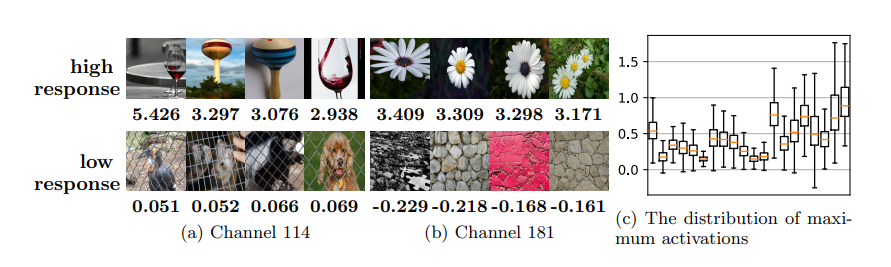
\includegraphics[width=0.9\textwidth]{subnet/active.png}	%\vspace{-1.0em}
%    \caption{ResNet18模型在ImageNet图片上部分卷积核的通道响应情况[]}
%    \label{fig:active} %\vspace{-0.8em}
%\end{figure}
%
%图~\ref{fig:active}为预训练的ResNet18模型在ImageNet验证数据集上的通道响应输出情况,其中(a)和(b)中最上面的一行分别对3b/conv2层块的114和181通道响应情况,(c)显示了前20个通道中观察到的最大激活的分布,每个图像下面的数字表示在通道添加快捷方式和激活前观察到的最大值。如图所示,卷积核之间的通道数相应输出出现了很大差异,某些通道的神经元可能会非常兴奋,而另一组图像从相同的通道中却几乎没有反应。
%
%\begin{figure}[]
%    \centering
%    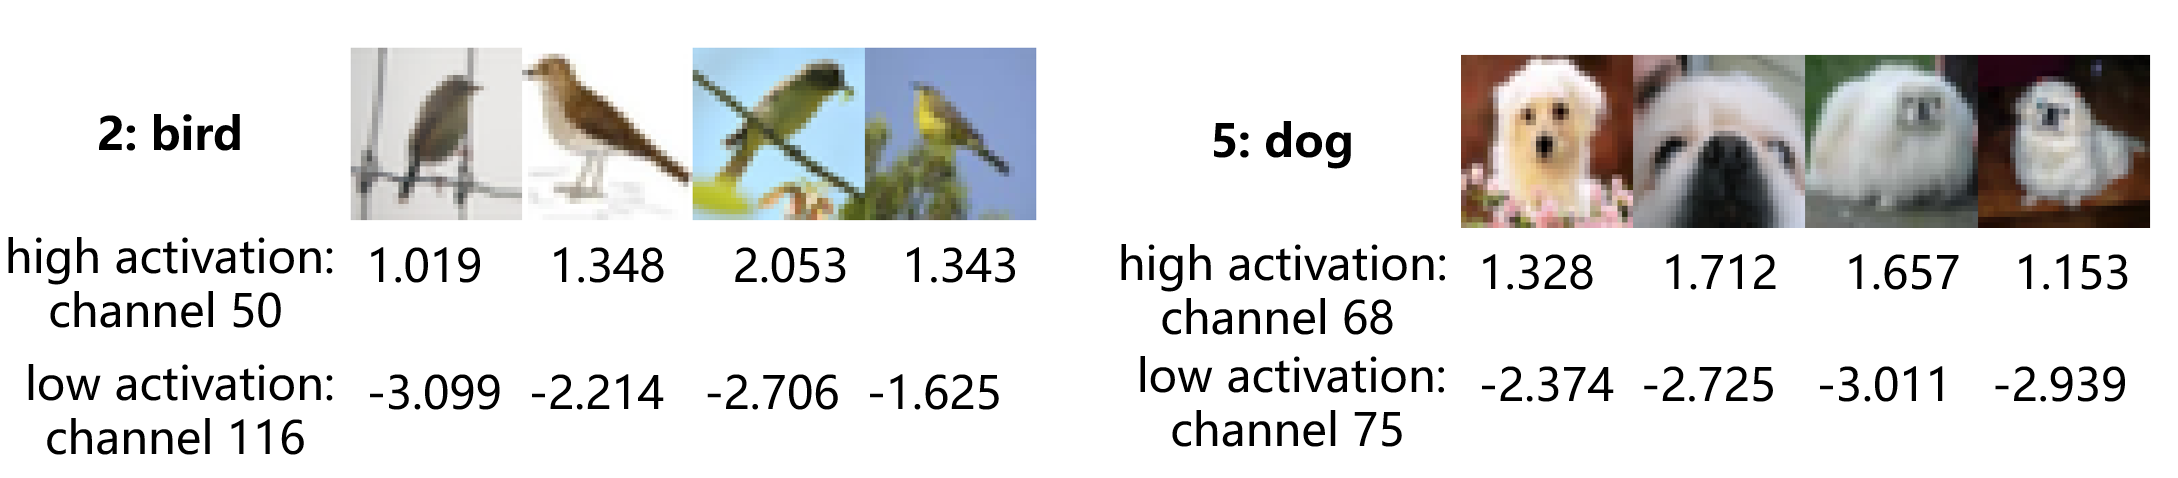
\includegraphics[width=0.9\textwidth]{subnet/channel-activation.png}	%\vspace{-1.0em}
%    \caption{ResNet18模型在CIFAR-10图片上部分卷积核的通道响应情况}
%    \label{fig:channel-activation} %\vspace{-0.8em}
%\end{figure}
%
%如图~\ref{fig:channel-activation}所示,在ResNet-18预训练模型的基础上,我们对CIFAR-10的每个图像类别进行不同模型层的激活强度评估。在CIFAR-10中,我们发现层块2a/conv2的输出在不同的图像类上差异很大,而在相似的图像上输出更一致。如图1所示。例如,鸟类的图像极大地激活了第50通道的神经元,而在第116通道却很少引起激活,而狗的图像在第68通道的激活程度很高,在第75通道的激活程度较低。
%
%\section{任务感知的子网络划分}
%
%我们发现相似的图像具有相似的通道显著性(见图~\ref{fig:channel-activation}),进一步的,我们将激活强度按通道的顺序排列成向量,使用向量 $\vec{v_c}$ 来表示 $c$ 类通道的显著性,其中 $a_{ij}$ 为 $c$ 类在第 $i$ 个卷积层和第 $j$ 个通道的平均激活值,$N$ 为卷积层数, $C_i$ 为第 $i$ 个卷积层。如此 $\vec{v_c}$ 表示如下:
%
%\begin{equation}
%    \vec{v_c} = [a_{00}, a_{01}, a_{02}, ... , a_{NC_{i-1}}, a_{NC_i}] \label{con:feature-vector}
%\end{equation}
%
%\begin{figure}[h]
%    \centering
%    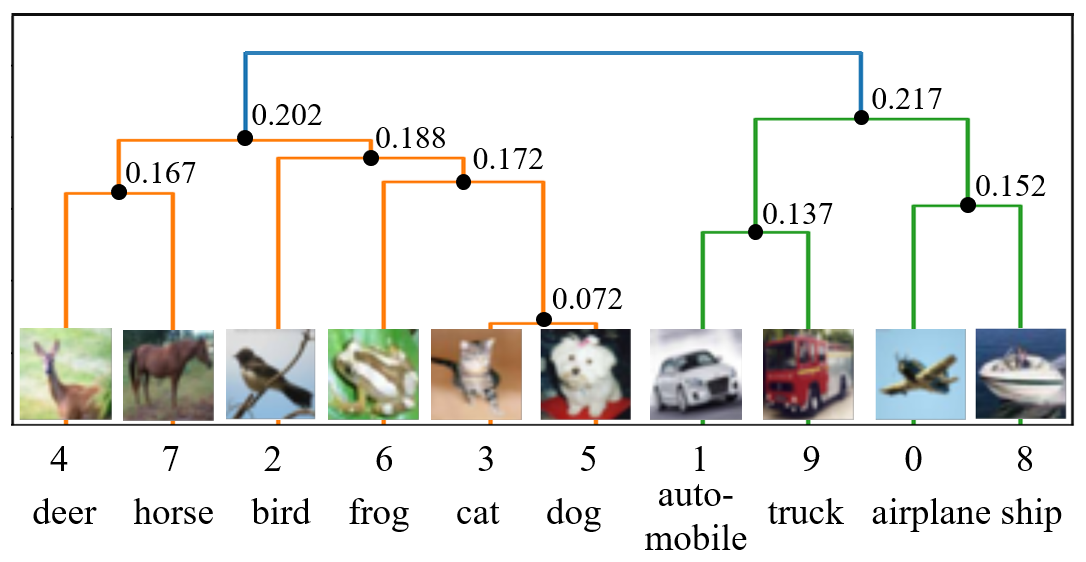
\includegraphics[width=0.9\textwidth]{subnet/cluster.png}	%\vspace{-1.0em} 
%    \caption{对CIFAR-10的10个图像类的聚类结果。结点上的数字表示两个分支之间的余弦距离,横轴表示它们的类数。}
%    \label{fig:cluster} %\vspace{-0.8em}
%\end{figure}
%
%为了探究通道激活和输入数据的特性,我们对不同类别的 $\vec{v_c}$ 进行聚类,在本文中,我们使用余弦距离来表示不同 $\vec{v_c}$ 之间的相似性距离,通过层次聚类来得到图像类之间的关系。图~\ref{fig:cluster}为ResNet-18网络和CIFAR-10数据集上的聚类结果。如图~\ref{fig:cluster}所示,第1、9、0、8类图像对于Resnet18模型的每一层都具有类似的激活强度。换句话说,ResNet-18认为这些图像类是非常相似的图像。因此,可以使用动态网络将根据聚类结果划分子网,同一个子网对这四个类进行后续的高维特征提取和分类。
%
%根据聚类结果,可将其划分为2个子任务。为了获得一个简单和有效的子网分类器,我们推荐更少的子任务划分。每个子网单独负责其对应的数据的推理工作,此时其他子网参数并不参与计算。如图~\ref{fig:subnet}所示,为子网络工作说明,根据输入类别从整个网络中推导出相应的子网,并动态选择关键子网进行推理,而不是使用整个网络。
%
%\begin{figure}[h]
%    \centering
%    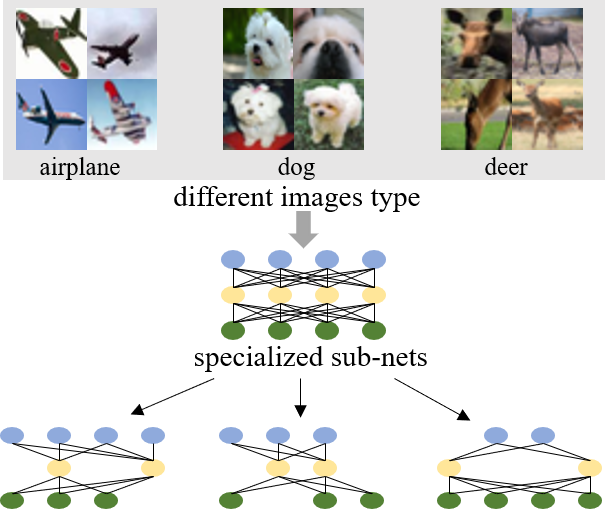
\includegraphics[width=0.8\textwidth]{subnet/sub-net.png}	
%    \caption{子网络和相应图像类的说明。根据输入类别从整个网络中推导出相应的子网,并动态选择关键子网进行推理,而不是使用整个网络。}
%    \label{fig:subnet}    %\vspace{-0.8em}
%\end{figure}
%
%\section{通道选择因子}
%
%子任务划分完成后,将创建子网络,子网络的参数由整个网络共享。由于通道激活值在不同任务类型之间的变化,在一定程度上它也显示了通道的重要性。因此,我们使用集合 $S=\{s_1, s_2, ... , s_n\}$ 描述了整个网络的连接方法,其中 $s$ 表示卷积层每个通道的选择因子,其反映了通道的重要性。然后对网络权值和选择因子进行训练,对选择因子进行稀疏正则化。训练后,我们直接将小于选择阈值的 $s$ 设为 $0$。之后,基于 $S$ 构建子网。在训练中,损失函数为:
%
%\begin{equation}
%    Loss_{new} = Loss_{origin} + \lambda \cdot \sum_{s \in S} ||s||_1
%\end{equation}
%
%其中 $Loss_{origin}$ 是一个CNN的正常训练损失,$|\cdot|_{L1}$ 是一个L1范数的稀疏选择因子,$\gamma$ 目的是平衡正则程度。
%
%\begin{figure}[h]
%    \centering
%    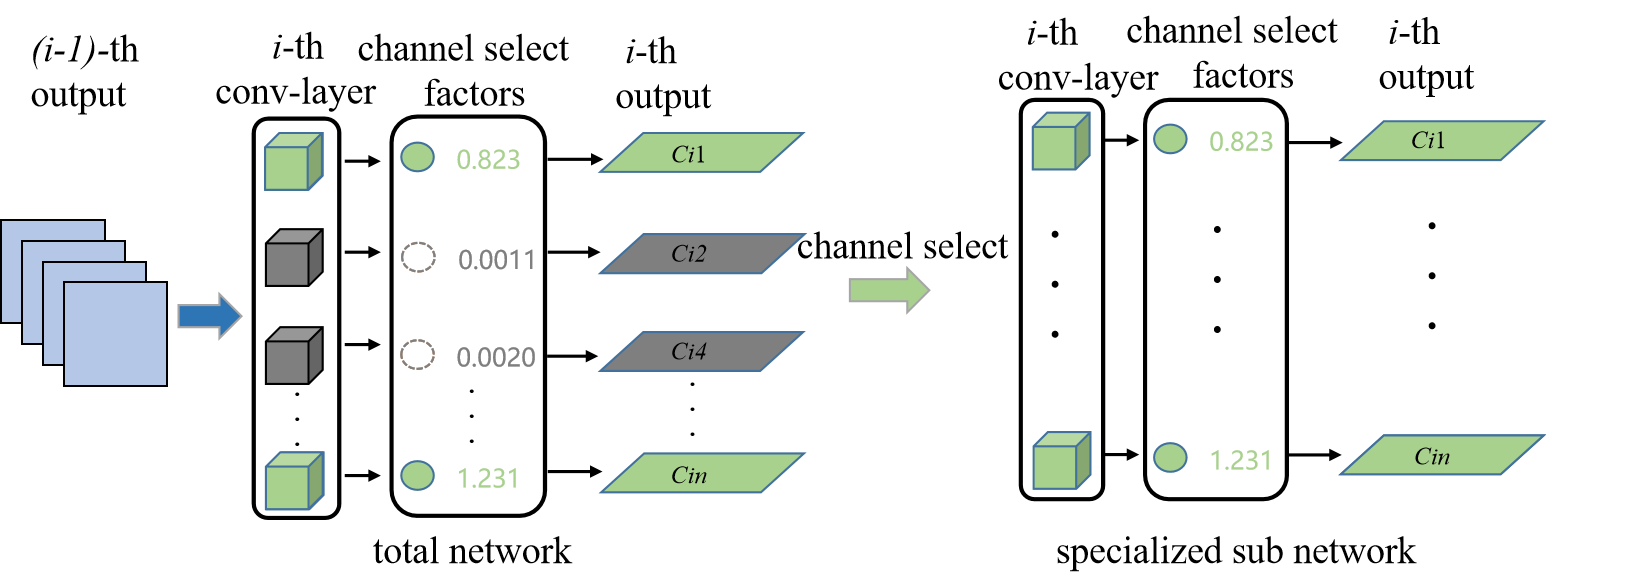
\includegraphics[width=0.9\textwidth]{subnet/channel_select.png}
%    \caption{子网络划分过程}
%    \label{fig:channel-select} \vspace{-0.8em}
%\end{figure}
%
%如图4所示,在卷积层中,每个通道都有一个选择因子。通过在训练过程中对这些因子进行稀疏正则化,以此训练其可以自动识别不重要的通道。再训练中,通过将小选择因子设置为0,我们获得了一个专门的子网(右侧),然后对其进行微调,以达到与整个网络相当的精度。将小的选择因子设置为0,我们就可以得到一个合适的子网。
%
%在这个过程中,对于每个子网,只添加非常少量的参数用以表示其信道选择,如图~\ref{fig:subnet-select}。在部署时,对于非零选择因子,在子网加载时纳入批数层。我们知道批归一化从层(BN层)的计算公式为:
%
%\begin{equation}
%    z_{out} = \gamma \cdot \frac{z_{in} - \mu_B}{\sqrt{\sigma^2_B + \epsilon}} + \beta
%\end{equation}
%
%我们使用 $\gamma^{'}$ and $\beta^{'}$ 替换上式中的 $\gamma$ and $\beta$:
%
%\begin{equation}
%    \gamma^{'} = s \cdot \gamma ; \beta^{'} = s \cdot \beta
%\end{equation}
%
%\section{关键子网络激活}
%
%通过任务感知的动态子网络,能够根据输出动态的跳过无关的参数计算,从而加快整个网络的推理速度,但是这并不能降低网络的运行时内存需求,甚至因为要存储额外的参数和额外的子网分类器,还会增加少许内存占用。在此,我们提出了一个关键的子网激活方案来减少内存消耗,并协助推理框架更好地做出交换决策。在本研究中,关键子网是指当前运行的推理任务中不可缺少的子网。该方案能够准确地获取关键子网的数据而不是不相关子网。
%
%\begin{figure}[h]
%    \centering
%    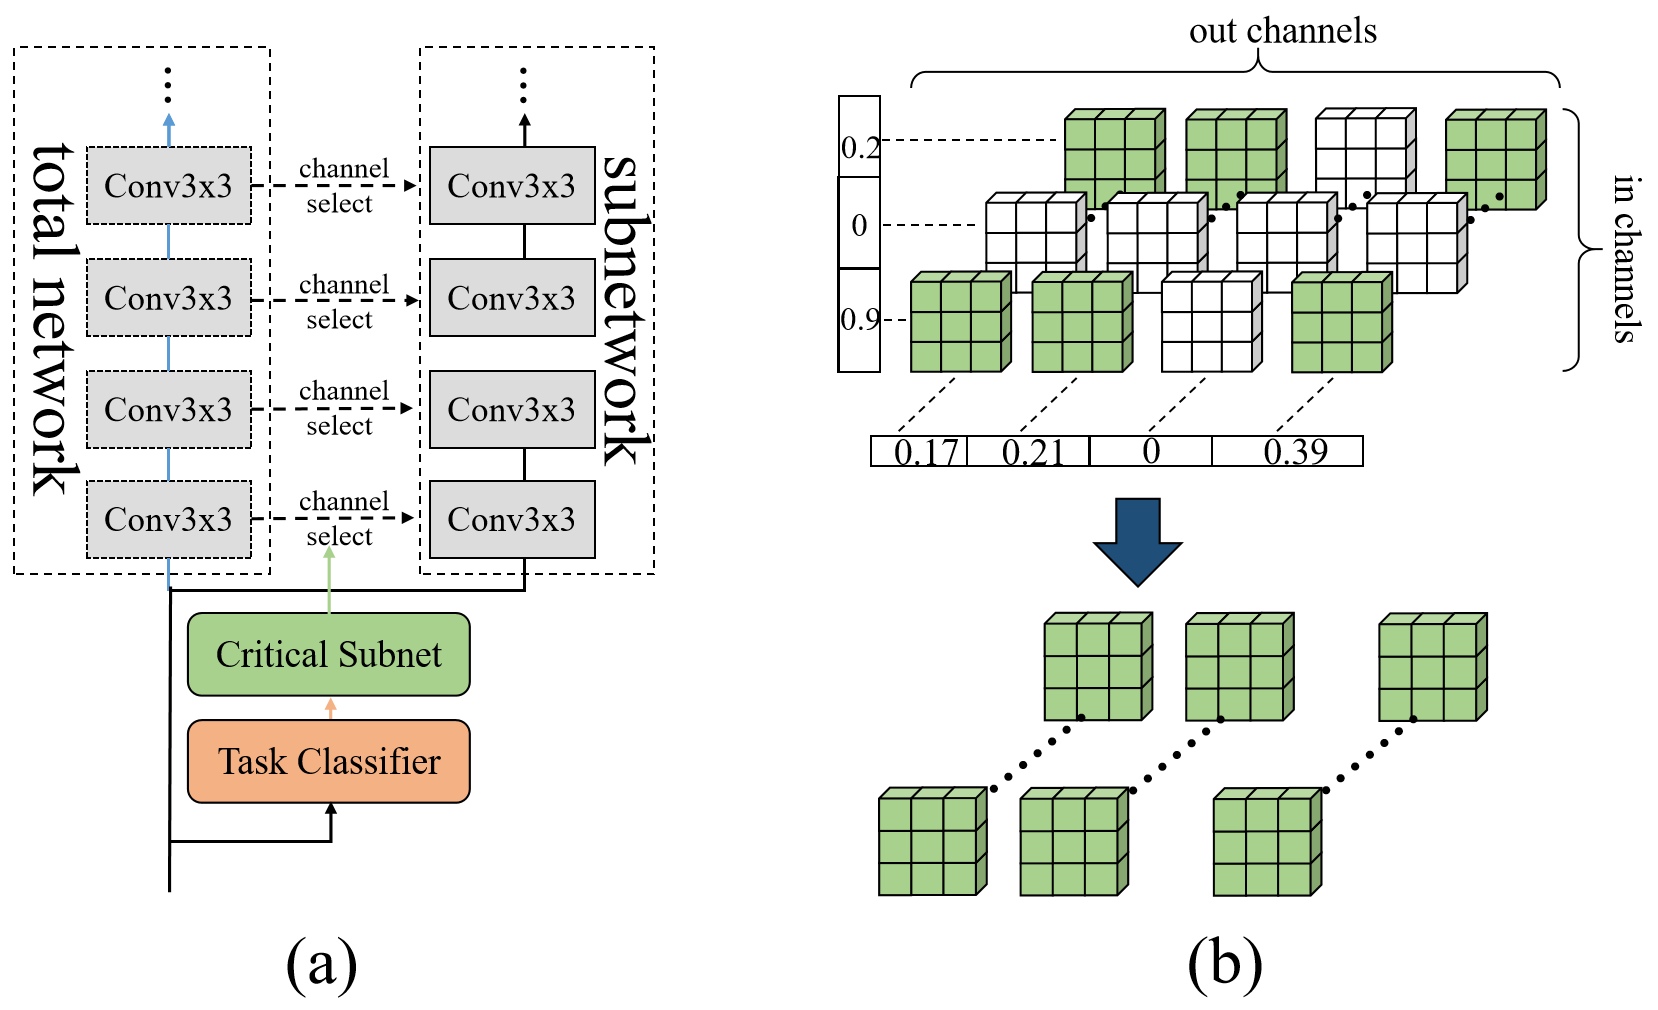
\includegraphics[width=0.9\textwidth]{subnet/subnet_activation.png}	
%    \caption{(a) 表示快速图像类识别的任务分类器。它共享整个网络的前两层,识别输入的任务类型,然后通过信道选择因子激活关键子网。(b)利用通道选择因子选择性加载关键子网参数的方法。}
%    \label{fig:subnet-activation} 
%\end{figure}
%
%\begin{figure}[h]
%    \centering
%    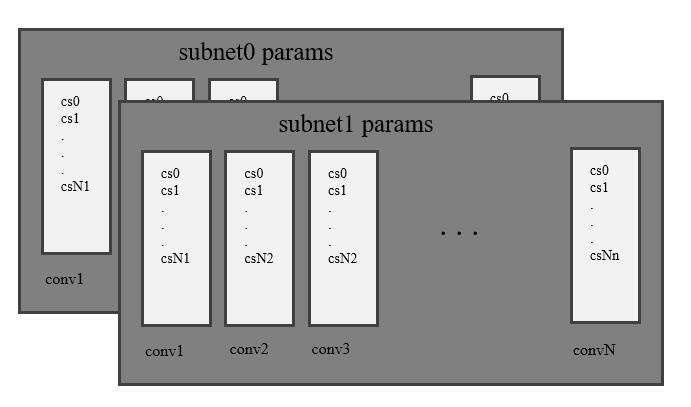
\includegraphics[width=0.9\textwidth]{subnet/subnet.jpg}
%    \caption{子网络选择因子}
%    \label{fig:subnet-select} \vspace{-0.8em}
%\end{figure}
%
%由于每一组子网有效地工作于特定的任务类型,我们需要在子网激活前预测进入图像的类别。如图\ref{fig:subnet-activation}(a)所示,在推理开始使用快速任务分类器,利用之前计算的卷积结果为推理任务选择相应的子网。其中选择子网络之后,需要根据子网络的选择因子参数(如图~\ref{fig:subnet-select})来激活相应的子网络参数,假设子任务是通过类的通道显著性特征聚类产生的(如公式\ref{con:feature-vector}所示),这些子任务的数量较少,因此只需要一个小规模网络就可以对子任务进行精确的分类。基于子网数量和分类要求,快速任务分类器可以简洁地进行分类,提高分类效率。
%
%图图\ref{fig:subnet-activation}(b)展示了子网络激活过程。在加载子网参数时,通过信道选择因子选择性地加载当前层的权值参数。这种修剪后的小尺度网络模型可以降低内存消耗和计算成本。注意,与以往的剪枝研究不同,我们没有抛弃任何网络或参数;相反,关键子网的必要参数将被选择性地加载到当前任务中,而剩余的参数可以被激活到以后的任务中。
%
%\section{任务感知的子网络交换}
%
%\begin{figure}[h]
%    \centering
%    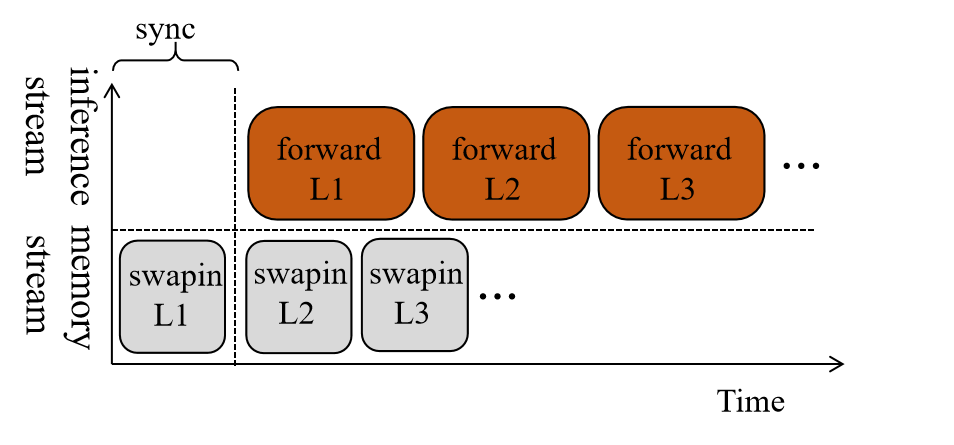
\includegraphics[width=0.9\textwidth]{subnet/swapin.png}
%    \caption{参数的交换方法的说明} \label{fig:swapping}
%    \end{figure}
%
%在此基础上,我们提出了一种新的任务感知交换(Task-Aware Swapping,TAS)算法,在推理框架层扩展内存空间。其基本思想是将未使用子网的冷数据交换到闪存中,并确保关键子网的数据在访问之前提前加载于内存之中。为了最小化权重参数加载延迟,我们使用pipeline进行参数加载和推力计算,不需要等待所有权重参数加载完成,在第一层加载完成后就可以开始进行推理。
%
%任务感知交换的工作过程如下。首先,传入的图像被缓冲在内存中。其次,基于快速任务分类器识别的图像类激活关键子网。读取已调优的子网有助于避免从无关子网中不必要地交换冗余数据。最后,将关键子网的数据,如参数和模型,预取到内存中。如图~\ref{fig:swapping}所示,为了提高交换效率,模型参数的交换操作可以通过正向推理的执行实现流水线化,从而隐藏I/O开销。正向推理时间通常大于交换时间。在本例中,数据同步(sync)后,第1层(L1)和第2层(L2)的正向推断时间可以与第2层(L2)和第3层(L3)的交换时间重叠。使用这种方法,几乎所有层(除了第一层)的交换时间都可以成功地与正向推理时间进行流水线化。这样,就可以将任务无关参数压缩在闪存中,从而节省了运行时内存。使用较大的顺序读取来获取这些数据,可以避免对数据碎片进行昂贵的块读取。注意,由于推理任务的模型和参数是只读的,它们在内存中永远不会变脏,所以交换只需要在推理过程中处理交换操作。
%
%\section{子网方案实现成本}
%
%为了实现关键子网络激活,引入了任务分类器在推理开始时快速识别图像类,从而产生额外的推理时间。根据不同图像的通道显著性相似度对子任务进行划分。由于嵌入式识别系统的图像类有限,简单的任务分类器只需要一个小规模的网络,这限制了时间开销。注意,在极端情况下,如果聚类结果甚至不在图像类之间(如手写数字图像),则不可能进一步划分网络。在这种情况下,只能导出一个子网,该子网将回归到传统的剪枝方法。
%
%\section{实验结果与分析}
%
%在本节中,我们在实际的算力较低的嵌入式设备TX2上进行了部署推理实验,将我们的TAS方法与传统减枝方法进行对比。其中,剪枝率为剪枝后的信道数与总信道数之比。
%
%\subsection{实验设置}
%
%在本次实验对比中,我们将所提出的任务感知交换(\textbf{TAS})与原始DNN模型和剪枝方法[20](\textbf{Prune})进行了比较。注意,TAS是在Prune的基础上实现的,并在此基础上集成了任务感知的子网交换策略。在实验中,我们使用NCNN[21]作为神经网络推理计算框架。在CIFAR-10数据集[8]上对DNN模型VGG16BN[22]进行训练和验证。
%
%\subsubsection{硬件平台说明}
%
%我们的实验基于Nvidia TX2嵌入式平台,搭载四核ARM®Cortex®-A57 MPCore, 8GB 256位LPDDR4内存,32GB eMMC flash存储设备,运行Ubuntu 18.04。其配置如表~\ref{tab:tx2}所示。
%
%\begin{table}[]
%    \centering
%    \caption{Nvidia TX2配置表}
%    \label{tab:tx2} %\vspace{-0.8em}
%    \begin{tabular}{|l|l|}
%    \hline
%    OS   & Ubuntu 18.04 bionic            \\ \hline
%    CPU  & HMP Dual Denver + Quad ARM A57 \\ \hline
%    GPU  & Nvidia Pascal 256 CUDA cores   \\ \hline
%    RAM  & 8GB 128-bit LPDDR4             \\ \hline
%    DISK & 32GB eMMC                      \\ \hline
%    \end{tabular}
%\end{table}
%
%\subsection{实验结果}
%
%本小节提出推论延迟,准确性和内存需求的结果。使用TAS将网络划分为两个子网(subnetwork0和subnetwork1),如上文分析。
%
%\begin{figure}[h]
%    \centering 
%    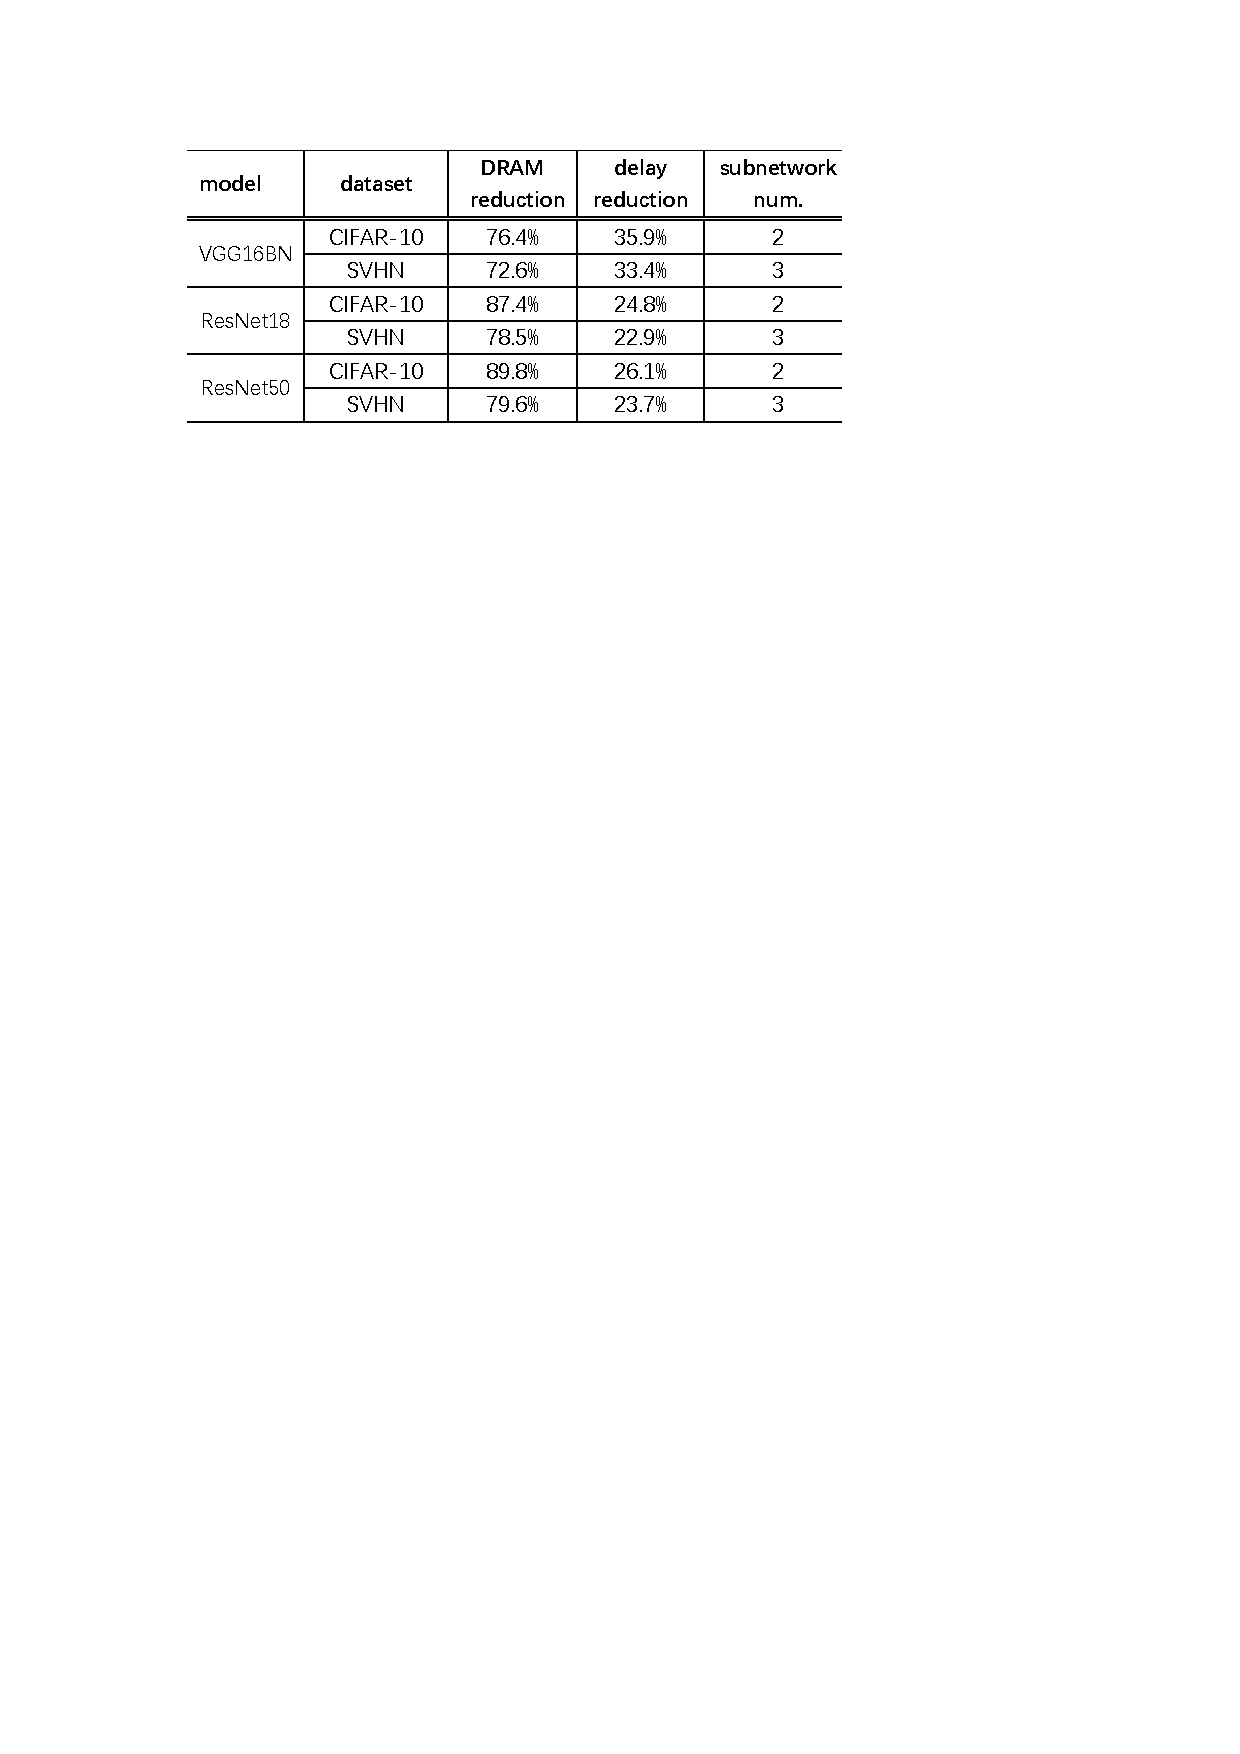
\includegraphics[width=0.8\textwidth]{subnet/more-models.pdf}	
%    \caption{不同模型和数据集的DRAM和推理延迟减少的结果。} \label{fig:more-models}
%\end{figure}
%    
%\begin{figure}[t!]
%      \centering
%     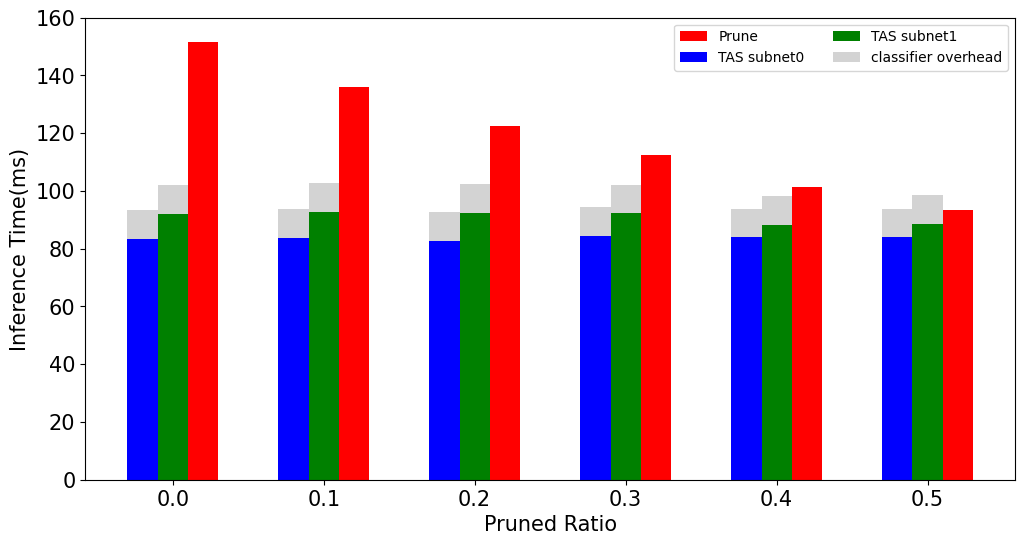
\includegraphics[width=0.8\textwidth]{subnet/timespeed.png}
%      \caption{分类器的时间开销和不同修剪程度下的总推理时间。}
%      \label{fig:classifier-result}
%\end{figure}
%
%\begin{figure}[h]
%    \centering
%     \subfigure[]{ 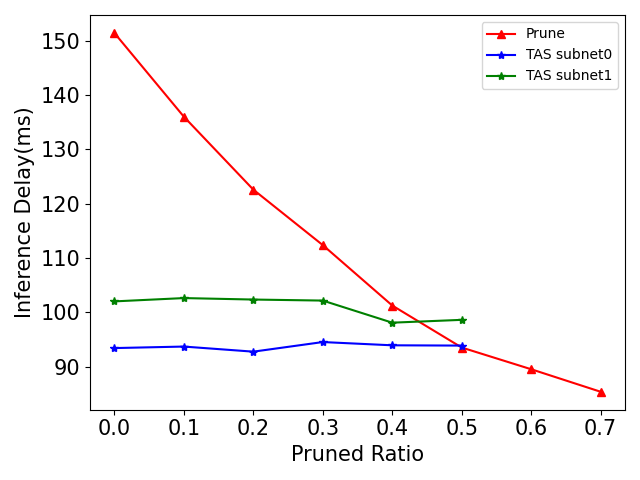
\includegraphics[width=0.6\textwidth]{subnet/runtime.png}}
%     \subfigure[]{ 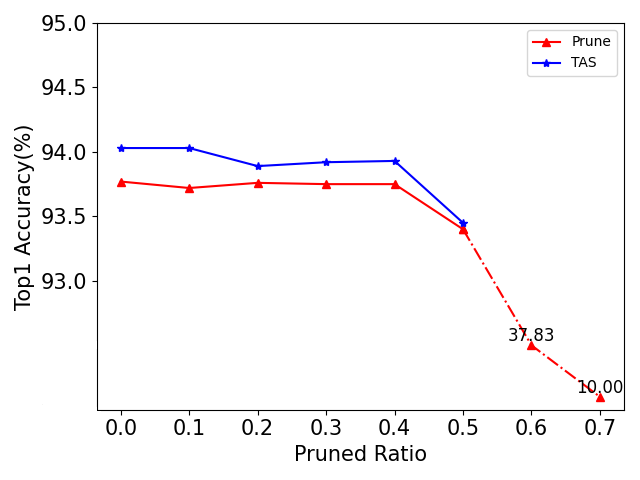
\includegraphics[width=0.6\textwidth]{subnet/top1acc.png}}
%     \subfigure[]{ 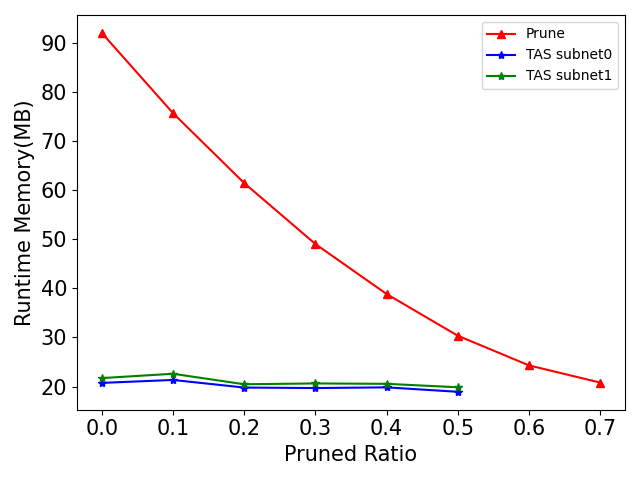
\includegraphics[width=0.6\textwidth]{subnet/runmem.png}}
%    \caption{(a)推理延迟(b)推理准确性(c)运行时内存消耗的结果。} 
%    \label{fig:result}
%\end{figure}
%
%
%
%\begin{itemize}
%    \item[1)] 性能与精度: 图~\ref{fig:result}(a)和(b)显示了推理延迟和准确性。使用传统的修剪方法(\textbf{Prune}), 当修剪比率为0.7时,产生的加速效果最高,相比原模型(修剪比例是0)推断延迟可以显著减少从151.5 $ms$ 到 85.4 $ms$。另一方面,与修剪比例大于0.6时,模型精度开始快速下降。这表明,过度修剪可能导致明显的精度下降。相比之下,提出的TAS方法在不同图像类别的性能和精度方面都优于\textbf{Prune}。\textbf{Prune}的精度甚至高于\textbf{Prune},因为划分的子网(subnetwork0和subnetwork1)具有更小的输入图像类和更少的通道,从而消除了无关卷积核产生的干扰噪声。因此,TAS进一步降低了网络复杂性,提高了推理精度。最重要的是,TAS保证了全模型结构的精度,同时减少了推理时间。另一方面,由于最小的子网数据读取量和流水线方案的高效率,交换开销只占总推理时间的0.3 \% 。由于层的深度通常比较大,例如VGG16BN模型有16层,所以第一层的加载时间对整体任务的影响有限。
%    \item[2)] 内存缩减: 图~\ref{fig:result}(c)显示了运行时内存消耗。对于TAS,它总是为subnetwork0和subnetwork1任务保持较低的内存消耗水平(大约20 MB)。例如,当整合到未修剪网络(修剪比为0)时,subnetwork0和subnetwork1任务对TAS的DRAM消耗分别为21.7 MB和20.7 MB,而未修剪网络的内存消耗则高达92.0 MB。这是因为TAS精确地按照实际推理要求激活了子网,避免了无关网络对内存的不必要使用。注意,当修剪率为0.5时,修剪达到了精度要求下的修剪极限。在这一点上,与Prune相比,TAS仍然实现了34.6\%的DRAM减少。图~\ref{fig:more-models}为不同DNN模型下TAS降低DRAM和推理延迟的结果。结果表明,在评估的数据集下,由于优化的临界子网有效地加快了推理过程,并最大限度地减少了DRAM消耗,因此TAS优于所有DNN模型。
%    \item[3)] 快速任务分类的开销:为了快速识别输入图像类,我们引入了一种快速任务分类器。图~\ref{fig:classifier-result}显示了不同修剪程度下分类器的时间开销和总推理时间。对于subnetwork0任务,分类器的推理时间平均为总推理时间的10.6\%。在subnetwork1任务中也观察到了类似的结果。原因在于只有两个子网来激活粗粒度分类,而粗粒度分类只需要一个小规模的网络来进行分类。结果表明,分类器的推理时间相对于整体推理时间来说相对较小。
%\end{itemize}

\section{本章小结}

借助动态网络的思想和运行时内存交换技术,本章提出了任务感知的子网络切换算法,解决了在内存约束的嵌入式设备上部署DNN模型时内存不足的问题。首先,它通过考虑用于识别不同图像类的推理任务的特征来识别和激活关键子网。其次,提出了一种任务感知交换算法来获取关键子网络的必要数据。本研究是对现有网络剪枝方法的补充。与传统的剪枝方法相比,该方法可以进一步减少运行时推理任务的内存需求,而不影响其准确性。

本方法的出发点是卷积神经网络中卷积核通道激活情况与输入数据强相关性,这是网络中存在大量冗余参数的体现,通过动态网络的思想为不同类的数据训练一个专属子网,并在运行时根据输入数据动态切换子网进行推理,可以有效消除这种冗余,加快推理速度,并有效减少运行时内存需求。



